\documentclass[a4paper,11pt]{article}

\usepackage{listings}
\usepackage{tikz}
\usetikzlibrary{shapes.geometric, arrows}
\usepackage[margin=3cm]{geometry}
\usepackage{amsmath}
\usepackage{graphicx}
\usepackage{subcaption}
\usepackage[colorlinks,allcolors=violet]{hyperref}
\usepackage{url}
\usepackage{lmodern}
\usepackage[dutch]{babel}
\usepackage{hyperref}
\usepackage{subcaption}
\usepackage{listings}
\usepackage{tikz}
\usetikzlibrary{shapes.geometric, arrows, positioning}
\usepackage{gensymb}

\colorlet{punct}{red!60!black}
\definecolor{background}{HTML}{EEEEEE}
\definecolor{delim}{RGB}{20,105,176}
\colorlet{numb}{magenta!60!black}
\lstdefinelanguage{json}{
basicstyle=\normalfont\ttfamily,
numbers=left,
numberstyle=\scriptsize,
stepnumber=1,
numbersep=8pt,
showstringspaces=false,
breaklines=true,
frame=lines,
backgroundcolor=\color{background},
literate=
*{0}{{{\color{numb}0}}}{1}
{1}{{{\color{numb}1}}}{1}
{2}{{{\color{numb}2}}}{1}
{3}{{{\color{numb}3}}}{1}
{4}{{{\color{numb}4}}}{1}
{5}{{{\color{numb}5}}}{1}
{6}{{{\color{numb}6}}}{1}
{7}{{{\color{numb}7}}}{1}
{8}{{{\color{numb}8}}}{1}
{9}{{{\color{numb}9}}}{1}
{:}{{{\color{punct}{:}}}}{1}
{,}{{{\color{punct}{,}}}}{1}
{\{}{{{\color{delim}{\{}}}}{1}
{\}}{{{\color{delim}{\}}}}}{1}
{[}{{{\color{delim}{[}}}}{1}
{]}{{{\color{delim}{]}}}}{1},
}


% https://tex.stackexchange.com/questions/94032/fancy-tables-in-latex
%\usepackage[table]{xcolor}
\usepackage{booktabs}

\usepackage[utf8]{inputenc}

% https://tex.stackexchange.com/questions/664/why-should-i-use-usepackaget1fontenc
\usepackage[T1]{fontenc}
\usepackage{microtype} % good font tricks

\newcommand{\note}[1]{{\colorbox{yellow!40!white}{#1}}}
\newcommand{\exampletext}[1]{{\color{blue!60!black}#1}}

\begin{document}

\noindent
\colorbox[HTML]{52BDEC}{\bfseries\parbox{\textwidth}{\centering\large
--- Eindverslag P\&O CW 2019--2020 ---
}}
\\[-1mm]
\colorbox[HTML]{00407A}{\bfseries\color{white}\parbox{\textwidth}{
Department Computerwetenschappen -- KU Leuven
\hfill
\today
}}
\\

\smallskip

\noindent

\begin{tabular}{*4l}
\toprule
\multicolumn{2}{l}{\large\textbf{Team 12}} \\
\midrule
Frédéric Blondeel &\\
Martijn Debeuf &\\
Toon Sauvillers &\\ % fill in the time spend on this task per team member who worked on it
Dirk Vanbeveren  &\\
Bert Van den Bosch & \\
Seppe Van Steenbergen &\\


\bottomrule
\hline
\end{tabular}\\

\noindent
{\color[HTML]{52BDEC} \rule{\linewidth}{1mm} }
\tableofcontents
\newpage

\section{Abstract}\label{sec:abstract}
Het laten samenwerken van verschillende schermen van computers, tablets, smartphones en dergelijke met toegang tot een moderne web-browser, om samen één volledig beeld te vormen. Dit alles gecontroleerd door één master toestel. De toestellen zijn geconnecteerd via een webapplicatie en worden geconfigureerd door één foto te nemen met het delegerende toestel. Wel of geen overlap van toestellen, sommige schermen dicht en sommige verder van de camera, recht of gekanteld, het weergegeven resultaat moet vlak tonen vanuit het standpunt van de gebruiker.\\[3mm]
Hiervoor moeten de verschillende toestellen eerst gedeteceerd en geïdentificeerd worden. Het volledige resultaat bereiken door het maken van één enkele foto via een standaard smartphone camera was vanaf de start prioritair. Dit zou het hinderlijke probleem van een inconsistente camerapositie door het nemen van verschillende foto’s meteen elimineren. Al snel werd gewerkt met voorbepaalde kleuren die de toestellen afbeelden. Hierop kan dan gefilterd worden met geassocieerde kleurenbreedtes. Op basis hiervan is het dan mogelijk de verschillende maskers af te leiden. Verdere algoritmes zoals het detecteren van de hoeken en het reconstrueren van afgedekte delen gebeuren aan de hand van deze maskers. De link tussen gevonden schermen en verbonden toestellen met de server, worden gelinkt door het lezen van een unieke kleuren-barcode die overeen komt met een gebruikers-id. Aan de hand van de bekomen toestelspecificaties bij  het gedetecteerde scherm wordt er een perspectief matrix opgesteld om een correct resultaat op elk scherm af te beelden. De getransformeerde afbeelding zal zowel continuïteit als visuele correctheid over de verschillende schermen heen garanderen.\\[3mm]
Tijdens het steeds verder uitbreiden van de grenzen van het algoritme is het duidelijk geworden dat kleurendetectie het grootste struikelblok was van de volledige methode. Deze aanpak viel al snel uit elkaar bij relatief kleine afwijkingen in de omgevingsbelichting en reflecties op de schermen. Enkel bij schermen en camera’s die gebruikt werden voor het afstellen van de kleurdetectie werd een consistent resultaat verkregen. Een eenvoudige oplossing is om de barcode voor identificatie te beperken tot grijswaarden. Zo kan een grotere rijkweidte om de randen en diagonalen van het scherm te detecteren toegelaten worden. De ontworpen algoritmes voor hoekdetectie en reconstructie werken consistent bij een correct gevormd masker.


\section{Inleiding}
De wereld wordt alsmaar digitaler. Mensen ontmoeten elkaar digitaal, spreken elkaar digitaal, zien elkaar digitaal. Ook het buitenspelen lijkt verleden tijd, samen een spelletje spelen online is ook geen rariteit meer. De digitale wereld past zich in sneltempo aan en zo moeten de toepassingen meegroeien. Wanneer mensen elkaar online willen zien of online een spel tegen elkaar willen spelen, willen ze dit het liefst zo echt mogelijk meemaken. Dit door een zo groot mogelijk scherm. Niet iedereen beschikt echter over de capiciteiten om een 100'' scherm aan te kopen. Een mogelijkheid die in dit verslag wordt besproken is het doen samenwerken van schermen. Eender welk scherm met een internetverbinding zou zo aan elkaar gekoppeld kunnen worden. 

Het verslag gaat eerst dieper in op het framework van de online applicatie, hoe master en clients communiceren, beveiliging... Vervolgens zal de synchronisatie van de schermen aan bod komen. Hierna wordt de detectie van de schermen besproken, de schermen zullen gedetecteerd worden door één enkele foto. Wanneer schermen overlappen zullen er hoeken niet zichtbaar zijn, het scherm moet gereconstrueerd worden, dit wordt besproken in deel \ref{sec:reconstructie}. Hierna komt nog de identificatie, waar staat elk scherm en de transformatie van de af te beelden objecten aan bod. We eindigen met triangulatie en vervolgens een kleine animatie die op de schermen al afgebeeld kan worden, dit om te tonen dat de schermen juist met elkaar verbonden zijn en er een vloeiende overgang mogelijk is.

\section{Framework}\label{sec:framework}
In dit project wordt gebruik gemaakt van het \textit{VueJS framework} voor de website frontend. Hierdoor is het eenvoudiger om de code in verschillende bestanden te verdelen. Ook is het handig om hiermee de user interface te ontwerpen en implementeren. 


\subsection{Masters en clients}
Bij het openen van de webpagina is er een knop om zich eerst aan te melden bij het platform.
Dit zorgt ervoor dat later een login systeem met wachtwoord gemakkelijk kan worden toegevoegd indien dit gewenst is.
Hierna heeft men de keuze om master of client te worden, deze informatie wordt in het geheugen van de server opgeslaan. 

\paragraph{Kamers} Elke master heeft zijn eigen kamer waarbij clients zich kunnen aansluiten. Dit maakt het mogelijk de applicatie simultaan te gebruiken met meerdere masters. Telkens wanneer een commando wordt verstuurd krijgen enkel de clients in die specifieke kamer dat signaal.

\subsection{Communicatie protocollen}
%hoe en waarom de commando's voor het scherm worden verstuurd
Om de communicatie tussen master en clients gestructureerd te laten verlopen, worden verschillende manieren gebruikt.
Hieronder worden de verschillende gebruikte protocollen om data te verzenden uitgelegd.
\subsubsection{Commando's}
Elke client kan op de canvas van zijn scherm pijlen tekenen, de achtergrond van kleur laten veranderen of een afbeelding weergeven. De commando's om de schermen te controleren via de master worden allemaal doorgestuurd via \textit{SocketIO}. Deze techniek is gekozen over het \textit{http-protocol} omdat de hoeveelheid te verzenden data niet zo groot is en SocketIO ook op constante basis de client, master en server aangesloten houdt. Hierdoor worden alle berichten onmiddelijk ontvangen. Een voorbeeld van wat er wordt verstuurd word weergegevin in figuur \ref{jsonScreenCommand}.
Enkel het 'payload' gedeelte wordt verstuurd naar de clients vanaf de server.

\begin{figure} [h]
    \begin{lstlisting}[language=json,firstnumber=1]
    {s
    payload:{
    type: "flood-screen",
    data: {
    command: [{
    type: "color"/"interval",
    value: "[255,0,0]" / "200" }] (integer or rgb list)
    }
    }
    to: [user_id or "all"](to single user or all users in room)
    }

    \end{lstlisting}
    \caption{Voorbeeld van een JSON commando om schermen van kleur te laten veranderen, verzonden naar de server} \label{jsonScreenCommand}
\end{figure}

\subsubsection{Video verzenden}
De video's worden niet direct verstuurd naar elke client om af te spelen. Dit zou een lange wachttijd vereisen vooraleer het video bestand helemaal verzonden is en ontvangen door elke client.
Het uploaden van video is zo geïmplementeerd dat deze eerst naar de server wordt verstuurd via een HTTPS POST request (door middel van een HTML Form) en opgeslagen als een bestand op de server. Vervolgens wordt naar elke client de link doorsgestuurd vanwaar ze de video kunnen streamen via een HTML Video element. De video wordt dan gebufferd en kan onmiddelijk worden afgespeeld zonder dat het hele bestand al gedownload is.

\subsection{Beveiliging}
\paragraph{HTTPS} Staat voor Hypertext Transfer Protocol Secure. Door dit protocol zijn alle berichten geëncrypteerd waardoor het voor buitenstaanders niet zomaar mogelijk is verzonden berichten te lezen .
\paragraph{Login security} Naast HTTPS is het ook belangerijk dat een aangesloten gebruiker zich niet zomaar kan voordoen als een andere gebruiker. Of eender wie zomaar aan alle informatie kan. Om deze redenen hebben alle ingelogde gebruikers een geëncrypteerde \textit{cookie}] die hun gebruikers\_id bevat. Dit maakt het mogelijk om elke verschillende gebruiker te identificeren in de backend-server door deze te decrypteren. Hierdoor is het mogelijk om bepaalde server endpoints, met bijvoorbeeld video of foto bestanden, enkel aan ingelogde gebruikers bloot te stellen en niet aan andere gebruikers die geen inlog cookie hebben.
Vervolgens is veiligheid ook een probleem bij sockets. Als sockets hun aansluiting verliezen worden ze automatisch opnieuw aangesloten.Hierbij veranderd enkel hun id. Om te kunnen zien tot welke client een socket toebehoort, moet elke gebruiker zijn gebruikers\_id verzenden via de socket om deze aan zijn gebruikers\_id te kunnen linken. Deze informatie wordt allemaal in de server opgeslaan.

\subsection{Uitbreidingsmogelijkheden}
\paragraph{Login systeem} Momenteel is er een anoniem login systeem ingeboud waar er geen wachtwoord voor vereist is. Doordat dit nu al ingewerkt zit, kan dit later makkelijk omgevormd worden naar een login met inloggegevens.
\paragraph{Foto upload met https} Nu worden de foto's doorgestuurd via sockets. Later is het de bedoeling om net zoals bij video de afbeeldingen ook door te sturen via https. Zodat de master slechts één keer de foto moet uploaden en de clients dan zelf de foto aanvragen.
\paragraph{SocketIO beveiliging} Om nu de socket te identificeren moet elke gebruiker zijn gebruikers\_id versturen. Dit kan voor problemen zorgen als een mogelijke hacker een andere gebruikers\_id verzend via de socket om zich als iemand anders voor te doen. Om dit te voorkomen kan een tijdelijk inlog wachtwoord aangemaakt worden dat de gebruiker kan verzenden om zich te identificeren via de socket. 
 
 
 
 
 

\section{Synchronisatie}\label{sec:synchronisatie}
Bij een live applicatie is het belangerijk dat de aangesloten apparaten de mogelijkheid hebben synchroon een beeld weer te geven. Dit is niet altijd vanzelfsprekend dankzij verschillende factoren, zoals vertraging op en snelheid van een apparaat. Hiervoor zijn er verschillende technieken om toch synchronisatie te bekomen.

\subsection{Vertraging berekenen}
Er is een vertraging tussen een aangesloten client en de server, de {\it ping}. Dit is gemeten in miliseconden.
Deze wordt gemeten door een bericht met de actuele tijd te verzenden van de server naar de client, en terug. De verzonden tijd wordt afgetrokken van de actuele tijd waarmee we de ping verkrijgen.
In figuur \ref{diag} is de informatieoverdracht zichtbaar. In de server wordt de server tijd (TS1) berekend, verzonden naar de client en terug gekregen.
Nu wordt de actuele tijd berekend in de server TS2. Dus de uiteindelijke ping is:
\[ping = TS2 - TS1\]

\tikzstyle{client} = [rectangle, rounded corners, minimum width=3cm, minimum height=2cm,text centered, draw=black, fill=blue!30]


\begin{figure}
    \begin{tikzpicture}[node distance=1.5cm and 2cm]

        \node (A) at (3.5, 1.5){};
        \node (B) at (8,1.5){};
        \node (C) at (6,1.8){};
        \node[red] (D) at (10,0.4){};
        \node (S1) at (1.5cm,0.5cm){};
        \node (S1T) at (3.25cm, 0.7cm){TS1};
        \node (C2T) at (3.25cm, -0.3cm){TS1+TC};
        \node (C1) at (5cm,0.5cm){};
        \node (F) at (12,1.5){};
        \node (G) at (14,1.5){};
        \node (H) at (13,1.7){};

        \node (serv) [client] {Server};
        \node (clie) [client, right of=serv, xshift=5cm] {Client};

        \path[->]
        (S1) edge  (C1)
        (clie) edge (serv);

    \end{tikzpicture}
    \caption{Diagram van informatieoverdracht. (TS: Time Server, TC: Time Client)} \label{diag}
\end{figure}

\begin{figure}
    \begin{lstlisting}[language=json,firstnumber=1]
    {
    type: 'count-down',
    data: {
    start: [integer]
    interval: [integer, in ms],
    startTime: [date in ms]
    }
    }
    \end{lstlisting}
    \caption{countdown JSON commando verzonden naar clients} \label{json2}
\end{figure}

\subsection{Kloksynchronisatie}
Het is niet gegarandeert dat de klok van de clients allemaal gesynchroniseerd zijn met de server. Daarom is het ook nodig om te weten wat het verschil is tussen de tijd aan de kant van de client en de server.
Bij het terug verzenden van de client naar de server wordt de client tijd (TC) er bij het bericht gezet. Met deze TC en de berekende {\it ping}, is het mogelijk het tijdsverschil tussen de client en de server te bepalen ($DeltaTime$). Door dit verschil toe te voegen aan de servertijd is het mogelijk de correcte clienttijd te vinden. Dit wordt gebruikt om een starttijd te bepalen voor elke client dat op exact hetzelfde moment zal beginnen:
\[DeltaTime = (TC+ping/2) - TS2\]

Zo is de tijd van de client ten opzichte van de server altijd:
\[TimeClient = TimeServer + DeltaTime\]


\subsection{Aftelklok}
Bij de naïve implementatie van de aftelklok is er gebruikt gemaakt van de {\it setTimer()} functie die recursief een getal aftelt en tekend op een canvas. Een probleem hierbij is dat apparaten niet even snel het getal kunnen tekenen op het scherm waardoor er apparaten kunnen zijn die sneller zijn dan anderen.
Daarom is er gebruik gemaakt van {\it setInterval()} dat periodisch het getal berekend, relatief ten opzichte van de meegegeven starttijd. Als er een client trager is en niet optijd op het scherm kan tekenen, dan zal het getal worden overgeslagen omdat het apparaat het sowieso niet zou aankunnen. Hierdoor blijven de getallen op het scherm synchroon en zal het aftellen ook op het zelfde moment stoppen op elk scherm.
Het getal is als volgt berekend:
\[number = startNum - Math.floor((actualTime - startTime) / interval)\]




\section{Detectie}\label{sec:detectie}

\subsection{Kleuren} \label{Kleuren}
Het onderscheiden en detecteren van verschillende kleuren speelt een belangrijke rol in detectie van de schermen. De waarneming van een kleur aan de hand van een foto stemt echter niet altijd overeen met de afgebeelde kleur op een scherm. De voornaamste oorzaken hiervan zijn lichtinval en reflectie. Tijdens detectie moet er dus rekening gehouden worden met deze factoren. De keuze van de kleurruimte zal hierbij essentieel zijn om een goede range op te stellen voor detectie van de verschillende kleuren.

\subsubsection{Kleurmodellen en ruimtes}
Door de jaren heen zijn veel verschillende modellen ontwikkeld om het visuele lichtspectrum weer te geven. Al deze modellen hebben hun voordelen en nadelen en worden dan ook voor verschillende doeleinden gebruikt. De meest voorkomende modellen zijn RGB, CIE en HSL/HSV. Het RGB model is een additief kleurmodel waarbij een kleur wordt beschreven aan de hand van de drie primaire kleuren: rood, groen en blauw. Elke kleur wordt gevormd aan de hand van een combinatie van deze drie kleuren. RGB wordt heel veel gebruikt in grafische toepassingen. Wanneer een foto door een computer wordt uitgelezen zal dit ook in RGB waarden gebeuren. Alleen zal dit model jammer genoeg niet gebruikt kunnen worden voor detectie aangezien het model een niet-lineaire en discontinue ruimte vormt. Deze discontinuiteit maakt het beschrijven van een verandering in tint moeilijk. Daarnaast is het RGB model gevoelig aan verandering van licht, wat resulteert in een verandering van tint. Het CIE model is gemaakt door de Commission Internationale de l'Éclairage (CIE). Het was het eerste model dat kleuren wiskundig kan voorstellen. Hierbij wordt gebruik gemaakt van de link tussen de verschillende golflengtes van het visueel spectrum en de manier waarop mensen kleuren waarnemen. Het CIE model lag ook aan de basis van bijna alle andere kleurmodellen die achteraf ontwikkeld zijn. Het grootste nadeel van het gebruik van dit model is de complexe omzetting van RGB naar CIE. Om deze reden wordt dit model niet gebruikt voor de detectie.  HSl en HSV maken allebei deel uit van het cylindrisch model. Deze worden beschreven in drie dimensies: een hoek, die de tint voorstelt gaande van 0\degree (rood), naar 120\degree (groen), richting 240\degree (blauw), om uiteindelijk bij 360\degree (rood) rond te zijn. Een horizontale dimensie, die de saturatie beschrijft en een verticale dimensie, die de lichtheid (HSL) of waarde (HSV) bepaald. Het voornaamste voordeel en de reden voor het gebruik van deze modellen over RGB en CIE is het feit dat deze modellen imuun zijn aan veranderingen in licht. Want deze zitten in een aparte dimensie. Een ander voordeel is de continue tint in de HSV en HSL modellen. HSL wordt uiteindelijk boven HSV verkozen door zijn symmetrie voor licht en donker. \cite{inbook} \cite{rasouli2017effect}

\subsubsection{Ranges in de HSL kleurruimte} \label{Ranges}
Naast de keuze van het kleurmodel, HSl, moeten ook de kleuren voor detectie bepaald worden. Uiteindelijk heeft onze gebruikte methode zes verschillende kleuren nodig om te dedecteren. De keuze is gegaan naar de drie basiskleuren (rood, groen en blauw) aangevuld met de kleuren, die theoretisch het verst van elkaar verwijderd liggen op de cirkel (cyaan, magenta en geel). Bijgevolg liggen de gekozen kleuren allemaal op 60\degree van elkaar verwijderd. Vervolgens werd voor elke kleur een range bepaald onder verschillende omstandigheden. Hiervoor zijn foto's genomen van verschillende schermen in verschillende lichtomstandigheden en reflecties met verschillende camera's. Deze foto's dienen als dataset om de range van elke kleur te bepalen. Elke pixel van een foto werd uitgelezen en nadien omgezet van een RGB waarde naar een HSL waarde. Deze HSL waarden zijn vervolgens geplot in functie van tint en saturatie, alsook in functie van tint en lichtheid, zie figuur \ref{hslGreenPlot}. De bekomen scatterplots toonden telkens een geconcentreerd gebied van datapunten aan dat aan de hand van lineaire functies begrensd werd. Deze lineaire functies worden dan gebruikt als range om de kleur te detecteren. Dit werd voor alle zes kleuren uitgevoerd. \cite{TSAI20121291}

\begin{figure}[h!]
	\center
	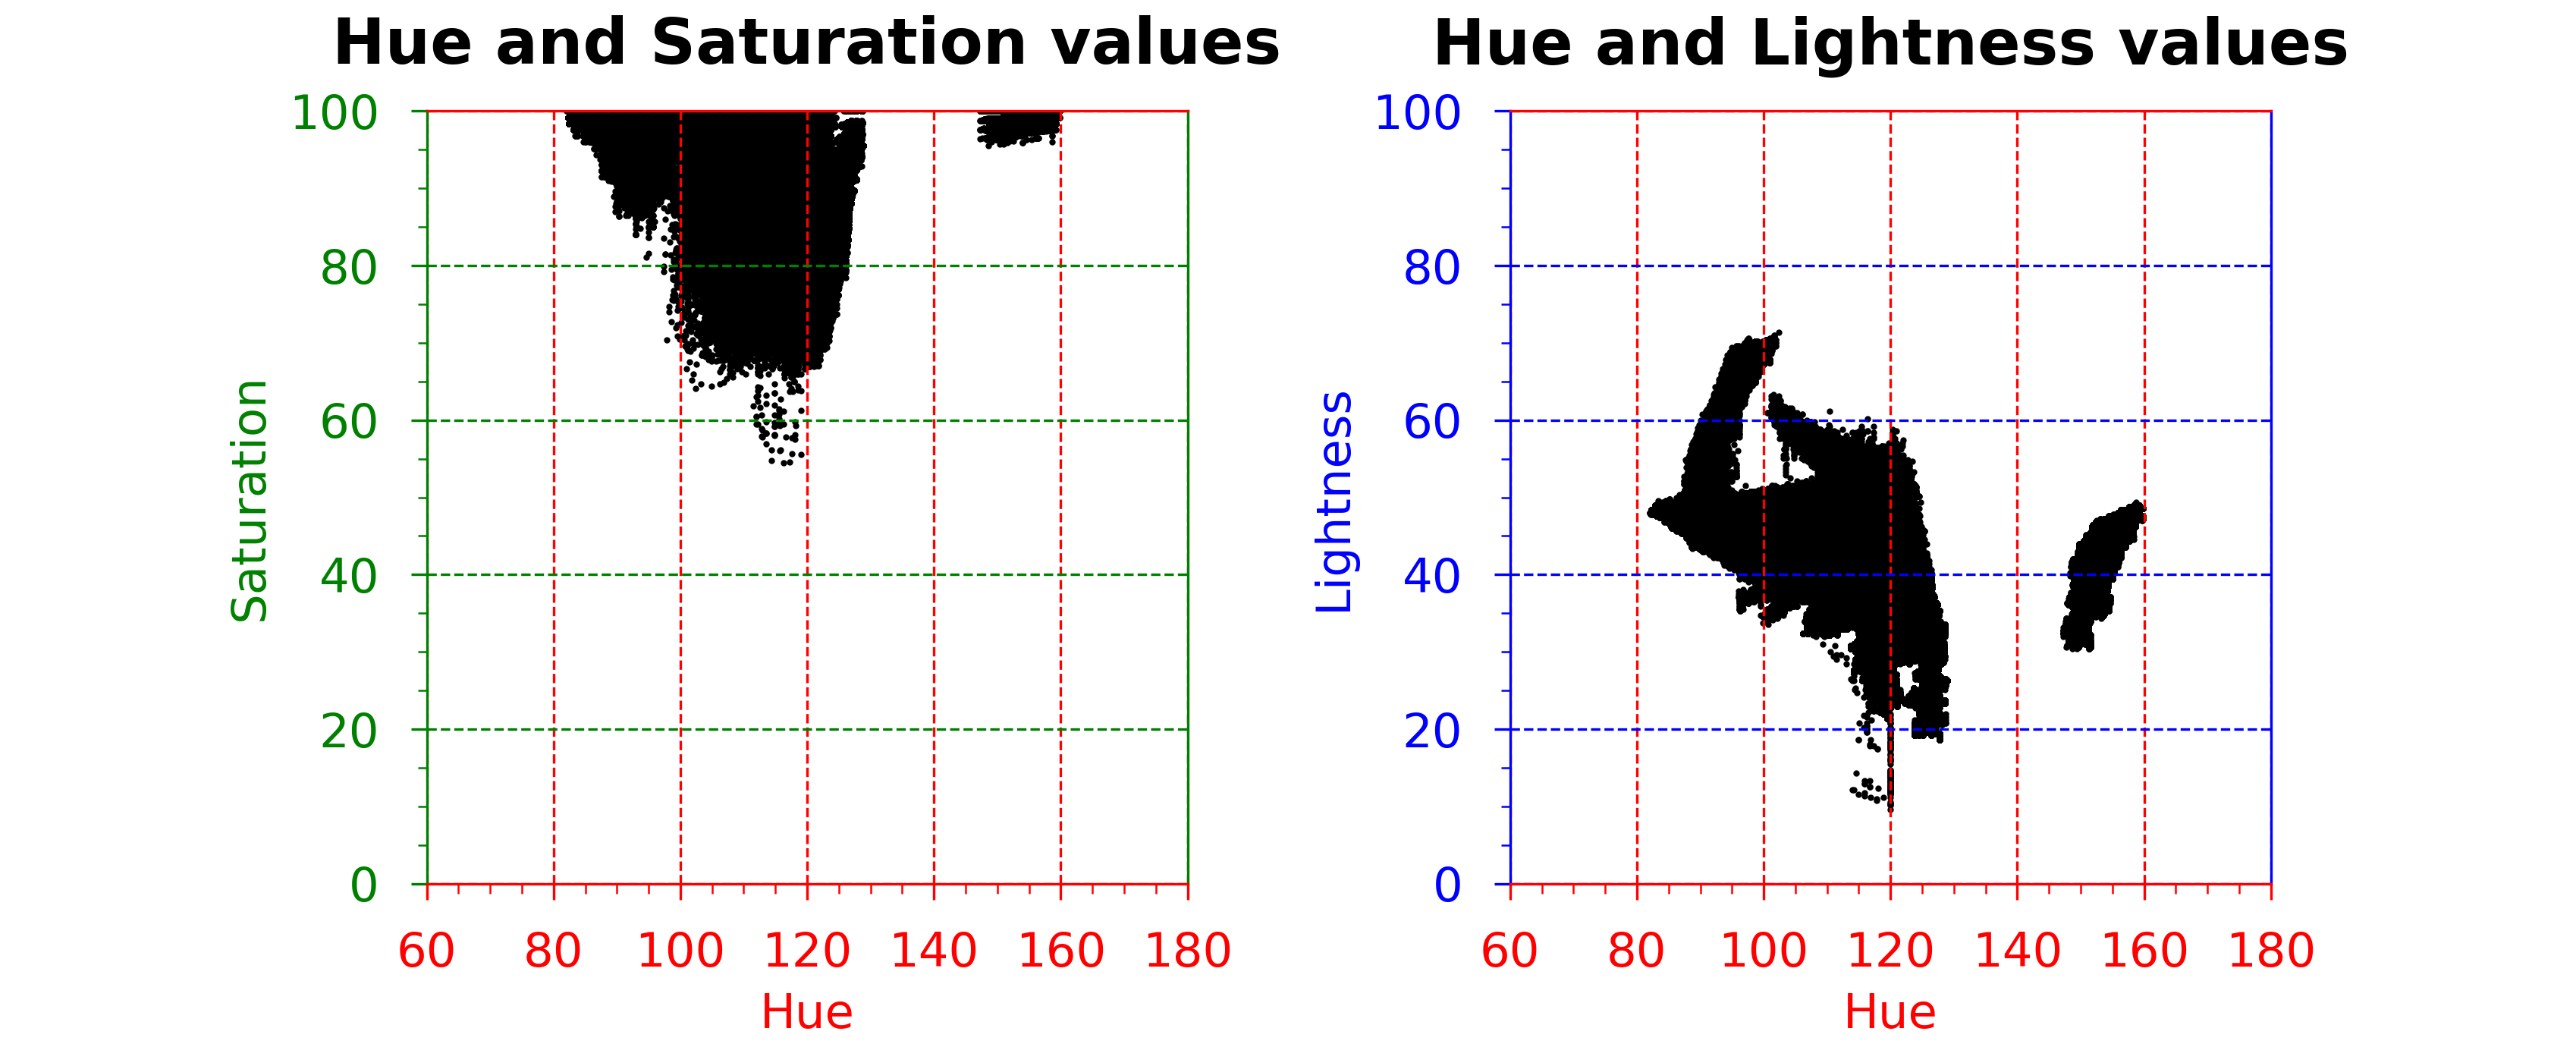
\includegraphics[width=\textwidth]{img/hslGreen.png}
	\caption{Scatter plots in functie van tint en saturatie, alsook in functie van tint en lichtheid voor de kleur groen.}
	\label{hslGreenPlot}
\end{figure}

\subsubsection{Verdere verbeteringen} \label{Verbeteringen kleur}
Uit de plots is echter gebleken dat aparte onderscheiding van zes verschillende kleuren geen goede optie is door overlap van de ranges van de verschillende kleuren. Dit is het gevolg van zeer verschillende waarnemingen van een kleur naargelang de omstandigheden waarin een foto getrokken wordt. Het is dus niet mogelijk om zes verschillende kleuren correct te onderscheiden in alle omstandigheden. Nieuwe methodes moeten gevonden worden waar niet zoveel verschillende kleuren van elkaar onderscheiden moeten worden. Een eerste mogelijkheid is om een detectie uitgaande van slechts drie kleuren te verkiezen boven een detectie met zes kleuren. Bij het gebruik van een drie-kleuren-detectie zijn twee opties, waarbij de kleuren opnieuw zo ver mogelijk van elkaar verwijderd liggen (120\degree),  mogelijk. Eenderzijds het gebruik van de kleuren rood, groen en blauw of anderzijds de kleuren cyaan, magenta en geel. De uiteindelijke keuze valt op rood, groen en blauw aangezien deze minder ver fluctueren van de theoretische waarde dan cyaan, magenta en geel. Aan deze optie wordt reeds gewerkt om de detectie te verbeteren. Daarnaast is het ook een optie om eerder relatief naar het contrast tussen kleuren te kijken in plaats van detectie op basis van absolute ranges. Ook deze optie wordt reeds bekeken om de identificatie te verbeteren.

\subsection{Flood fill}
Elk individueel slave scherm laat een vooraf bepaalde afbeelding zien met gekende kleur-waarden (*afbeelding van html). Deze afbeelding voor detectie is een combinatie van vorige iteraties van het project. Het combineren van een border met een kruis geeft het meeste informatie over de associatie van de kleur-gefilterde pixels bij overlap of afgedekte delen van het scherm en bovendien meer informatie over de oriëntatie van het scherm op de foto. Om deze schermen te detecteren wordt de foto gefilterd op basis van gekende HSL ranges (zie \ref{Ranges}) en een standaard four-way flood fill algoritme [4 way afbeelding of te veel?] \cite{floodfill} om de associatie van de verbonden pixels te behouden. Na de executie van de flood fill is er voor elk gedetecteerd eiland een pixel masker met een unieke ID per eiland, opgeslagen in elke pixel, waar de verdere bewerkingen op uitgevoerd zullen worden. Het geimplementeerde floodfill algoritme groeit volgens de vier pixel-buren en een stack-based iteratie process om recursie-overflow tegen te gaan bij grote afbeeldingen en eilanden. In een worst-case scenario zal dit algoritme een eiland detecteren over de volledige afbeelding. Aangezien elke pixel maximaal vier keer in de stack terecht kan komen, door zijn vier buren, loopt deze flood fill volgens een tijdscomplexiteit van 
\[O(4mn)=O(mn)\]
 met m en n de dimensies van de afbeelding. De grootte van elk eiland zal in de praktijk over het algemeen een stuk kleiner zijn dan de volledige afbeelding.

\begin{figure}[h]
\centering

\includegraphics[scale=0.5]{img/mask.png}
\caption{Kleurenmasker van een scherm na floodfill}
\end{figure}

Niet enkel de associatie van de gemaskeerde pixels wordt op deze manier behouden, maar deze methode maakt ook dat de komende bewerkingen maar over een minimale bounding box uitgevoerd worden ten opzichten van de volledige pixel matrix. Elk resulterend resultaat van floodfill geeft een verbonden pixel verzameling, een island, als resutlaat. De resulterende islands worden achteraf gefilterd opdat elk eiland de drie kleuren van de border en het middelpunt bevatten. Als er aan deze voorwaarde is voldaan is wordt er een poging gedaan om lokaal een middelpunt en geldige barcode te lezen \ref{barcode}. Bij het falen van een van deze verificatiestappen wordt het eiland verworpen, de overblijvende eilanden zijn geldige eilanden voor hoekdetectie.

\subsection{Hoekpunten}
Er werd vooraf een algemene hoek-detectie algoritme shi-tomashi geïmplementeerd en getest, maar gaf een te complex resultaat op de binaire maskers om de juiste hoeken te filteren. Dit algoritme draagt ook een relatief grote overhead door de x- en y-sobel operaties die elks een volledige pixel convolution over alle pixels in een eerste stap toepassen. Onze algoritmes zijn veel simplistischer en zullen in de praktijk nooit verder dan de boundary van een eiland uitgevoerd worden in tegenstelling tot de volledige island matrix, maar geven een perfect bruikbaar resultaat voor onze noden.

In de eerste stap wordt er bepaald of het scherm voornamelijk recht of gekanteld is ten opzichte van de foto. Hiervoor wordt langs de linker kant van het kader de standaarddeviatie van pixels in het masker berekend. Bij een standaardafwijking onder de 15\% wordt een scherm als liggend of verticaal gezien op de foto en niet gekanteld.\\
Als in eerste instantie het scherm als gedraaid beschouwd wordt, zal er vanuit elke rand van de bounding box van het eiland het de eerste mask-pixel als corner beschouwd worden. In het gev  al dat het scherm relatief horizontaal of verticaal recht staat, zal er loodrecht op de randen gezocht worden (zie figuur: \ref{fig:perp search}), maar volgens een diagonaal tot een mask-pixel (zie figuur: \ref{fig:diag search}).\\
\begin{figure}[h] 
\centering
\begin{subfigure}{0.5\textwidth}
\centering

\includegraphics[width=0.9\textwidth]{img/perpSearch.png}
\caption{Loodrechte corner search}
\label{fig:perp search}
\end{subfigure}%
\begin{subfigure}{0.5\textwidth}
\centering

\includegraphics[width=0.9\textwidth]{img/diagSearch.png}
\caption{Diagonale corner search}
\label{fig:diag search}
\end{subfigure}
\caption{Hoekdetectie}
\end{figure}

Beide variaties van hoek-detectie zal altijd vier hoeken als resultaat opleveren. Dit zullen door overlap en foutjes in het maskeren niet altijd correcte hoeken zijn. Na het bepalen, worden de hoeken nagekeken of deze resultaten wel degelijk kwalificeren als hoek. Deze kwalificatie is gebaseerd op bepaalde eigenschappen die in de buurt van elke hoek moeten gevonden worden, namelijk twee lijnen die tot de boord behoren en een diagonaallijn die naar het middelpunt van het scherm loopt \ref{fig:correcte hoek}. Deze lijnen zijn bepaald door te filteren door de border- en diagonaal-kleur die gescheiden zijn door een witte rand (*beter verwijzen naar waar calccircle wordt uitgelegd in reconstructie?). Als in een eerder gevonden hoek deze voorwaarden niet aanwezig zijn, wordt deze hoek verworpen \ref{fig:foute hoek}.

\begin{figure}[h] 
\centering
\begin{subfigure}{0.5\textwidth}
\centering
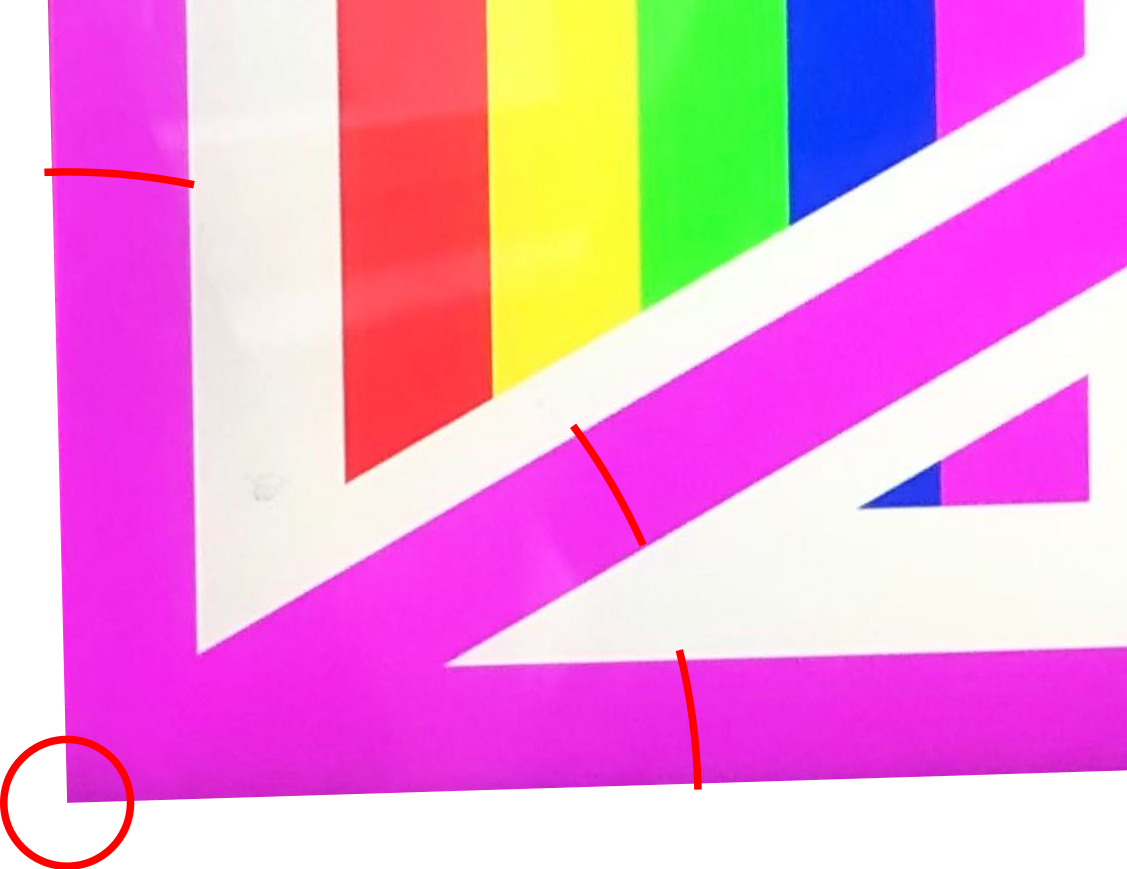
\includegraphics[width=0.6\textwidth]{img/correctCorner.png}
\caption{Een correcte hoek}
\label{fig:correcte hoek}
\end{subfigure}%
\begin{subfigure}{0.5\textwidth}
\centering
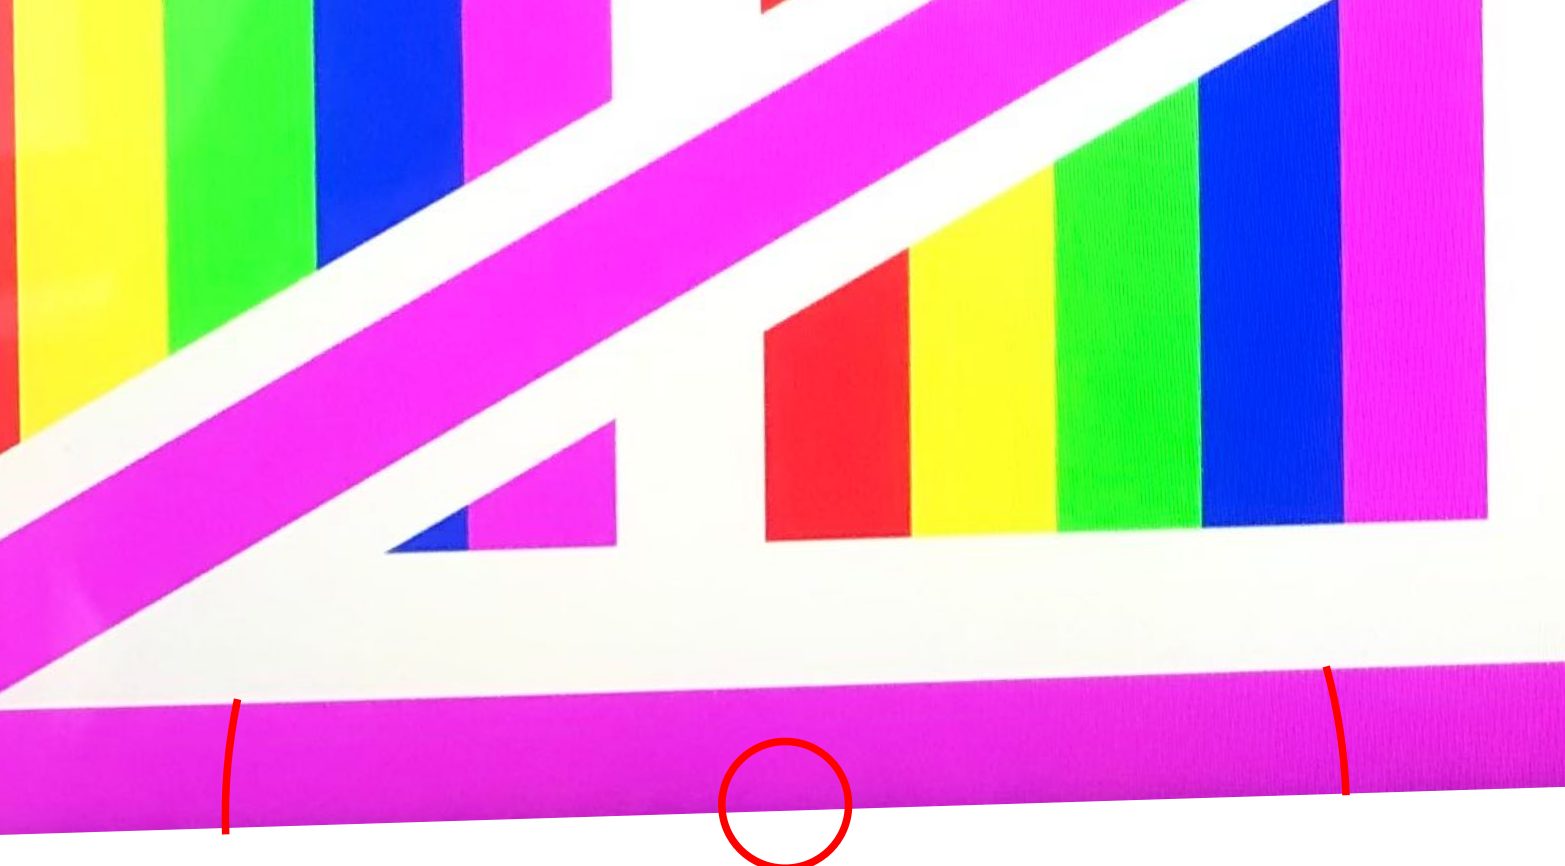
\includegraphics[width=0.6\textwidth]{img/notACorner.png}
\caption{Hoek zonder volledige features}
\label{fig:foute hoek}
\end{subfigure}
\caption{Hoekfiltering}
\end{figure}
(linken/binden naar reconstruction) Als er geen vier correcte hoeken gevonden worden, zullen missende hoeken gereconstrueerd worden uit de wel gevonden hoeken en het middelpunt.

\section{Reconstructie}\label{sec:reconstructie}

	Na het filteren van de hoeken kan het dus voorkomen dat er geen vier meer overblijven. Volgende kunnen hiervoor de oorzaak zijn. Enerzijds is het mogelijk dat bepaalde delen van schermen elkaar overlappen in de opstelling, anderzijds kunnen één of meerdere hoeken niet of slecht detecteerbaar zijn door een obstakel. Er wordt opgelegd dat minstens twee aanliggende hoekpunten en het middelpunt zichtbaar zijn. Indien men zich aan deze vooropgestelde eis houdt kan met volgend algoritme het scherm steeds volledig gereconstrueerd worden. Na een opsomming van de stappen volgt een meer gedetailleerde uitleg.
	\paragraph{Algoritme}
	 De input die wordt meegegeven is een dictionary van de reeds gevonden hoekpunten. De sleutels zijn LU,RU,RD en LD m.a.w. posities van hoeken en als bijhorende waarden coördinaten voor deze die reeds gevonden zijn en een \textit{null} als plaatshouder voor de nog te reconstrueren hoeken. \newline
	 Eerst worden de vier punten bepaald die zich rond het middelpunt op de diagonalen bevinden. Deze worden ook in een dictionary opgeslaan met dezelfde structuur als de input. Daarna wordt hoek per hoek gekeken welke nog ontbreken. Indien reconstructie nodig is, wordt het overeenkomende punt van de diagonalen genomen. Samen met het middelpunt wordt hieruit een eerste reconstructielijn opgesteld. Daarna wordt vanuit een aanliggend hoekpunt het laatste hulppunt bepaald waardoor de tweede rechte wordt getrokken. De gezochte hoek is dan het snijpunt van de twee constructielijnen. Deze stappen herhalen voor andere ontbrekende hoeken resulteert in een dictionary met alle hoekenpunten van het scherm. Hieronder volgt een uitgebreidere uitleg van gebruikte methodes met veronderstellingen, voordelen en nadelen.
	
	\subsection{Hulppunten op diagonalen} \label{subsec:diagonalen}
		
		Telkens wanneer reconstructie nodig is zulllen de punten op diagonalen rond het middelpunt bepaald en geordend opgeslaan worden in een dictionary. Hiervoor worden alle pixels overlopen die op de cirkel met een bepaalde radius rond het middelpunt liggen overlopen. De straal van deze cirkel wordt gedefiniëerd als een vierde van de grootste afstand tussen de reeds gevonden hoeken en het middelpunt. Op deze manier wordt rekening gehouden met de grootte van het scherm. 25 procent van deze afstand nemen zorgt ervoor dat de pixels niet tot het middelpunt behoren en er zich tegelijkertijd niet te ver van bevinden. 
		\paragraph{Startpunt} Het startpunt van waaruit de cirkel doorlopen wordt, is een pixel die niet tot een diagonaal behoord. Waarom dit belangrijk is zal later duidelijk worden. Bepalen of een punt deel uitmaakt van een diagonaal gebeurt aan de hand van een functie die controleerd of er zich tussen de desbetreffende pixel en een tweede meegegeven punt (in dit geval het middelpunt) een wit deel pixels bevindt. Indien er tussen de twee meegegeven punten een stuk wit voorkomt, betekend dit dat de pixel afkomstig is van een deel barcode \ref{Foto van screendetectie html!!!!} (*verwijzing foto van screendetectie html).
		Doordat de kleuren van de boord en diagonalen ook in de barcode voorkomen, sluit deze functie dus eigenlijk uit dat stukjes barcode toegevoegd worden aan de lijst. Het interval waarmee de hoek van nul tot twee keer pi loopt is één procent, hiermee worden net genoeg pixels overlopen. Naar later toe zou deze waarde ook relatief kunnen gezet worden naar de grootte van het scherm. Voor elke aaneenschakeling van pixels die geen wit kruisen op hun pad naar het middelpunt wordt een lijst aangemaakt tijdens het doorlopen van de cirkel. Uiteindelijk heeft men dan vier sublijsten van pixels in een lijst die elk een diagonaal voorstellen. Uit elke lijst wordt dan het middelste element genomen die het midden van dat cirkelsegment is. Hier komt al een eerste voordeel van het bepaalde startpunt naar voor. Indien dit niet gedaan zou worden kon het voorkomen dat een cirkel binnen een diagonaal startte. Dit zou resulteren in meer dan vier lijsten die aangemaakt worden wat het bepalen van de middens aanzienlijk complexer zou maken. 
		\paragraph{Ordenen} Zoals eerder vermeld worden deze vier punten dan vanuit een lijst geordend in een dictionary geplaatst. Als referentie wordt gestart vanuit de HTML voor de schermdetectie. Daarin zijn de twee bovenste hoeken geel en de onderste roze. Door de manier waarop de punten bepaald werden (het doorlopen van een cirkel) zitten de gele en roze pixels alreeds bij elkaar. Dus moet enkel nog gecontroleerd worden of de twee gele punten de eerste twee elementen in de rij zijn. Is dit niet het geval wordt de lijst geroteerd totdat aan de voorwaarde is voldaan. Elk element wordt dan in die volgorde toegevoegd aan de dictionary waardoor de punten telkens dezelfde ordening zullen hebben.
		
	\subsection{Reconstrueren van een hoekpunt}
		
		Indien een hoekpunt moet gereconstrueerd worden m.a.w. de waarde van de desbetreffende sleutel in de dictionary van hoekpunten is \textit{null}, wordt in de daarnet aangemaakte dictionary het bijhorende punt op de diagonaal geselecteerd. Als bijvoorbeeld de bijhorende waarde van LU \textit{null} is, wordt in de dictionary van punten op de diagonalen ook de waarde van LU geselecteerd.  Vanuit dit punt en het middelpunt kan de vergelijking voor een rechte opgesteld worden die de eerste constructielijn zal vormen. Een aanliggend hoekpunt met gekende coördinaat, hulphoek genaamd, zal door de voorwaarde van minstens twee aanliggende detecteerbare hoeken steeds gevonden worden. Vanuit deze worden weer de cirkelsegmenten van boorden en diagonaal bepaald, dit met de radius die berekend werd in \ref{subsec:diagonalen}. Met als grote verschil dat nu niet de middens moeten bepaald worden maar de twee uiterste punten. Dit zullen dan de pixels zijn die op de rand van het scherm liggen. Hiervoor wordt van elk cirkelsegment het eerste en laatste element opgeslaan. Dit is meteen ook het tweede pluspunt van het startpunt, het zorgt ervoor dat de eerste en laatste pixel van de lijsten altijd de buitenste punten van een boord of diagonaal zijn. Dit stelt het mogelijk de lijst waarover geïtereerd moet worden te reduceren tot 6 pixels (2 punten per segment, 2 boorden en 1 diagonaal). De twee pixels die het verst van elkaar gelegen zijn zoeken in deze lijst is veel efficïenter dan alle punten van de segmenten te moeten overlopen. Door de offset en andere opgestapelde afrondingen kan het mogelijk zijn dat  kan het zijn dat op de rechte vanuit elke van deze punten naar de hulphoek pixels gekruist worden die niet dezelfde id hebben als dat punt van waaruit de rechte werd opgesteld. Indien dat het geval is wordt de dichtsbijzijnde pixel genomen op dat cirkelsegment waarvoor dit wel mogelijk is. Afhankelijk van de onderlinge ligging tussen het te reconstrueren hoekpunt en de hulphoek moet beslist worden welke van de twee berekende punten verder nodig zal zijn voor de reconstructie. Dit kan als volgt achterhaald worden. Ter referentie wordt eerst de rechte tussen hulp- en overstaande hoek van de te reconstrueren hoek bepaald. Dan wordt voor de twee te reduceren punten de rechte opgesteld met de hulphoek. Degene die de grootste hoek vormt samen met de referentie rechte, bevat het te behouden punt en deze vormt dan ook de tweede constructielijn. De nieuwe hoek wordt dan bekomen door het snijpunt van de twee constructielijnen te bepalen \ref{intersectie} (*ref naar wikipedia intersectie class line). Om de id van de nieuw bepaalde hoek te bepalen, kan gekeken worden naar de tegenovergestelde hoek die reeds gekend zal zijn. Is die roze dan is de nieuwe hoek geel en vice versa. 

\section{Identificatie}\label{sec:identificatie}
 \subsection{Barcode} \label{barcode}
Om de verschillende schermen te identificeren wordt gebruik gemaakt van een kleuren barcode. De barcode bestaat uit een herhalend patroon van 5 unieke kleuren telkens gevolgd door een witte lijn. Door het gebruik van deze witte lijn weet het algoritme waar het patroon eindigt en de volgende sequentie terug opnieuw begint. Het detecteren van deze 5 kleuren gebeurt aan de hand van opgestelde HSL ranges, zie \ref{Ranges}. Voor de identificatie van de slaves wordt dus een unieke combinatie van deze 5 kleuren weergegeven, zie figuur \ref{scherm}. Deze vormt dan een unieke vijfcijferige code, die gelinkt kan worden aan de bijhorende slave. Dit zorgt ervoor dat we in theorie een totaal van $5!$ ($=120$) verschillende schermen op één moment kunnen detecteren. Herhaling van het patroon heeft als resultaat dat bij overlap het scherm nog steeds geïdentificeerd kan worden. Het algoritme zal twee keer over alle pixels itereren. Hierdoor heeft het algorimte een tijdscomplexiteit van
\[O(2mn)=O(mn)\]
met m en n de dimensies van het eiland waarin de barcode gelezen wordt. Het algoritme gaat een keer horizontaal en een keer verticaal over de pixels. Op deze manier kan de barcode in alle mogelijke orientaties van het scherm gelezen worden. Vervolgens worden de HSL waarden van deze pixels bekeken om de overeenkomstige kleur van elke pixel te achterhalen. Wanneer een HSL waarde binnen de gewenste range valt, wordt het overeenkomstig cijfer opgeslaan in een lijst. Bij het bereiken van een witte lijn weet het algoritme dat het aan het einde van het patroon is. Wanneer dit het geval is, wordt het inlezen van de volledige vijfcijferige code gecontroleerd op volledigheid. Zo niet, wordt de lijst leeg gehaald en zoekt het algoritme verder. Het herhalend patroon is dus essentieel aan het correct inlezen van de barcode. Een groter aantal herhalingen stemt overeen met een hogere kans op mogelijke detectie, maar stemt ook overeen met een kleinere oppervlakte per herhaling. Deze kleinere oppervlakte is dan weer nadelig voor detectie. Aangezien hiermee de kans stijgt dat een kleur niet gededecteerd wordt. Nadat het algoritme over alle pixels geweest is, wordt de ratio berekend tussen de code die het meeste keer gelezen is en de totale aantal codes die zijn gelezen. Deze ratio bepaalt dan of de code, die door de horizontale iteratie of door de verticale iteratie het meest gelezen is, gebruikt wordt.

\begin{figure}[h!]
	\center
	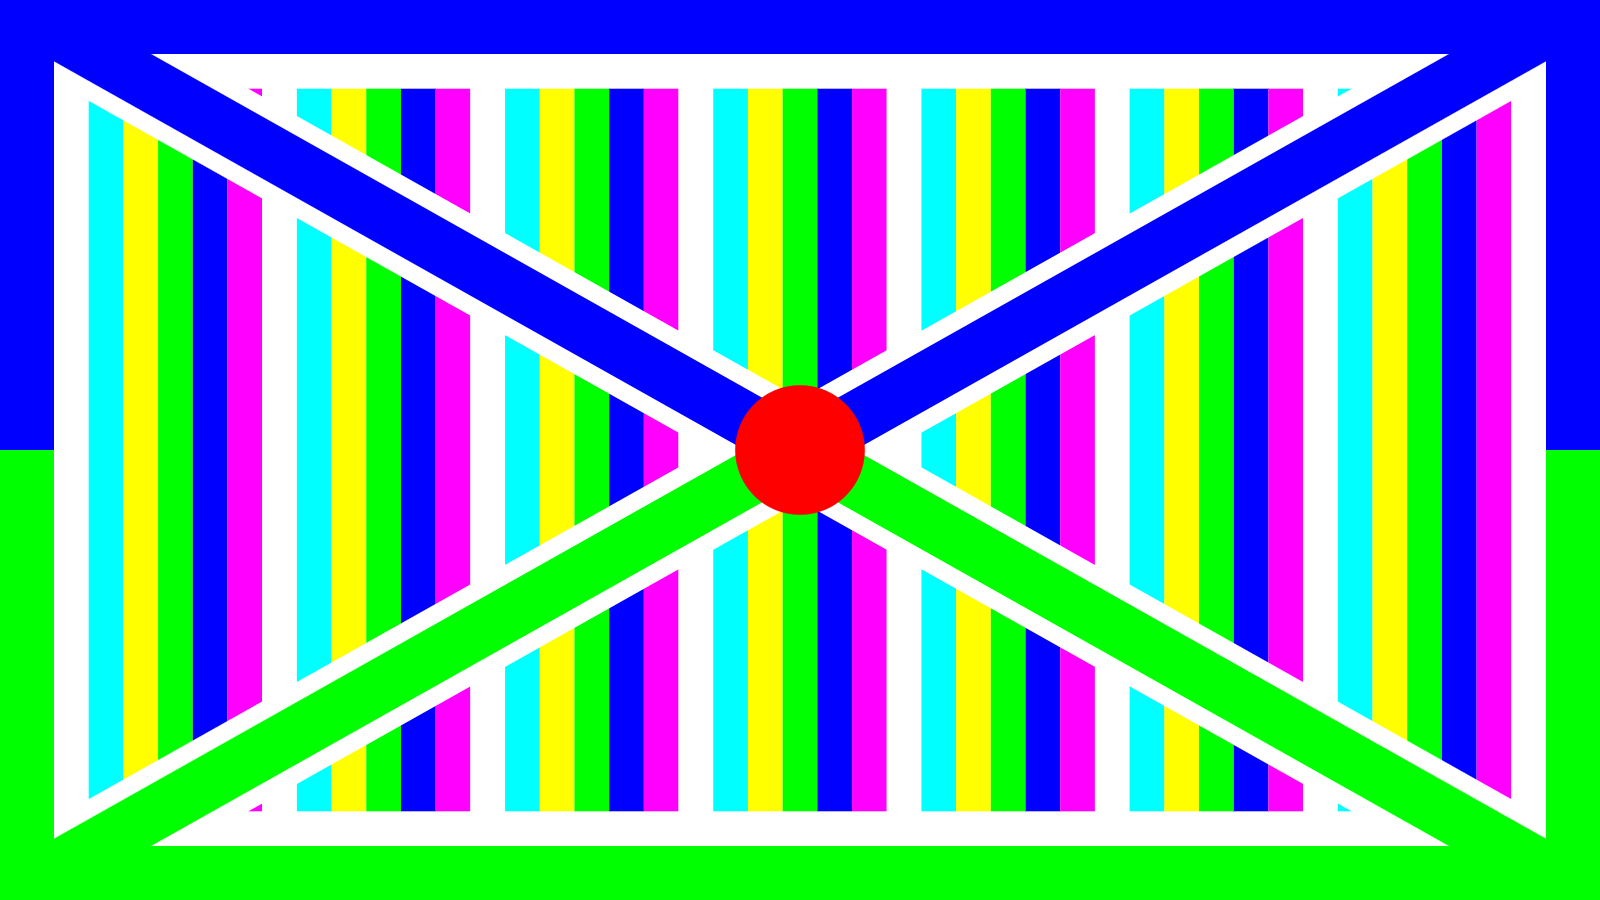
\includegraphics[width=0.8\textwidth]{img/screen.png}
	\caption{Scherm met randen en kruis voor detectie met barocde erachter voor identificatie.}
	\label{scherm}
\end{figure}

\subsection{Verdere verbeteringen}
Zoals reeds vermeld in \ref{Verbeteringen kleur} is het individueel dedecteren van zoveel verschillende kleuren geen goed idee. Dit is dan ook de reden dat andere opties reeds bekeken worden. Zoals ook reeds vermeld zou een eerste optie zijn om te kijken naar het contrast tussen de opeenvolgende kleuren in plaats van de kleuren apart te dedecteren. Een andere optie die bekeken wordt is het overschakelen naar een zwart-wit barcode waarbij gebruik gemaakt wordt van het contrast tussen zwart en wit. Een andere mogelijke verbetering is het aantal herhalingen afhankelijk maken van de grootte van het scherm. Dit heeft als voordeel dat het aantal herhalingen geoptimaliseerd is voor de grootte van het scherm.


\input{Transformatie voor image-show}

\section{Triangulatie} \label{sec:triangulatie}
Wanneer de schermen herkent en geïdentificeerd zijn, worden ze aan elkaar gelinkt door middel van een triangulatie. Het project gebruikt een Delaunay triangulatie. Dit is een speciale vorm waarbij de kleinste hoek gemaximaliseert wordt en waarbij de driehoeken niet overlappen \cite{delaunaywiki}.
Er wordt gebruik gemaakt van het Bowyer-Watson algoritme. \cite{Bowyer-WatsonWiki} Het heeft een tijdscomplexiteit van $O(n^2)$, dit is zeker niet de beste complexiteit om een Delaunay triangulatie te berekenen. Aangezien in de toepassing maximaal 120 schermen gebruikt kunnen worden, voldoet $O(n^2)$. Met de eenvoudige implementatie is dit dan ook een voordehandliggende keuze.

\subsection{Bowyer-Watson}
Bowyer-Watson gaat er van uit dat punten enkel worden toegevoegd in een al bestaande Delaunay triangulatie. Als eerste worden er twee superdriehoeken gezocht. Deze driehoeken zullen alle te trianguleren punten bevatten. De implementaties waarop het algoritme is gebaseerd \cite{Bowyer-WatsonWiki} \cite{bowyer-watsonImplementation} stelden beiden een `superdriehoek' voor, zie figuur \ref{bowyer-watson-a} Echter is het eenvoudiger om een omkaderende vierhoek te vormen en deze op te delen in twee driehoeken. Vervolgens worden alle punten één voor één toegevoegd.
\bigskip
Voor elk punt worden alle driehoeken gezocht waarvan het punt in de omschreven cirkel zit. Wanneer twee driehoeken eenzelfde zijde delen, wordt deze verwijderd. Alle punten van de omschreven veelhoek van de twee driehoeken worden nu verbonden met het toegevoegde punt, zie figuur \ref{bowyer-watson-b}. Met deze werkwijze zal er op elk moment een Delaunay triangulatie zijn en moeten de driehoeken achteraf niet meer overlopen worden. Met het gevolg dat het data management voor deze methode minder complex is.
\bigskip
Eens alle punten toegevoegd zijn, worden de driehoeken die één of meer hoeken van de omkaderende vierhoek bevatten verwijderd, zie figuur \ref{bowyer-watson-c}. Aangezien deze driehoeken aan de buitenkant liggen is dit toegestaan. Er zal een Delaunay triangulatie overblijven van alle onderzochte punten.

\begin{figure}[H]
	\center
	\begin{subfigure}{0.4\textwidth}
		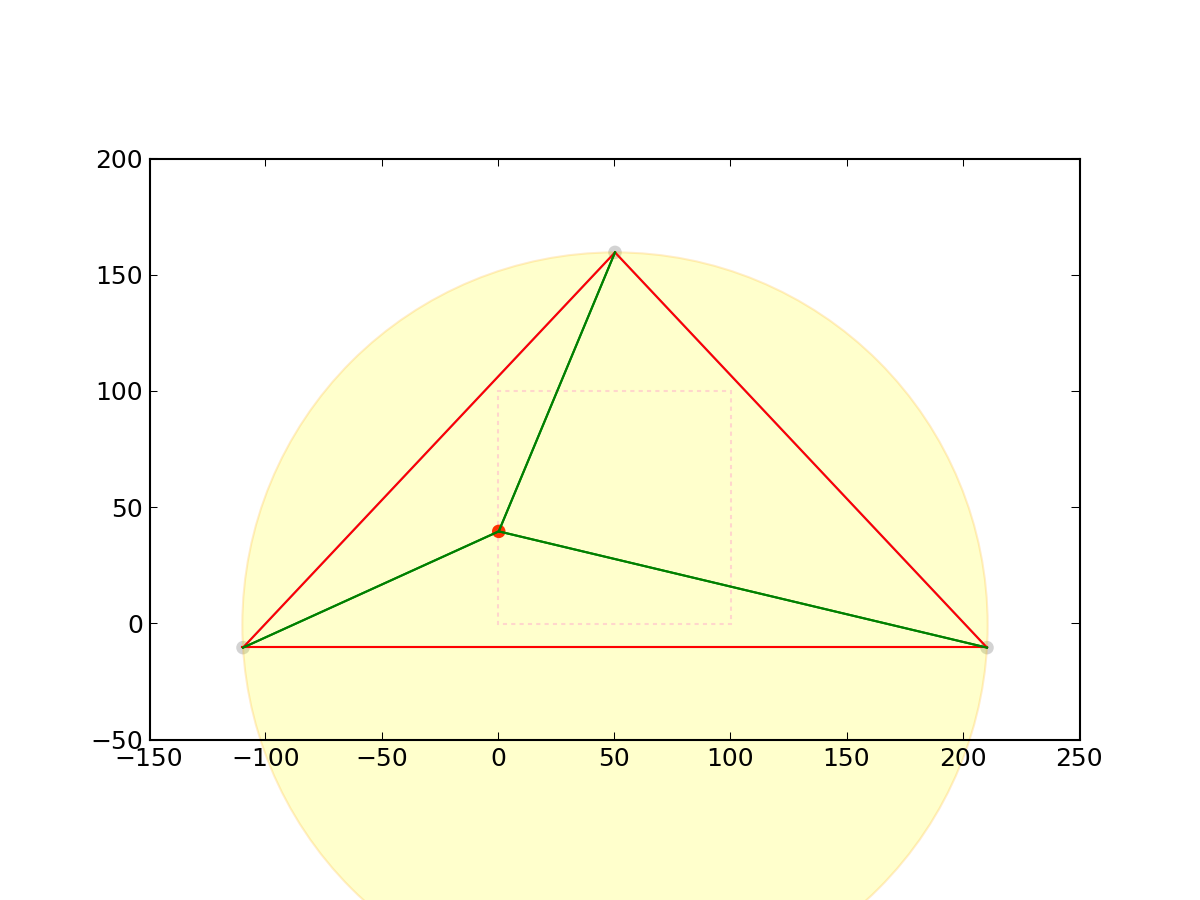
\includegraphics[width=\textwidth]{img/bowyer-watson_superdriehoek}
		\caption{De rode superdriehoek waarin alle punten zullen worden toegevoegd.}
		\label{bowyer-watson-a}
	\end{subfigure}
	\begin{subfigure}{0.4\textwidth}
		\includegraphics[width=\textwidth]{img/bowyer-watson_nieuwpunt}
		\caption{Een nieuw punt wordt toegevoegd. In geel de omschreven cirkels. De gestippelde zijde wordt verwijderd, de groene toegevoegd.}
		\label{bowyer-watson-b}
	\end{subfigure}
		\begin{subfigure}{0.4\textwidth}
		\includegraphics[width=\textwidth]{img/bowyer-watson_verwijderen}
		\caption{In rood alle driehoeken verbonden met de superdriehoek, deze worden uiteindelijk verwijderd.}
		\label{bowyer-watson-c}
	\end{subfigure}
	\caption{Het Bowyer-Watson algoritme \cite{Bowyer-WatsonWiki}}
	\label{bowyer-watson}
\end{figure}

\subsection{Valkuilen}
In theorie kan er van elke opstelling waarbij de punten niet allemaal colineair zijn een triangulatie worden gevonden, zie figuur \ref{colineair}. Echter door afronding bij de berekeningen zal er bij bijna colineaire punten geen juiste  configuratie gevonden worden, zie figuur \ref{almost_colineair}. 

\begin{figure}[H]
	\center
	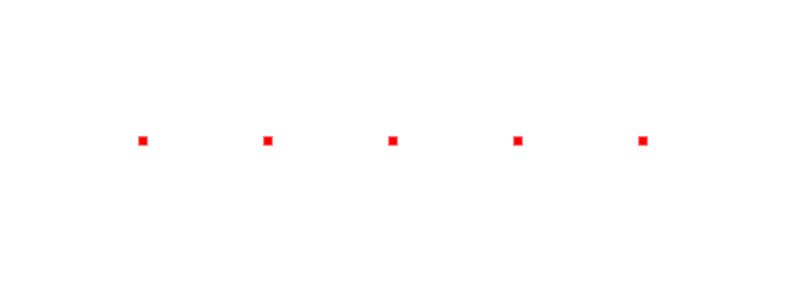
\includegraphics[width=0.4\textwidth]{img/colineair}
	\caption{Van colineaire punten kan geen triangulatie gevonden worden.}
	\label{colineair}
\end{figure}
\begin{figure}[H]
	\center
	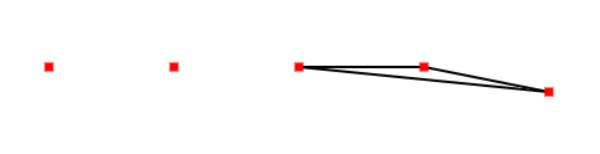
\includegraphics[width=0.4\textwidth]{img/almost_colinair}
	\caption{Van bijna colineaire punten kan geen triangulatie gevonden worden door afrondingsfouten bij berekeningen.}
	\label{almost_colineair}
\end{figure}



\section{Animation}


\subsection{Sprites}

De animatie van de kat of muis wordt bekomen door het snel achter elkaar tekenen van delen van een sprite sheet. Deze sheet bevat in dit geval 7 frames, zie figuur \ref{fig:cat} en \ref{fig:mouse}. De breedte van de sheet zal door het aantal frames worden gedeeld om zo met een "draw" methode elke deel appart en achter elkaar te displayen. Op deze manier creërt men de illusie van beweging op een zeer simpele manier. In dit geval loopt de kat of muis naar rechts maar met een spiegel methode kan de andere richting bekomen worden. De sprite zal ook worden geroteerd om in de correcte richting te bewegen. Meerdere muizen zullen achter elkaar loppen zodat op verschillende schermen sprites worden afgebeeld, zie figuur \ref{fig:schermen}. Dit werkt aan de hand van een stack waarin zich de vorige posities van de eerste kat bevinden. Na de laatste "draw" methode zal het eerste element van de lijst worden verwijderd. Alle dieren zullen dus hetzelfde pad nemen.

\begin{figure}[H]
\centering

\includegraphics[scale=0.2]{img/cat2.png}
\caption{Kat sprite sheet \cite{catsprite}}
\label{fig:cat}
\end{figure}

\begin{figure}[H]
\centering

\includegraphics[scale=0.8]{img/mouse2_trans.png}
\caption{Muis sprite sheet \cite{mousesprite}}
\label{fig:mouse}
\end{figure}


\newpage
\subsection{Delaunay}

Voor de animatie wordt gebruik gemaakt van de reeds geschreven delaunay triangulatie. Deze zal het pad vormen waarover de kat of muis zal lopen. Wanneer het dier zich dicht genoeg bij het endPoint bevindt zal deze de firstPoint worden en zullen de buren ervan opgevraagd worden. Er zal willeukeurig een punt worden gekozen als nieuw endPoint. Dit punt kan niet het firstPoint van de vorige beweging zijn. Dit wil zeggen dat de animatie nooit terug op zijn stappen komt. Enkel als de triangulatie een rechte lijn vormt zal de sprite op en neer lopen. 

\subsection{Server/Client side}

De server zal simpelweg de basis info doorgeven aan de client, zelf de berekeningen maken voor de volgende posities en de triangulatie bijhouden. De client krijgt enkel een dictionnary met de x,y positie, de hoek, de frame en een boolean voor spiegeling mee en heeft geen weet van de triangulatie.

\begin{figure}[H]
\centering
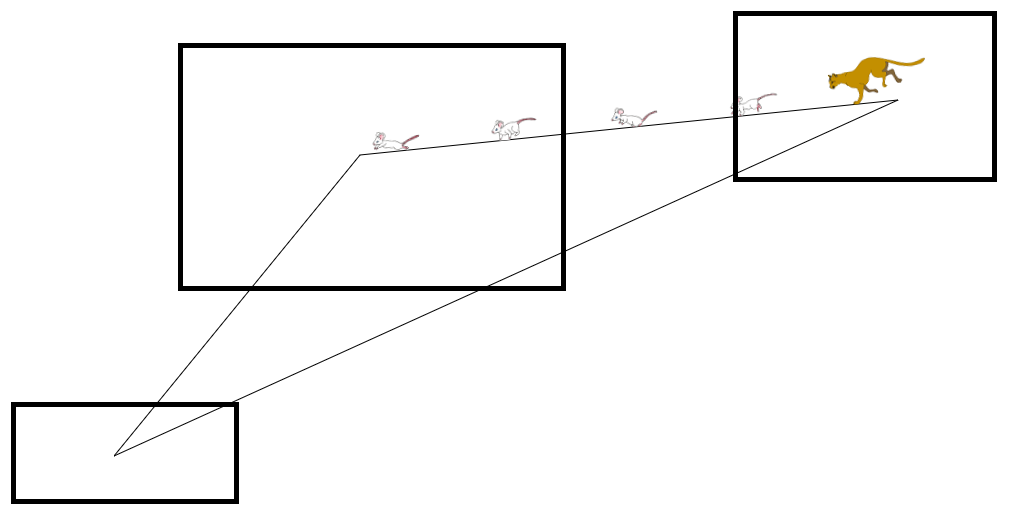
\includegraphics[scale=0.5]{img/schermen.png}
\caption{Theoretische animatie met verschillende schermen}
\label{fig:schermen}
\end{figure}



\section{Besluit}
Er is een applicatie ontwikkeld waarin een master verschillende cliënt schermen kan detecteren en manipuleren. Het framework houdt rekening met uitbereiding naar verschillende {\it kamers}. Voor video wordt er gestreamd in plaats van volledig gedownload. Met behulp van synchronisatie zal een video of een aftelklok gelijk lopen op elk scherm. Enkel bij uitzonderlijke gevallen waarbij de {\it ping} toevallig fout wordt gemeten (door bv. actieve achtergrondprocessen) kan er een synchronisatiefout optreden.
\bigskip
Het master device kan vanuit één enkele foto alle schermen herkennen. Hierbij wordt gebruik gemaakt van een bepaald herkenningspatroon. Bij sterke reflectie, grote 3d-draaiing en verschillende kleurweergave van de schermen kan het mislopen. Schermen worden dan niet herkent en zullen dus niet kunnen samenwerken met de herkende schermen. Een oplossing wordt hiervoor gezocht in de vorm van kleurverschil i.p.v. kleurdetectie. Hiervoor zijn er al plots opgesteld om de reikwijdte van de verschillende kleuren te determineren en zo de kleurschema's beter en efficiënter te gebruiken.
\bigskip
Het reconstrueren van schermen, wanneer er een deel van het scherm wordt bedekt, vertrouwd er op dat er 2 aanliggende hoeken en het middelpunt wordt gevonden. Met behulp van een transformatiematrix wordt de ligging en draaiing van het scherm bepaald. Hierdoor kan een afbeelding met juiste transformaite geprojecteerd worden op elk scherm. Deze heeft echter vier hoeken nodig en bouwt verder op de reconstructie van het scherm.
\bigskip
Als laatste is er nog de animatie die zeer nauw samenhangt met de triangulatie. Hiervoor is een Delaunay triangulatie gekozen omdat deze uniek is, niet overlappend en voor een maximale kleinste hoek streeft. Wanneer alle punten (bijna) colineair zijn, zal er door afronding geen triangulatie gevonden worden, de animatie kan dan ook niet worden afgespeeld.
\bigskip
De applicatie heeft een brede waaier aan functionaliteiten. Doordat er maar één foto nodig is voor de schermen te herkennen, is het plaatsen van de schermen nauwkeurig maar kan de identificatie sneller mislopen. Alle opdrachten, exclusief de cat caster, zijn geïmplementeerd. Met enkel nog een paar kleine {\it bugs}, waarnaar gestreefd wordt deze op te lossen, is er spraken van een geslaagde opdracht.

\newpage
\bibliographystyle{unsrt}
\bibliography{Bibliography}

\newpage
\appendix
\section{Kleuren plots}\label{sec:Kleuren plots}

\subsection{RGB plots}

\begin{figure}[h!]
	\centering
	\begin{minipage}{0.5\textwidth}
		\centering
		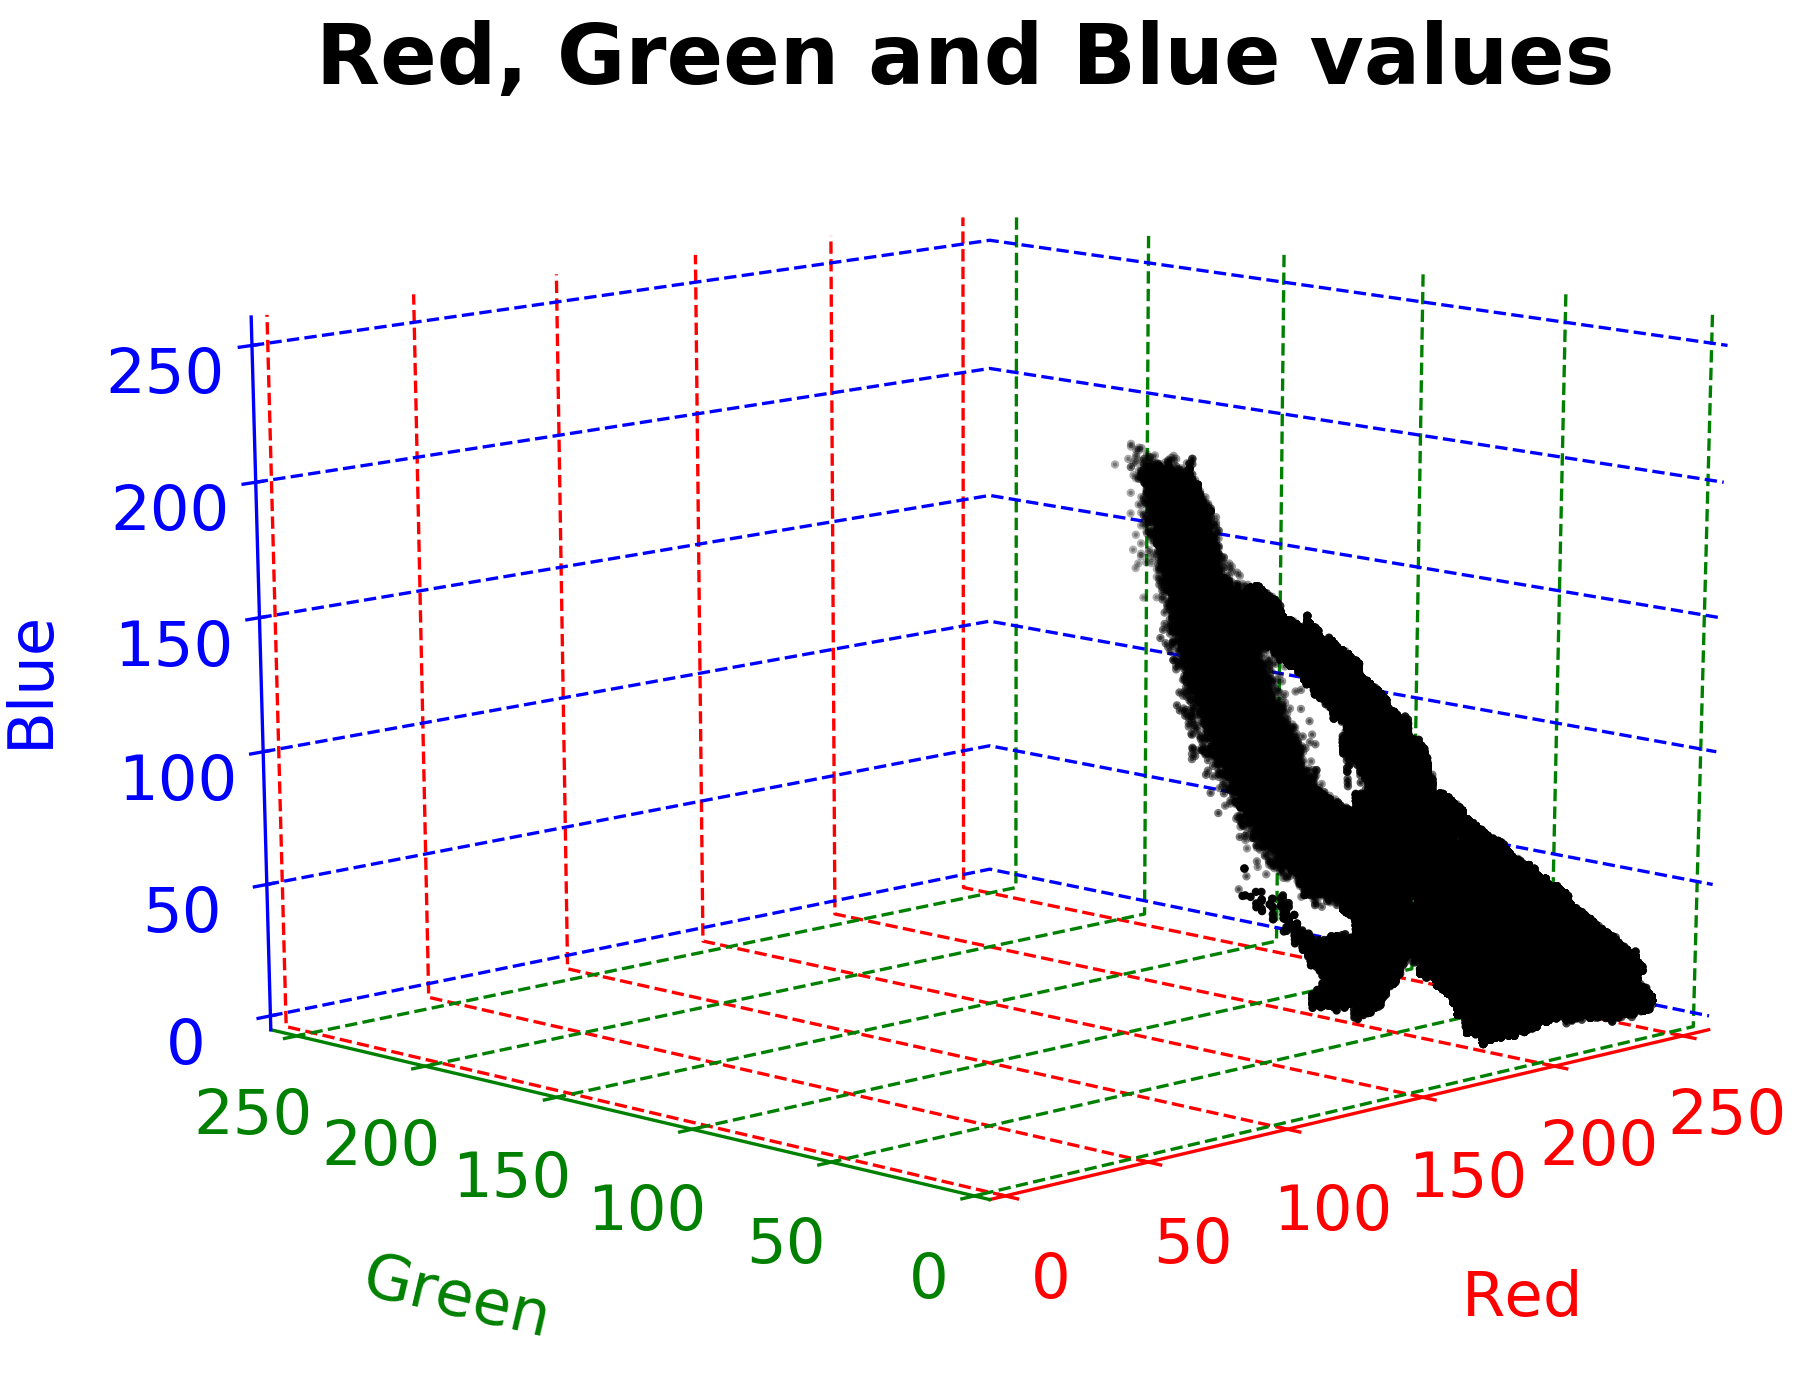
\includegraphics[width=0.9\textwidth]{img/rgbRed.png}
		\captionsetup{width=0.9\textwidth}
		\captionof{figure}{RGB plot voor de kleur rood.}
		\label{rgbRedPlot}
	\end{minipage}%
	\begin{minipage}{0.5\textwidth}
		\centering
		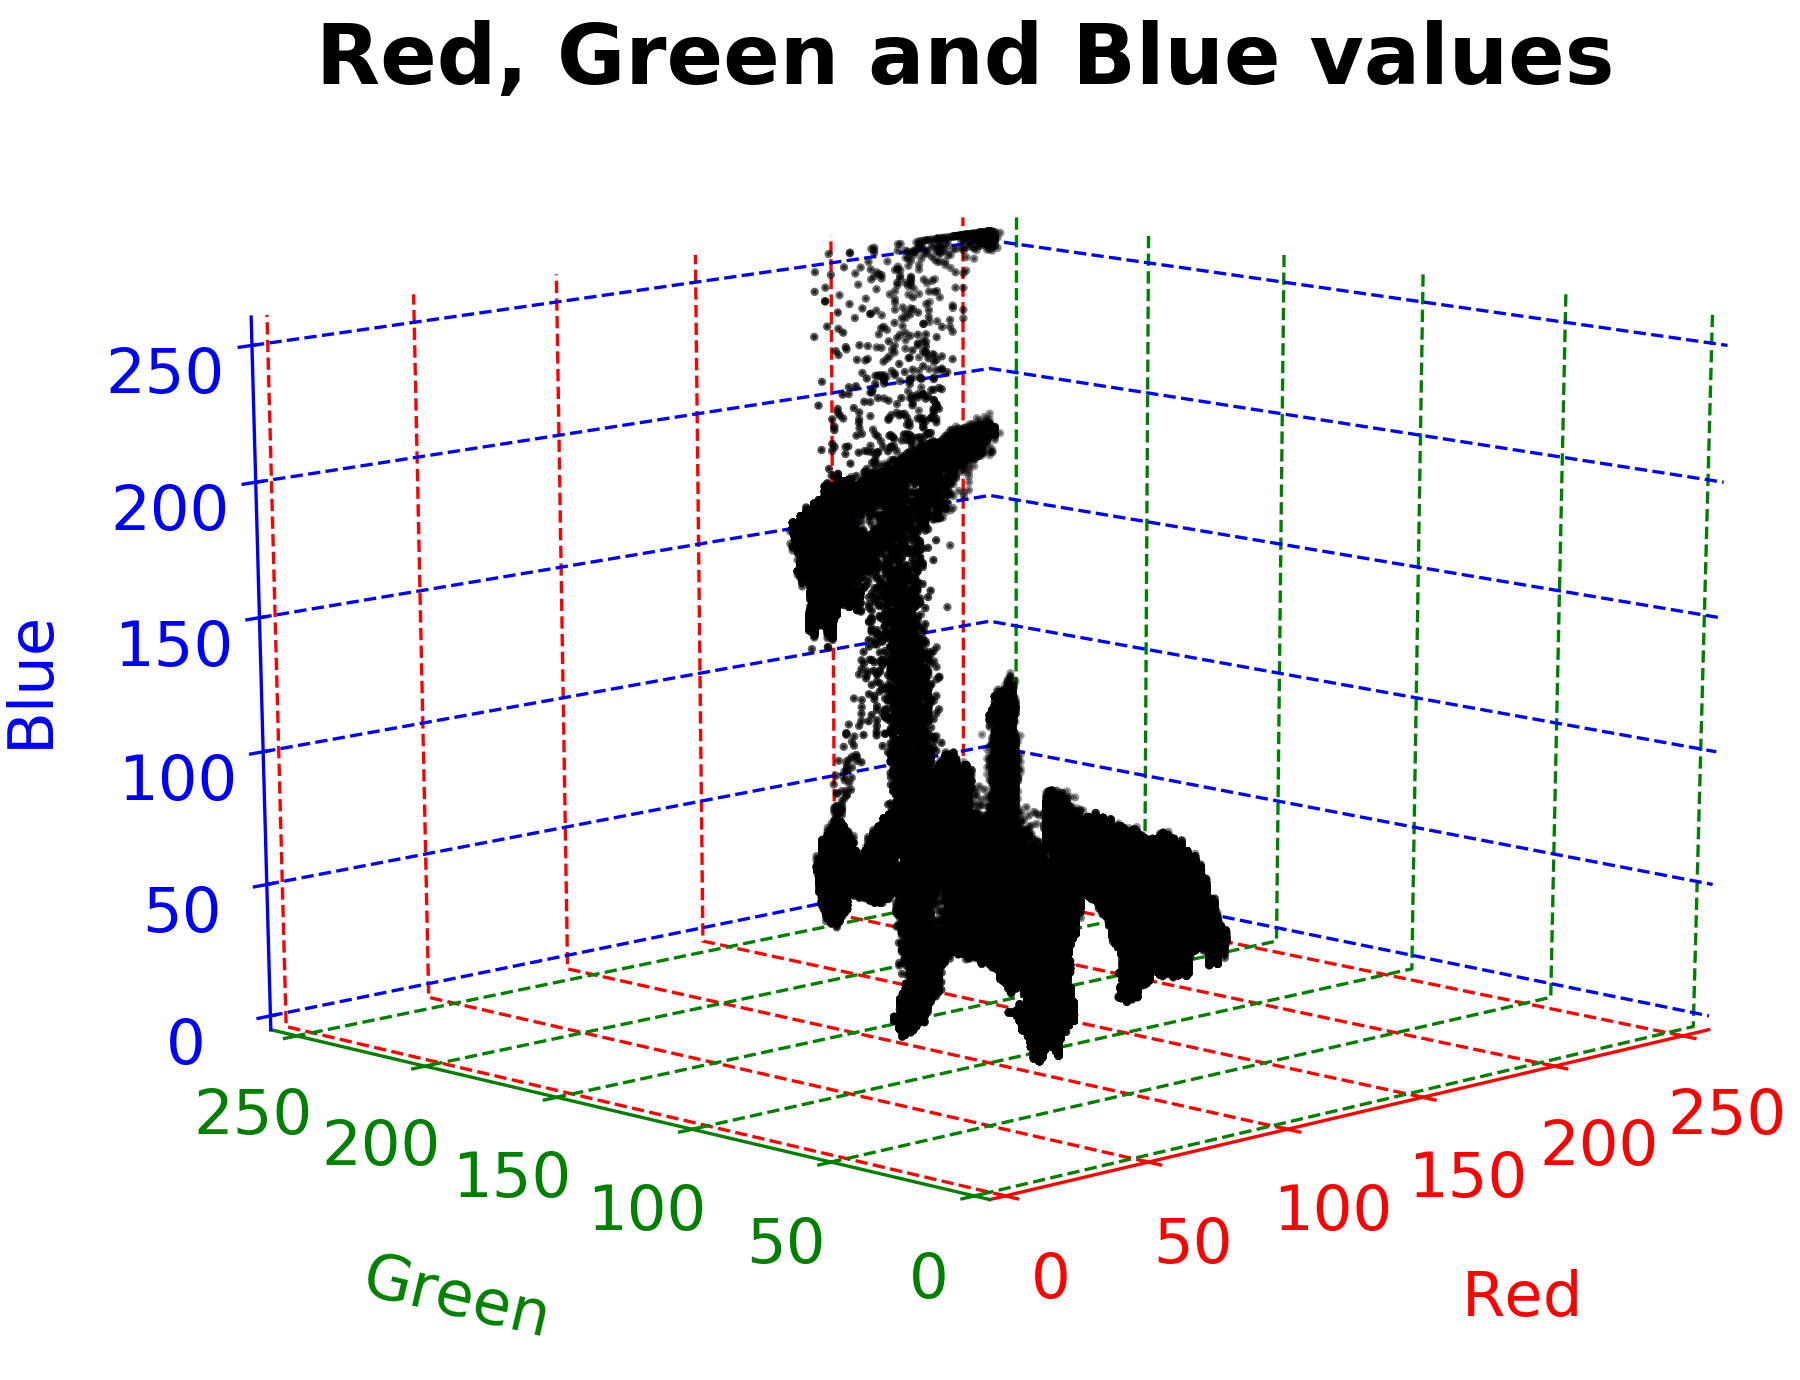
\includegraphics[width=0.9\textwidth]{img/rgbYellow.png}
		\captionsetup{width=0.9\textwidth}
		\captionof{figure}{RGB plot voor de kleur geel.}
		\label{rgbYellowPlot}
	\end{minipage}
\end{figure}

\vspace{5mm}

\begin{figure}[h!]
	\centering
	\begin{minipage}{0.5\textwidth}
		\centering
		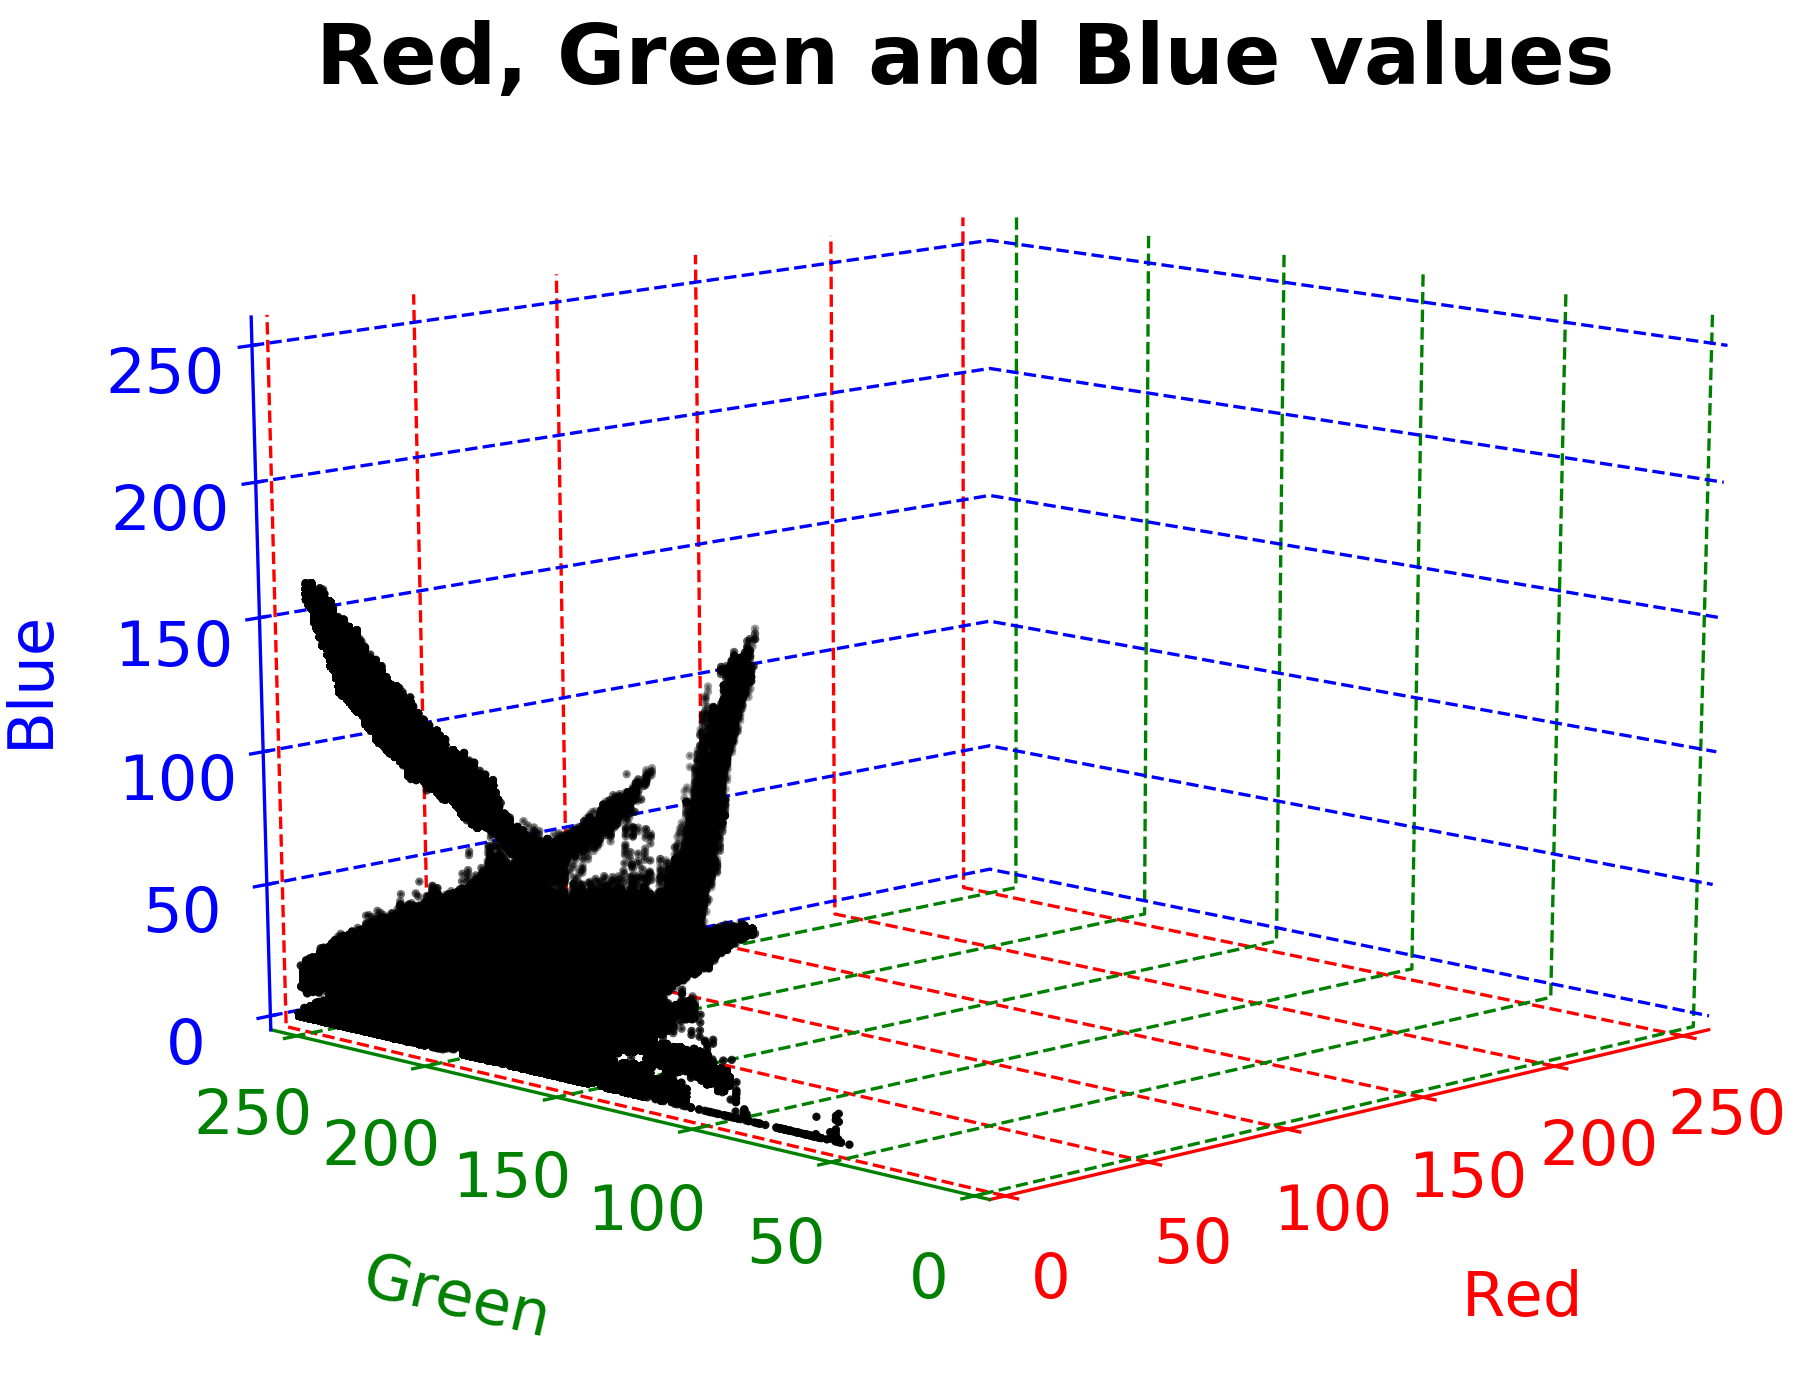
\includegraphics[width=0.9\textwidth]{img/rgbGreen.png}
		\captionsetup{width=0.9\textwidth}
		\captionof{figure}{RGB plot voor de kleur groen.}
		\label{rgbGreenPlot}
	\end{minipage}%
	\begin{minipage}{0.5\textwidth}
		\centering
		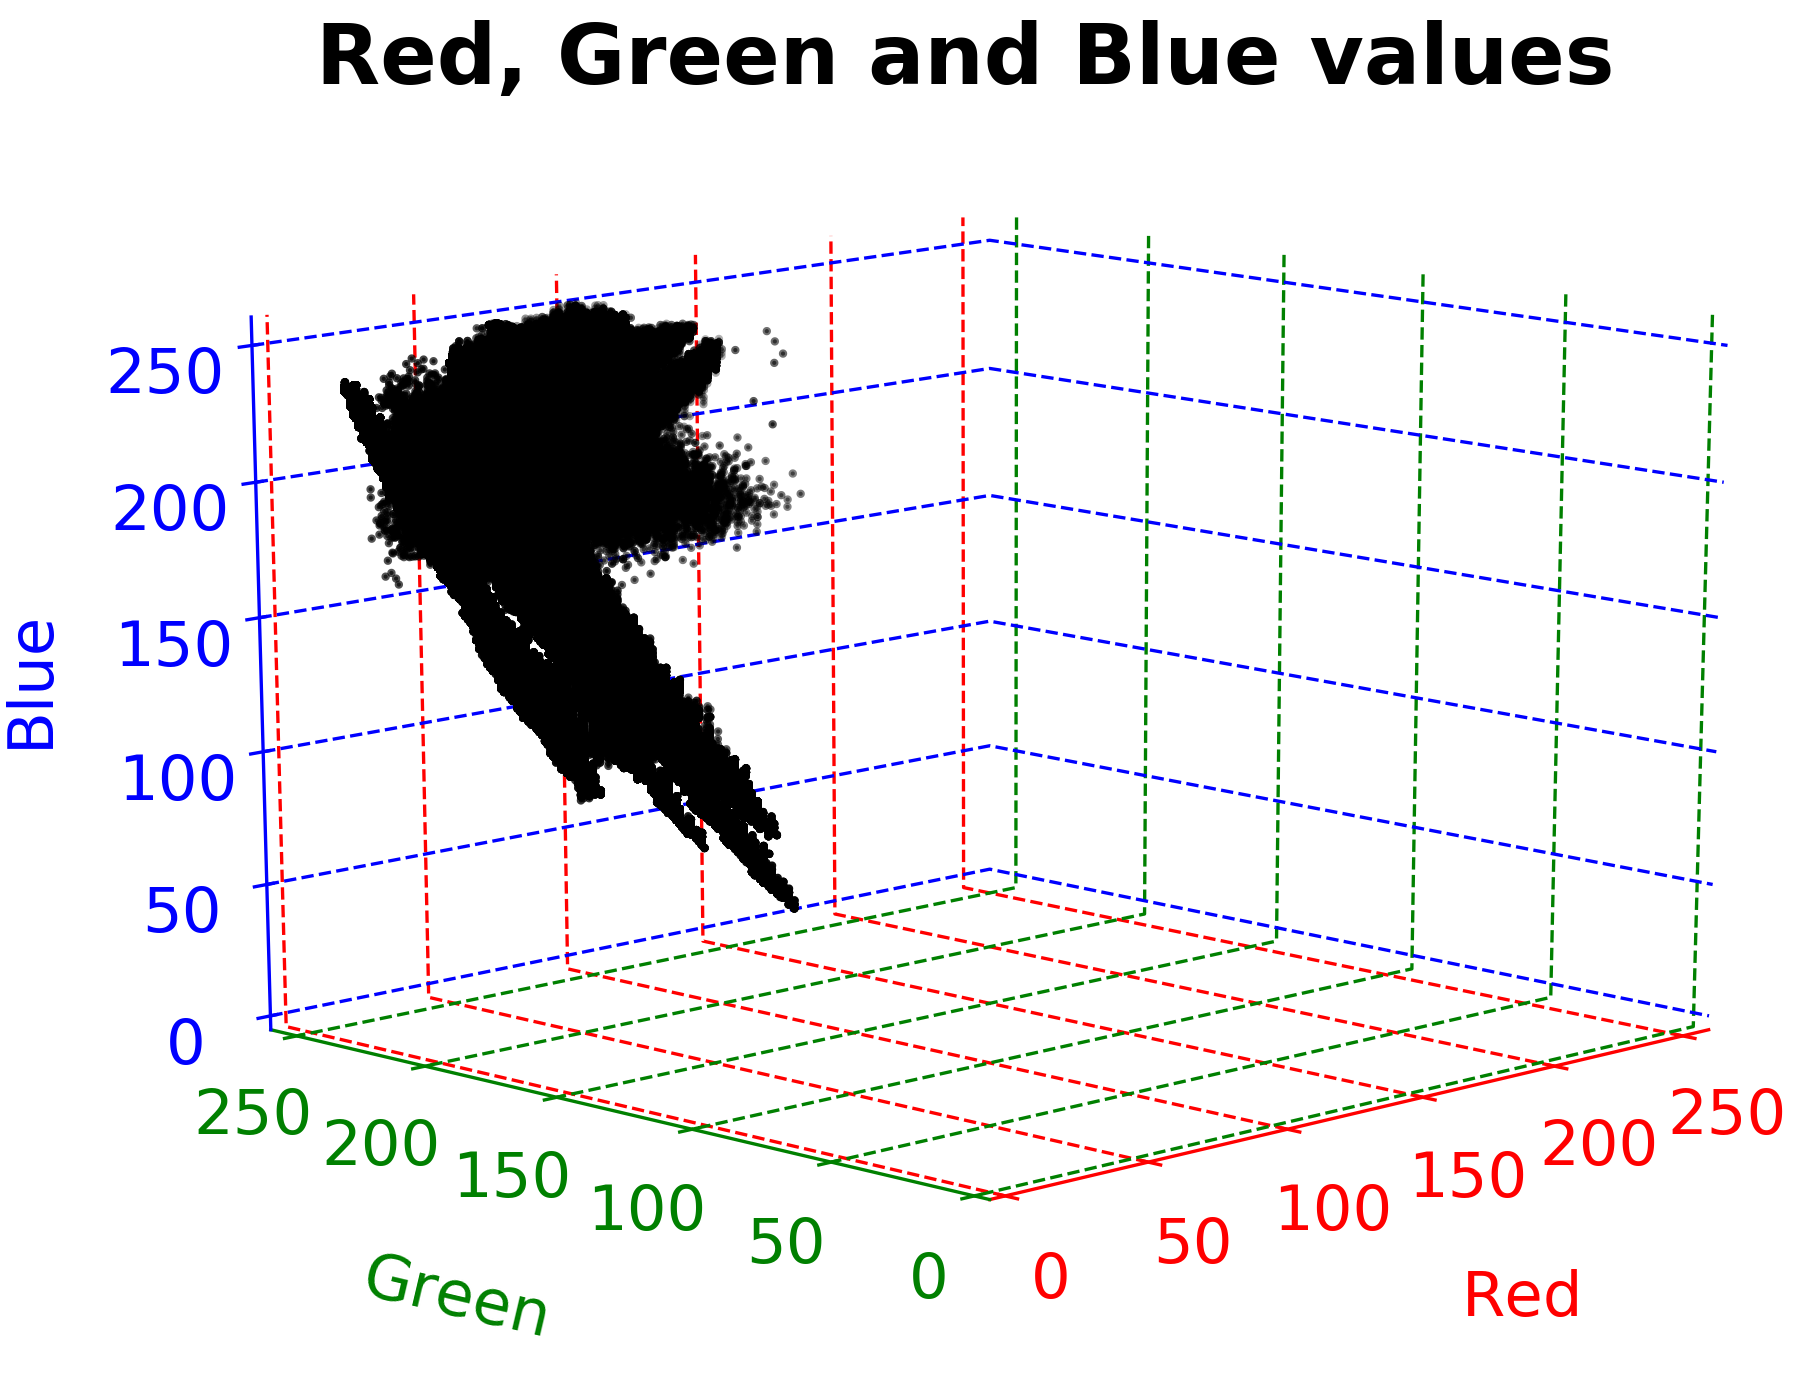
\includegraphics[width=0.9\textwidth]{img/rgbBlueGreen.png}
		\captionsetup{width=0.9\textwidth}
		\captionof{figure}{RGB plot voor de kleur cyaan.}
		\label{rgbBlueGreenPlot}
	\end{minipage}
\end{figure}

\vspace{5mm}

\begin{figure}[h!]
	\centering
	\begin{minipage}{0.5\textwidth}
		\centering
		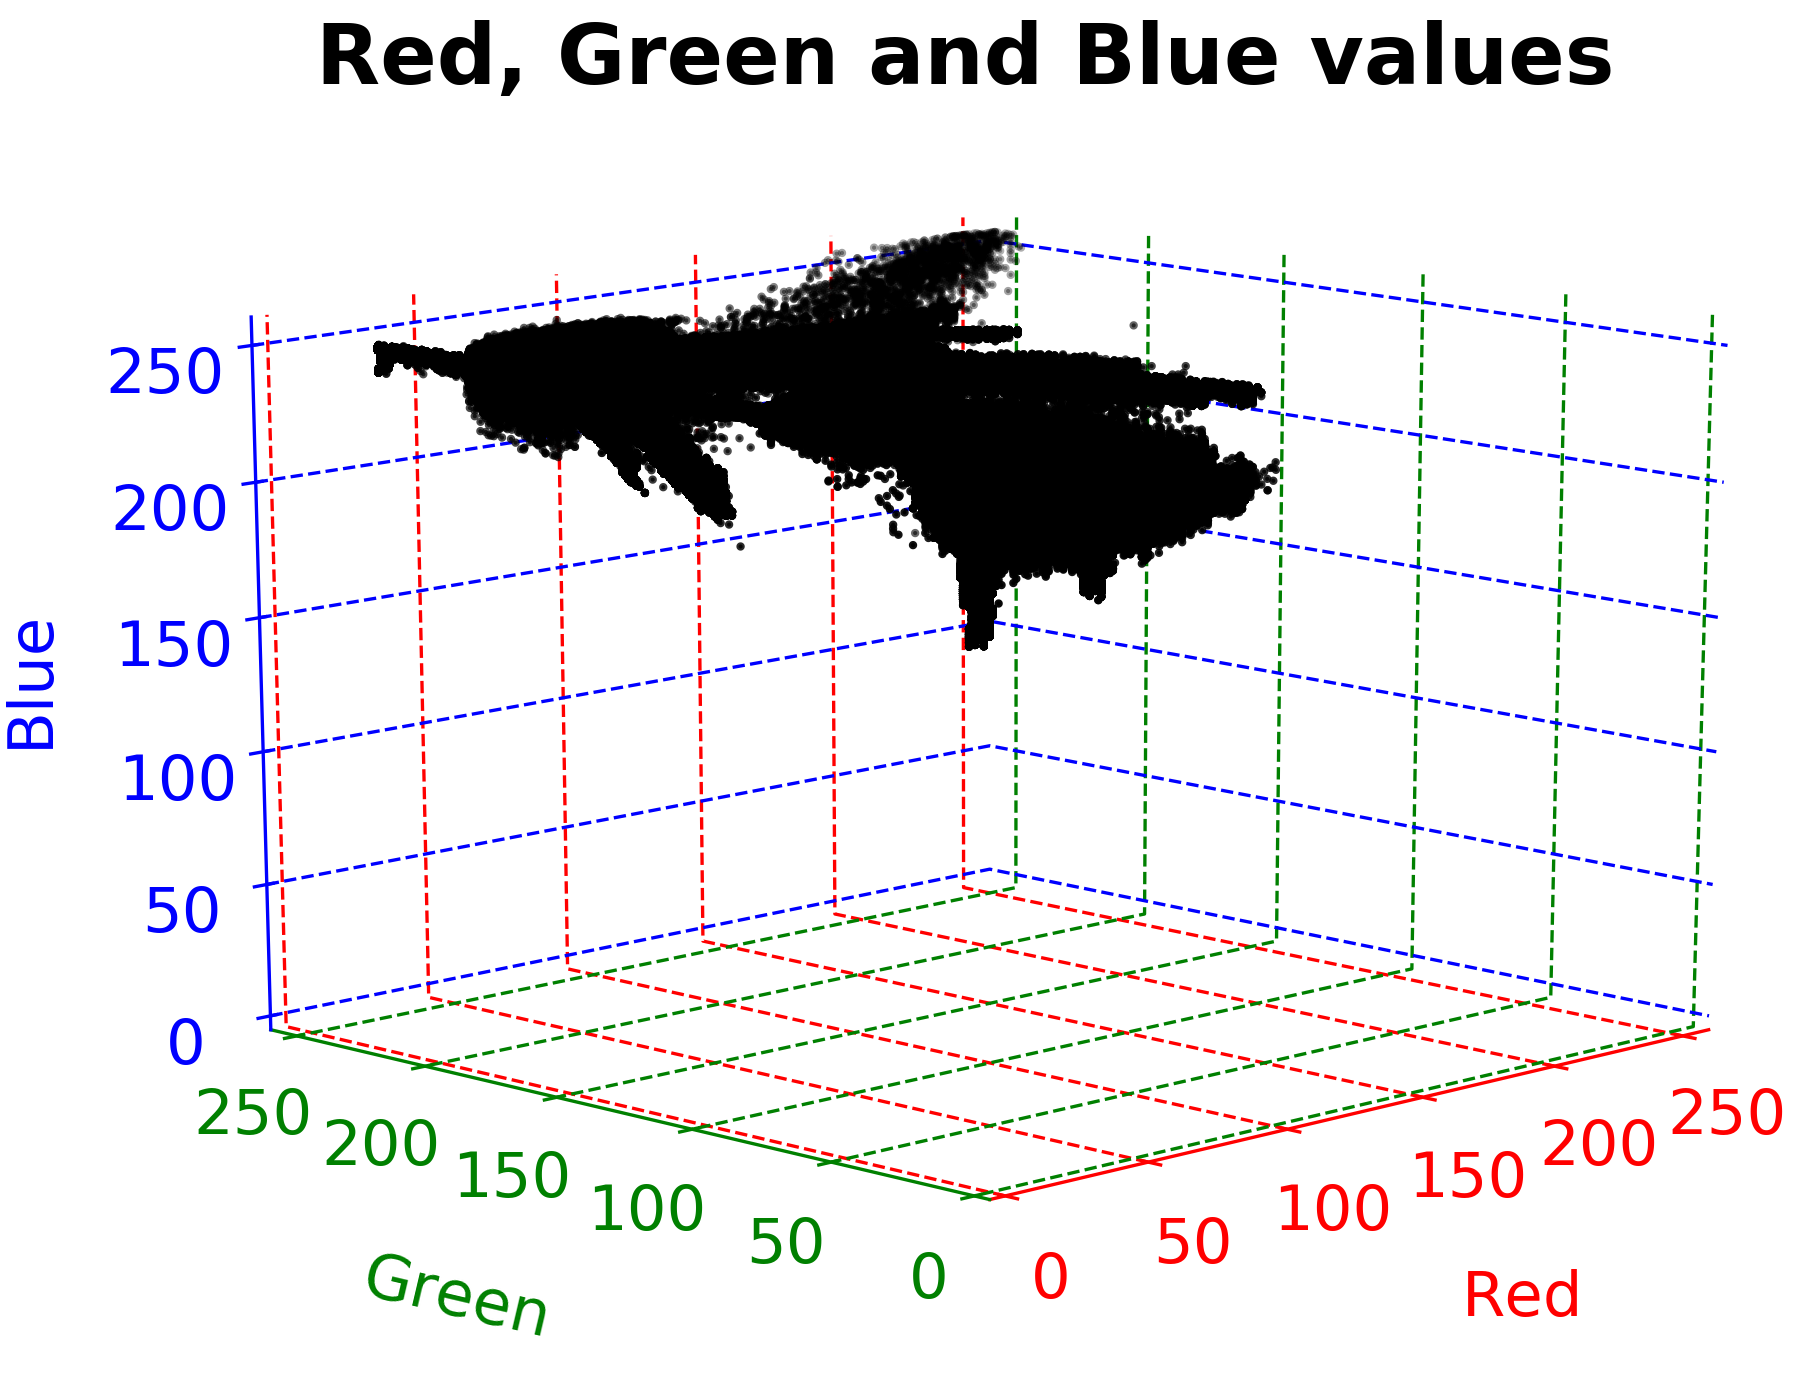
\includegraphics[width=0.9\textwidth]{img/rgbBlue.png}
		\captionsetup{width=0.9\textwidth}
		\captionof{figure}{RGB plot voor de kleur blauw.}
		\label{rgbBluePlot}
	\end{minipage}%	
	\begin{minipage}{0.5\textwidth}
		\centering
		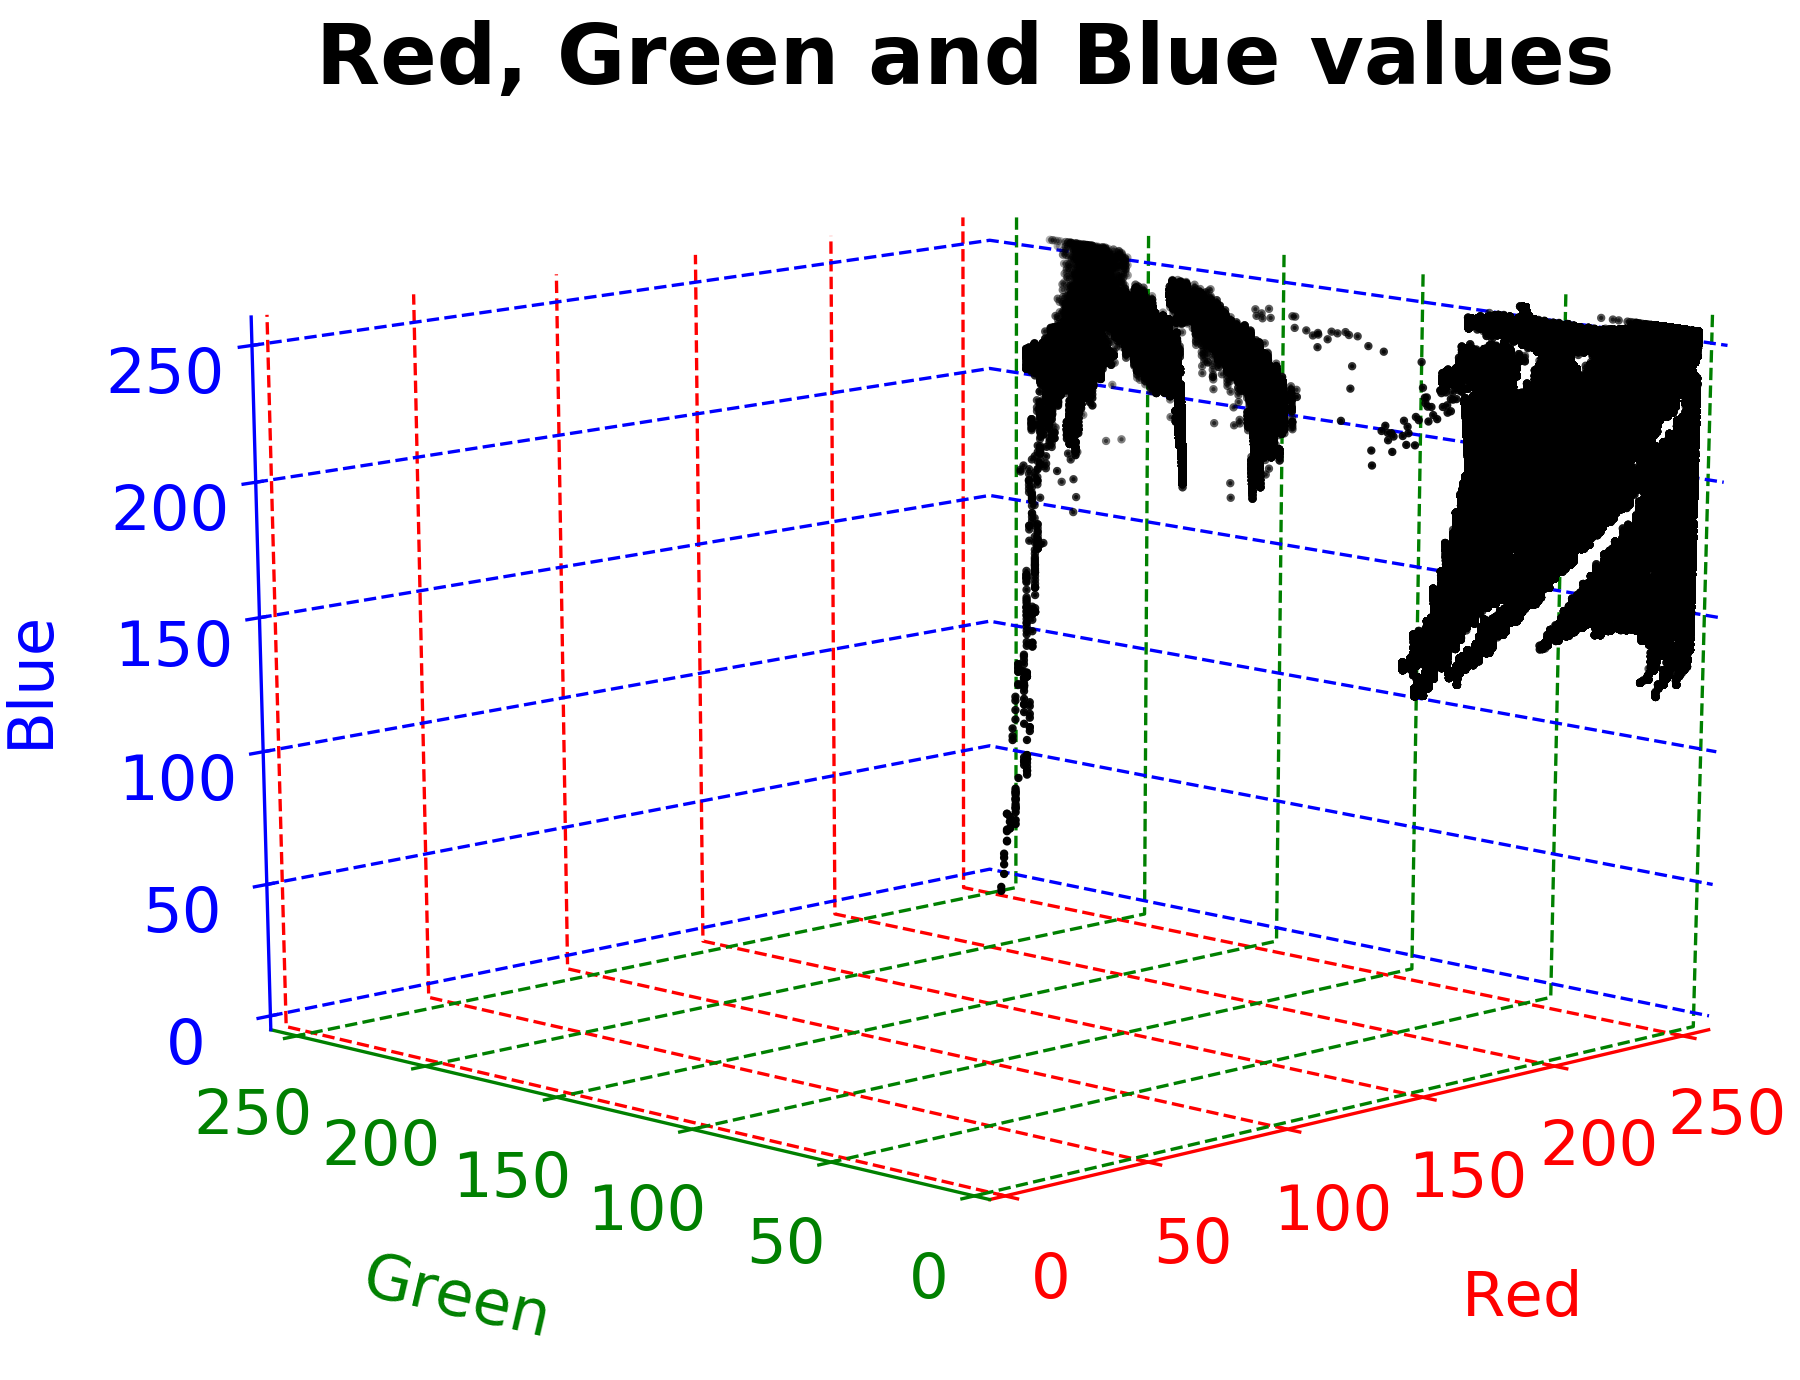
\includegraphics[width=0.9\textwidth]{img/rgbPink.png}
		\captionsetup{width=0.9\textwidth}
		\captionof{figure}{RGB plot voor de kleur magenta.}
		\label{rgbPinkPlot}
	\end{minipage}
\end{figure}

\subsection{Histogrammen}

\begin{figure}[h!]
	\centering
	\begin{minipage}{0.5\textwidth}
		\centering
		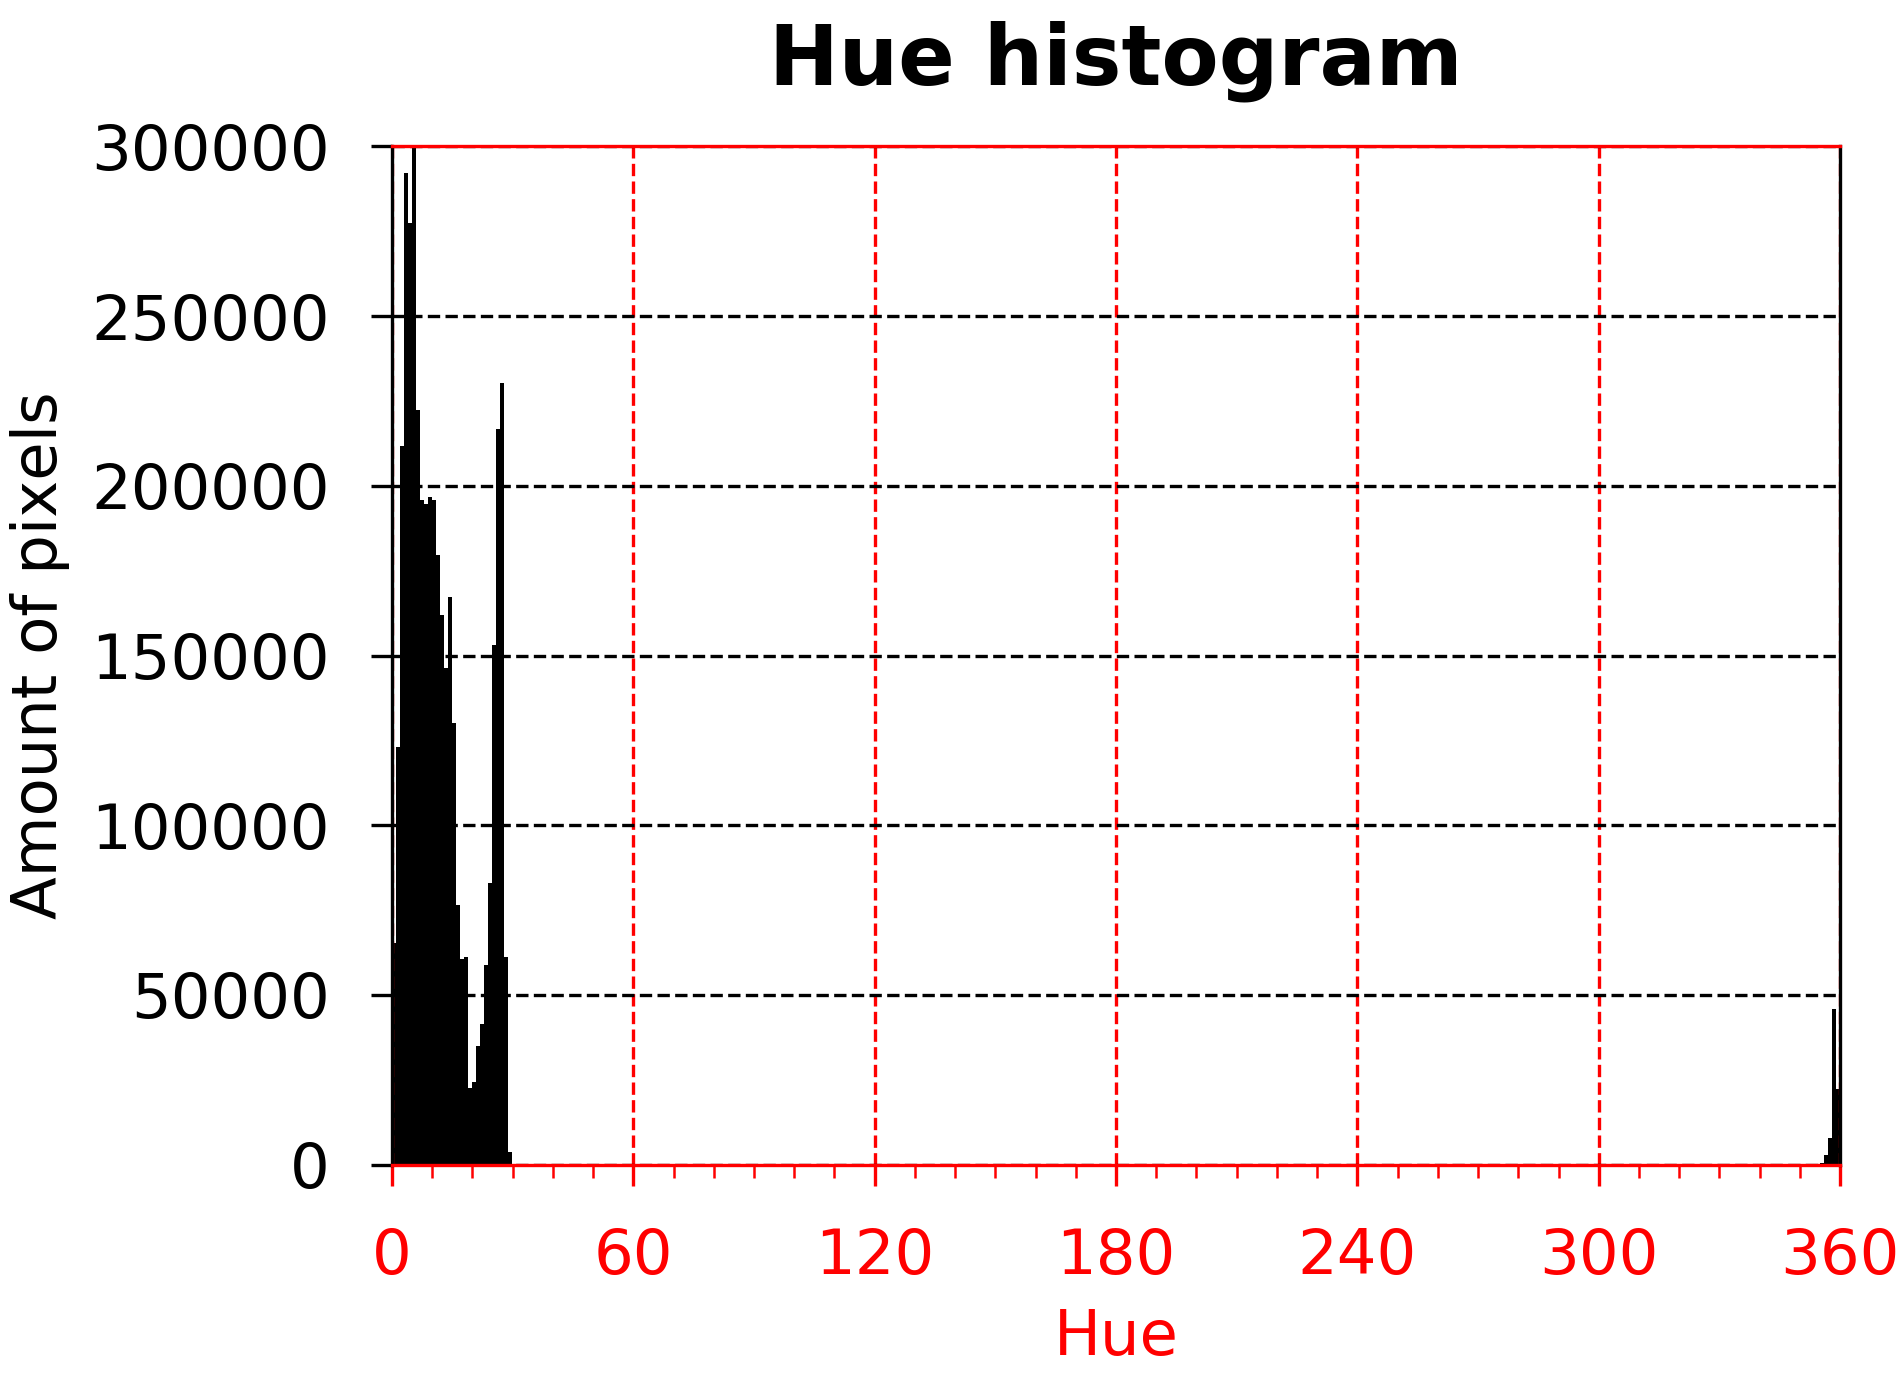
\includegraphics[width=0.9\textwidth]{img/hueHistRed.png}
		\captionsetup{width=0.9\textwidth}
		\captionof{figure}{Histogram van de tint in functie van het aantal waargenomen pixels voor de kleur rood.}
		\label{histRed}
	\end{minipage}%
	\begin{minipage}{0.5\textwidth}
		\centering
		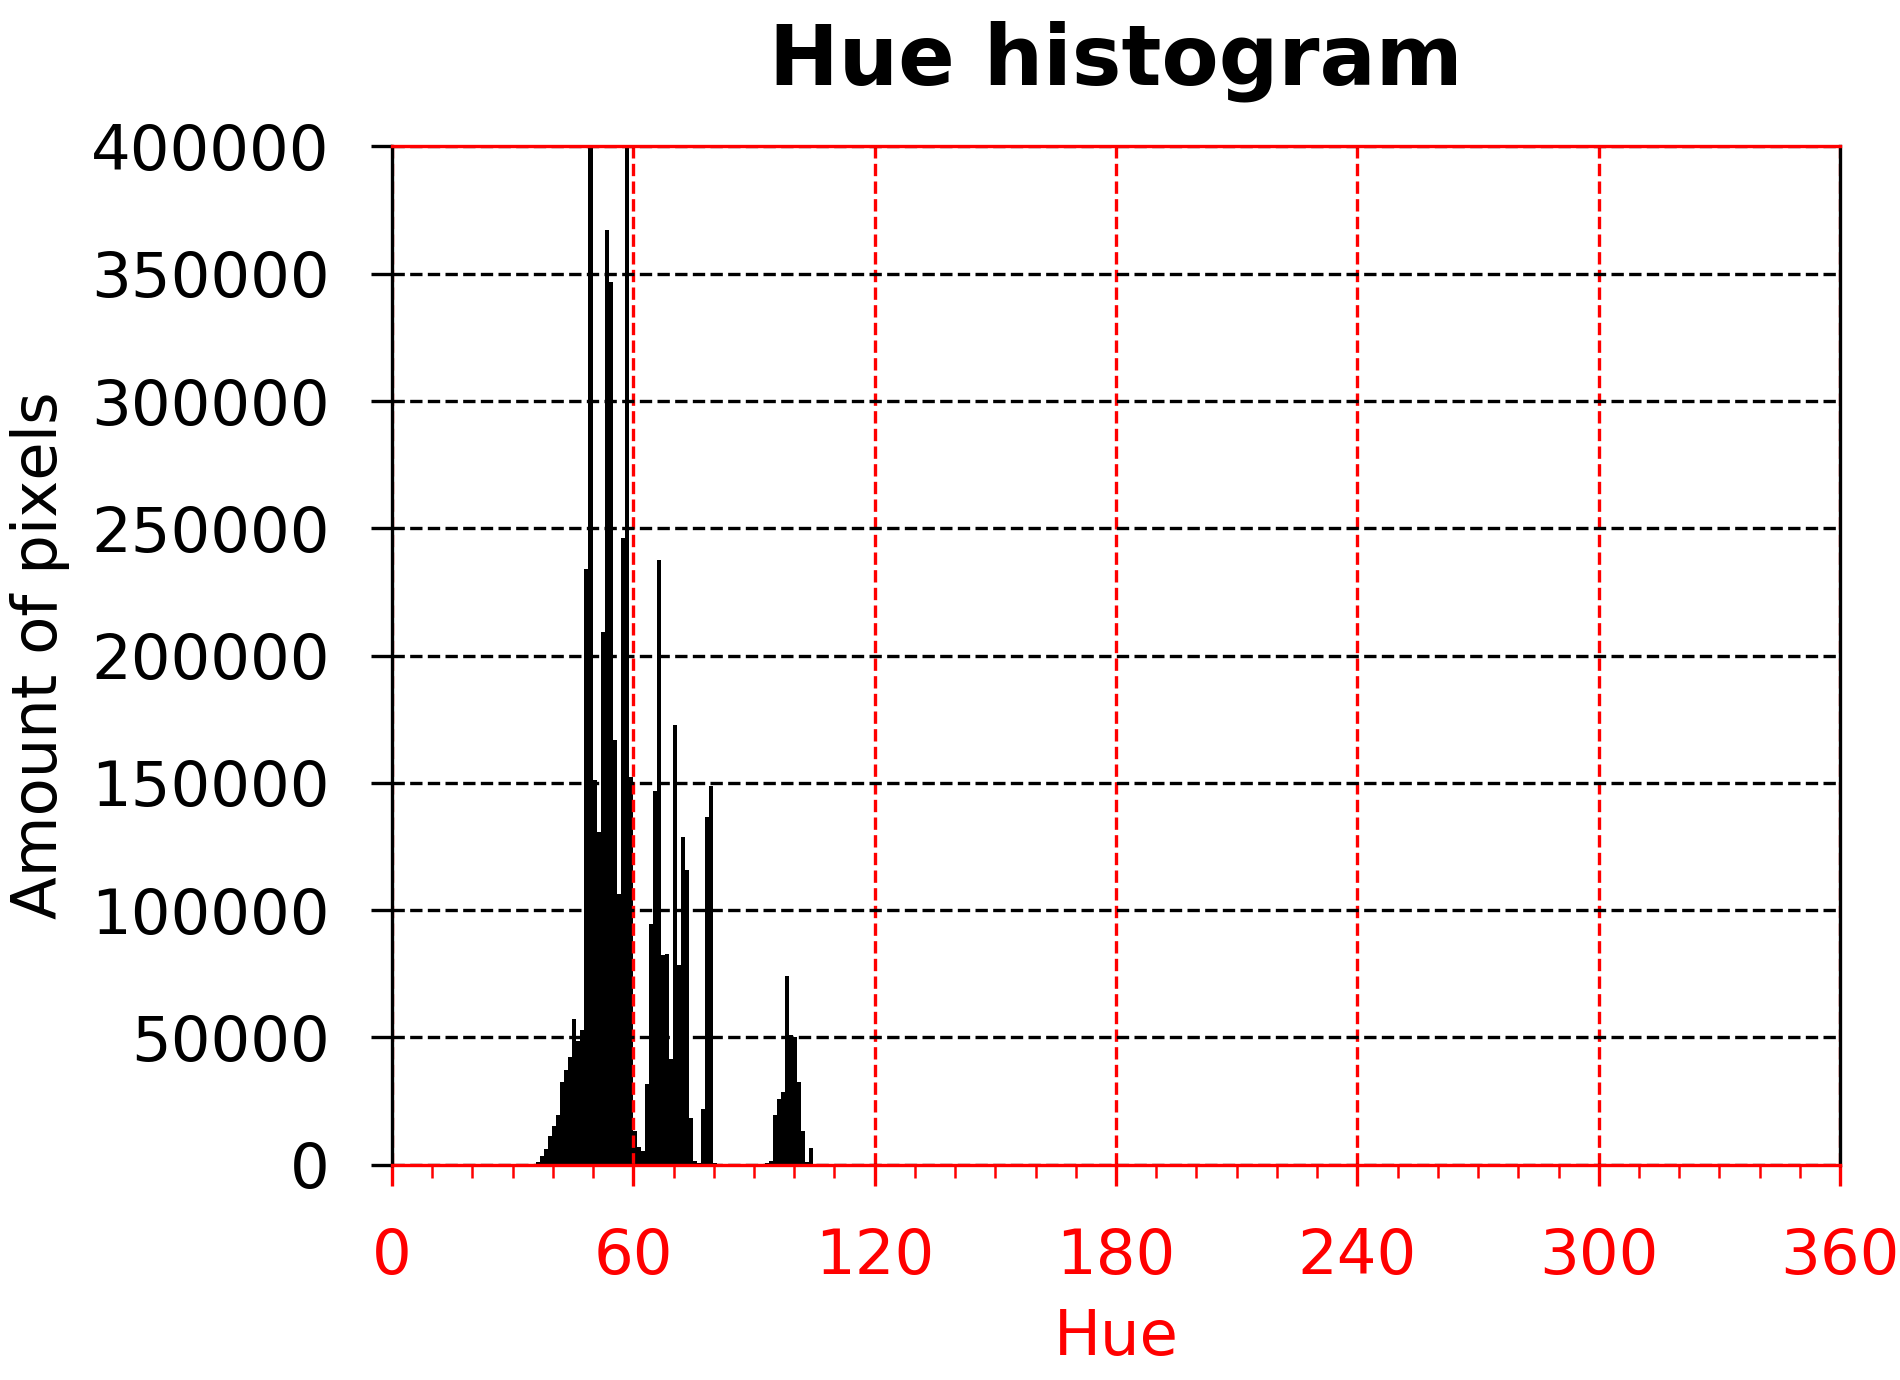
\includegraphics[width=0.9\textwidth]{img/hueHistYellow.png}
		\captionsetup{width=0.9\textwidth}
		\captionof{figure}{Histogram van de tint in functie van het aantal waargenomen pixels voor de kleur geel.}
	\label{histYellow}
	\end{minipage}
\end{figure}

\vspace{1mm}

\begin{figure}[h!]
	\centering
	\begin{minipage}{0.5\textwidth}
		\centering
		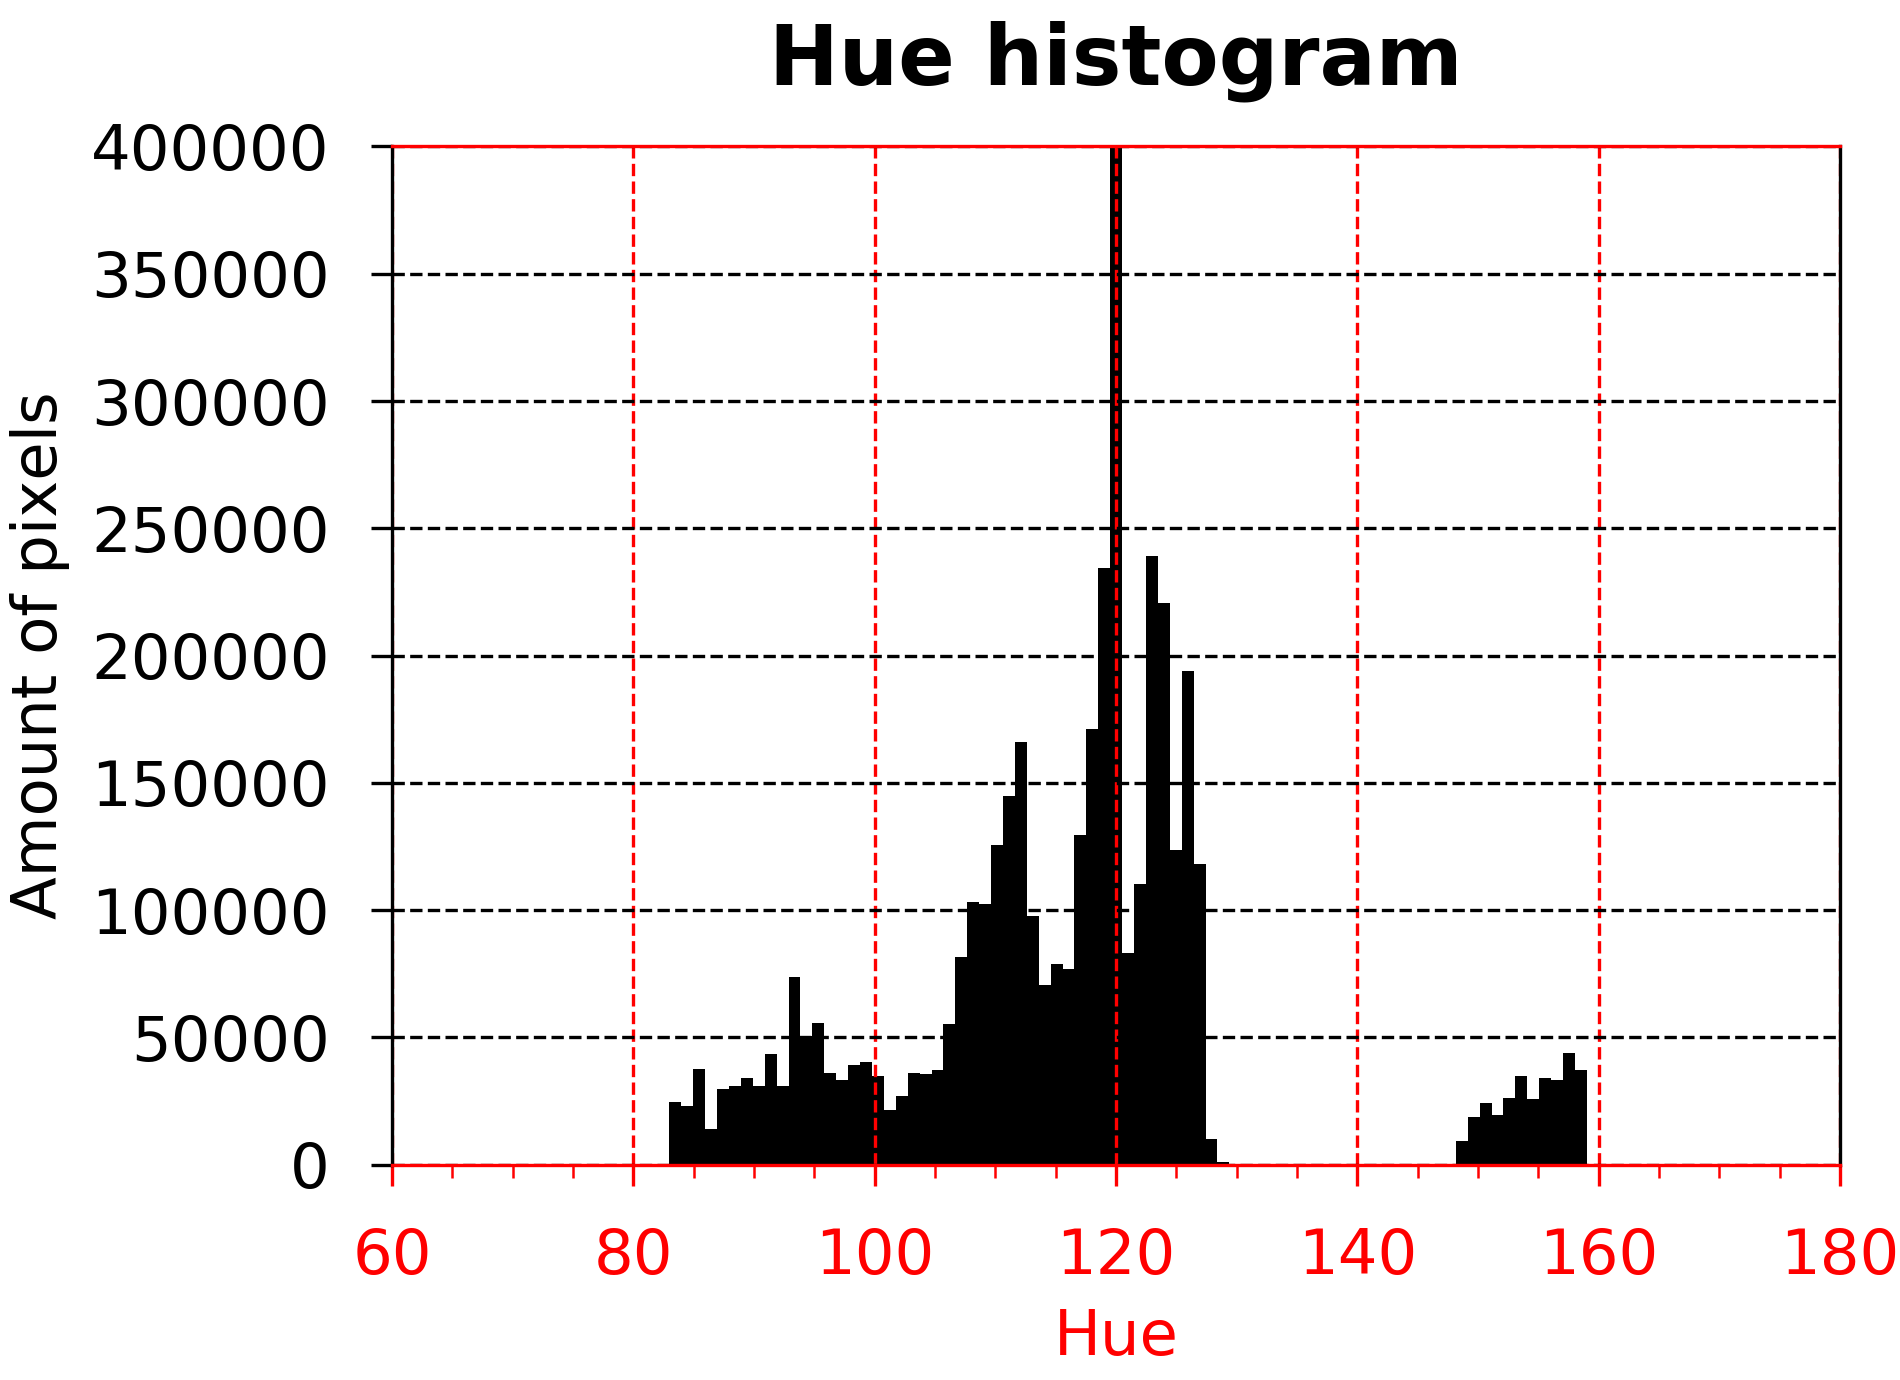
\includegraphics[width=0.9\textwidth]{img/hueHistGreen.png}
		\captionsetup{width=0.9\textwidth}
		\captionof{figure}{Histogram van de tint in functie van het aantal waargenomen pixels voor de kleur groen.}
		\label{histGreen}
	\end{minipage}%
	\begin{minipage}{0.5\textwidth}
		\centering
		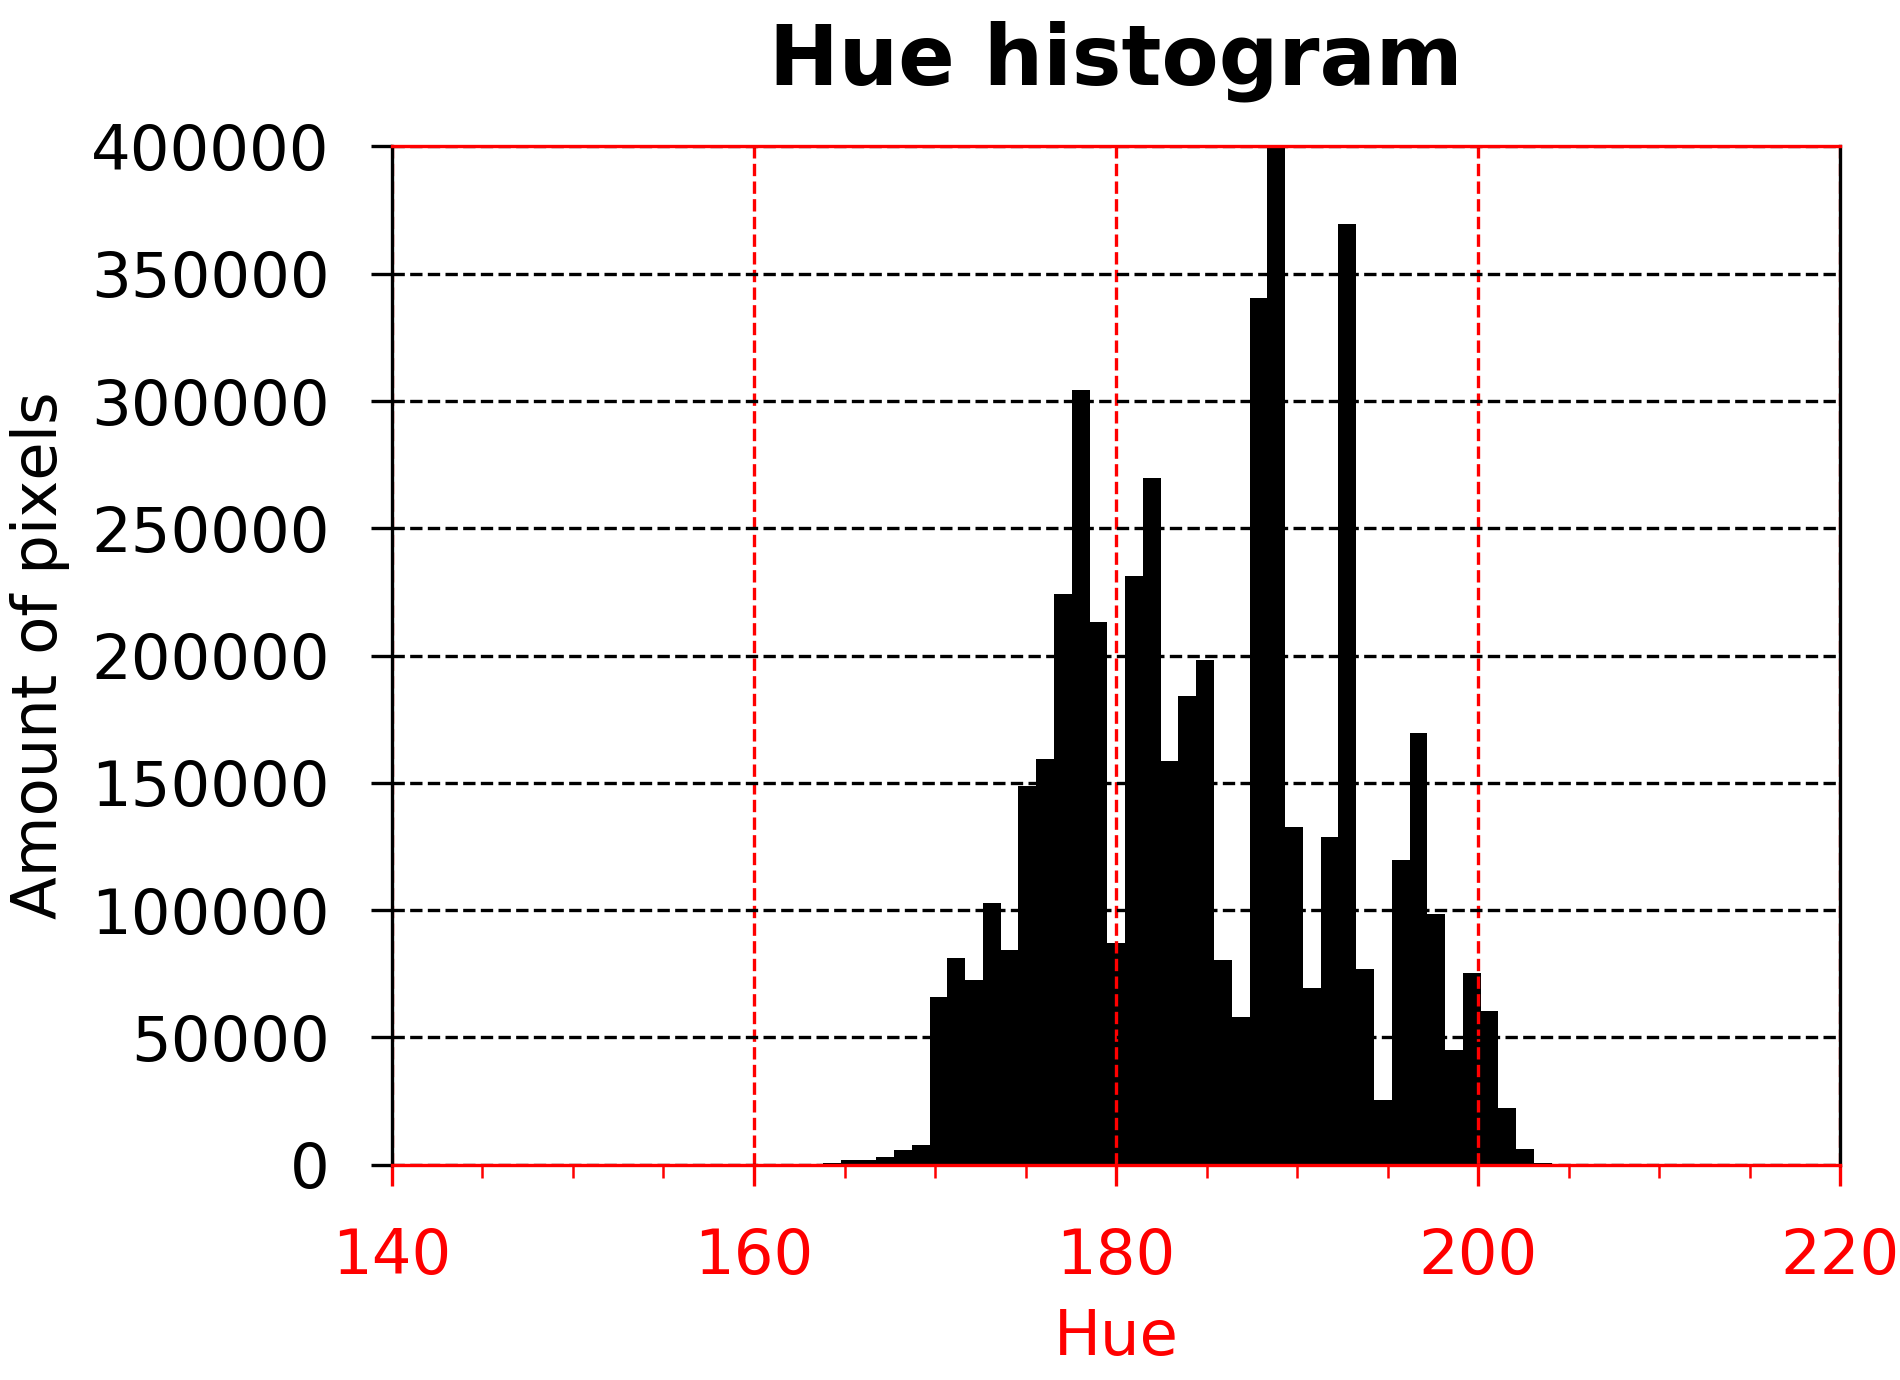
\includegraphics[width=0.9\textwidth]{img/hueHistBlueGreen.png}
		\captionsetup{width=0.9\textwidth}
		\captionof{figure}{Histogram van de tint in functie van het aantal waargenomen pixels voor de kleur cyaan.}
	\label{histBluegreen}
	\end{minipage}
\end{figure}

\vspace{1mm}

\begin{figure}[h!]
	\centering
	\begin{minipage}{0.5\textwidth}
		\centering
		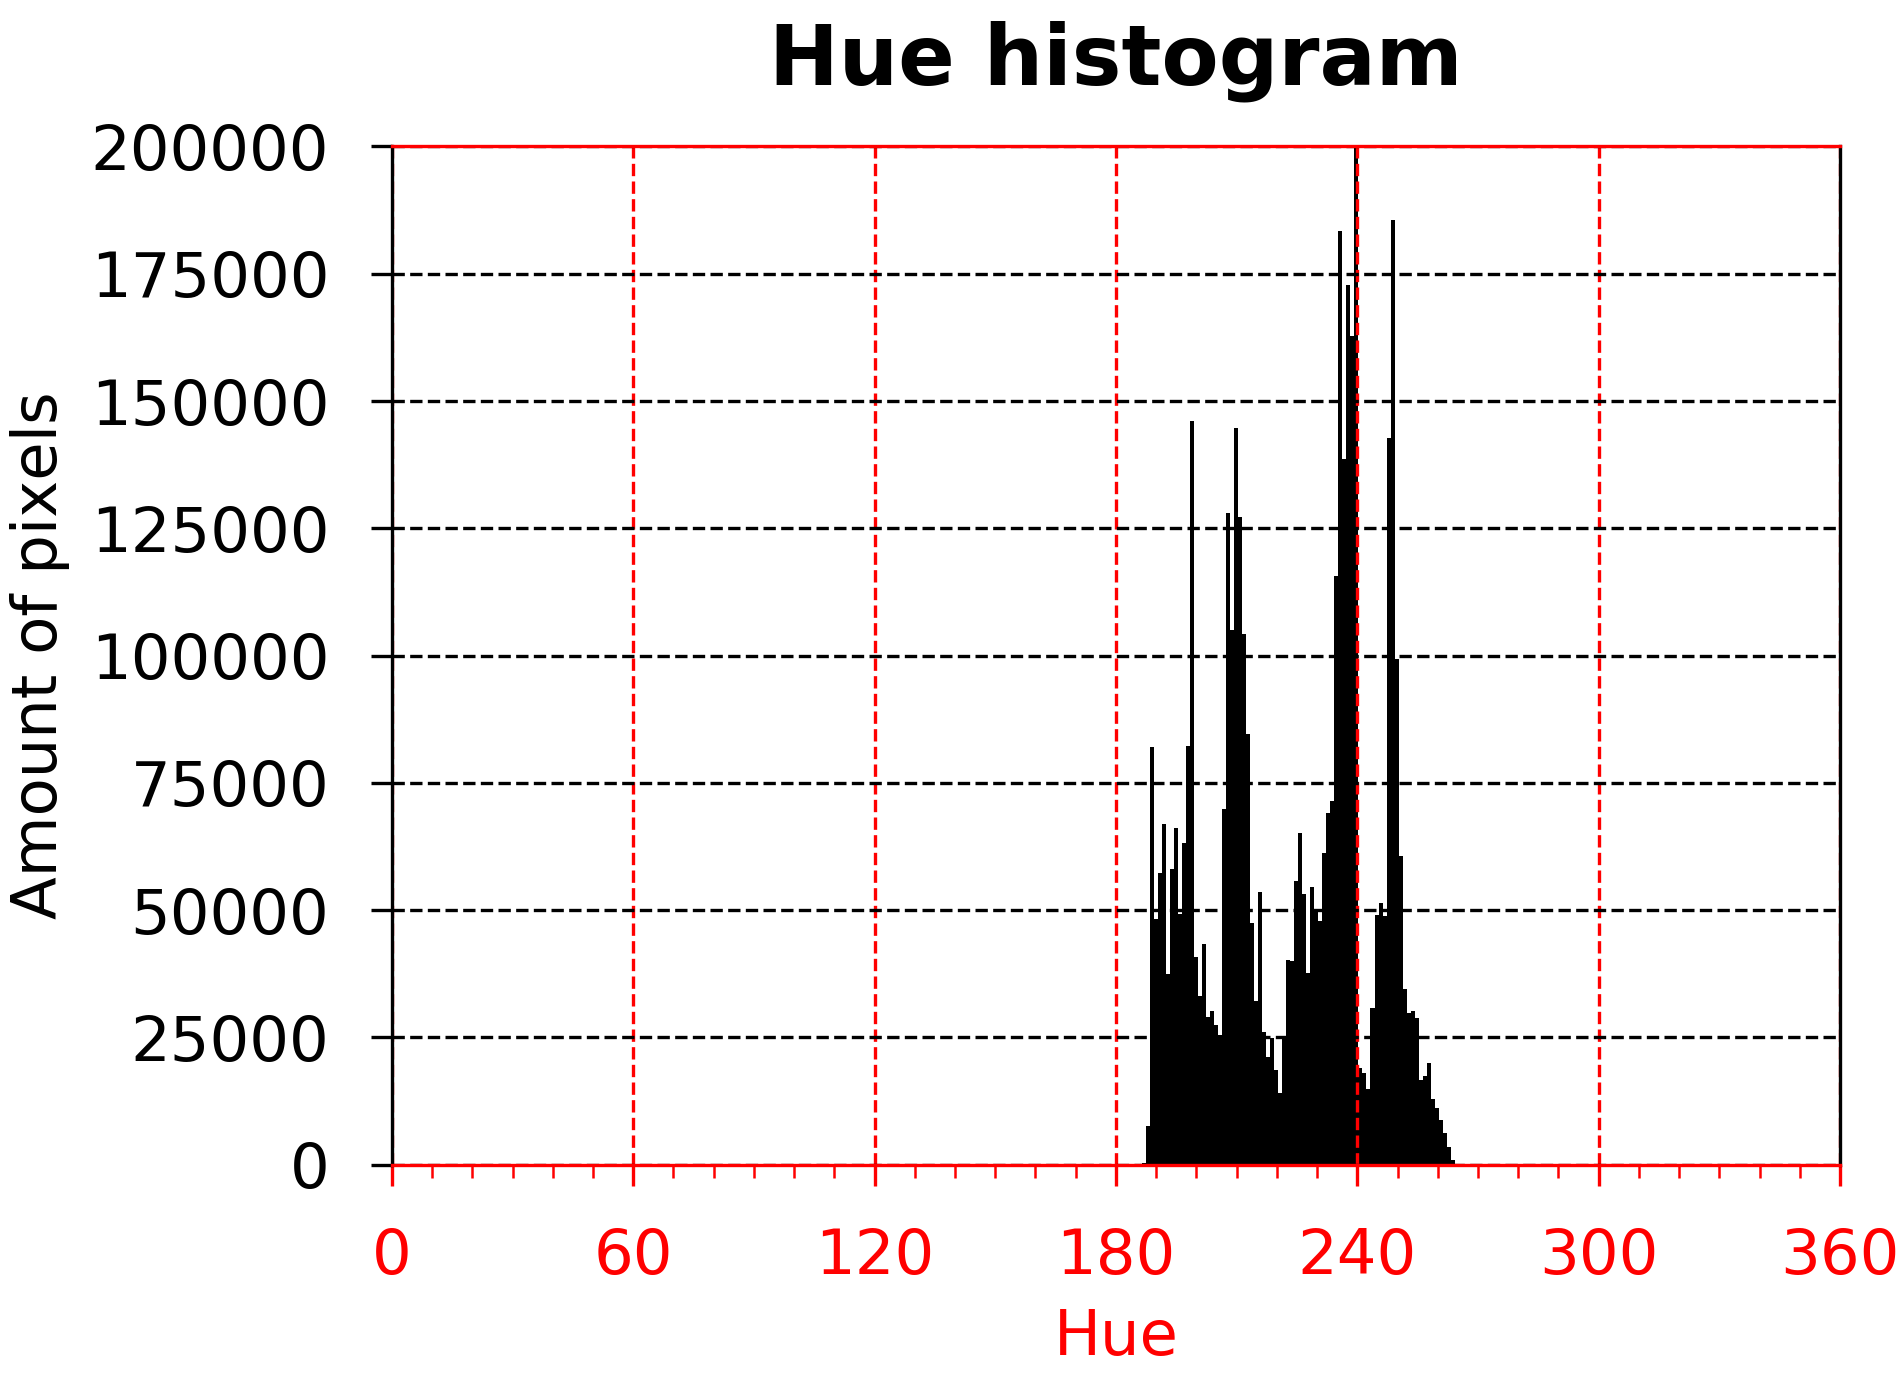
\includegraphics[width=0.9\textwidth]{img/hueHistBlue.png}
		\captionsetup{width=0.9\textwidth}
		\captionof{figure}{Histogram van de tint in functie van het aantal waargenomen pixels voor de kleur blauw.}
		\label{histBlue}
	\end{minipage}%
	\begin{minipage}{0.5\textwidth}
		\centering
		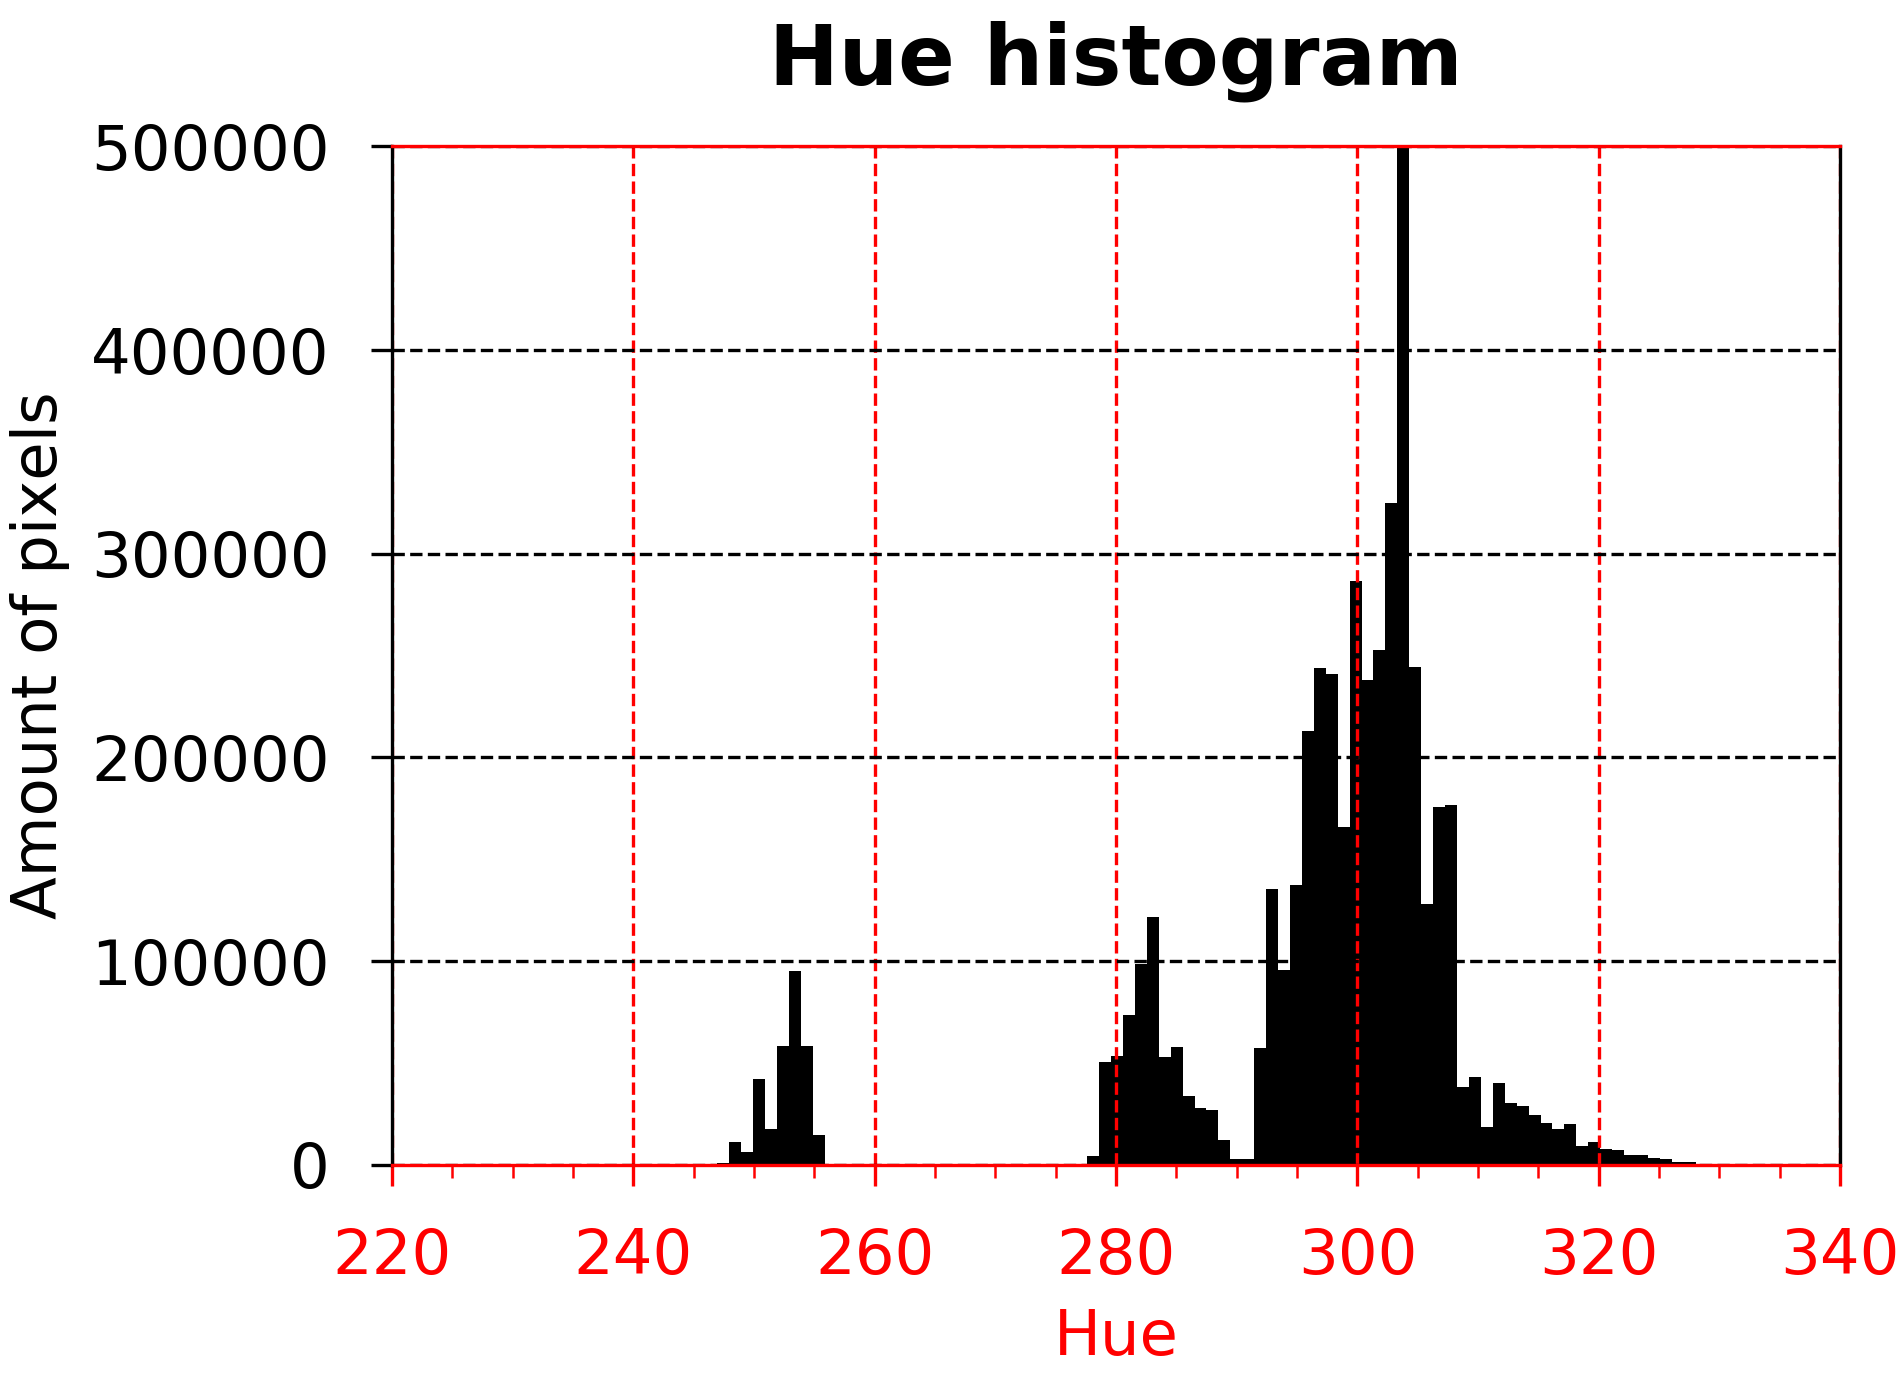
\includegraphics[width=0.9\textwidth]{img/hueHistPink.png}
		\captionsetup{width=0.9\textwidth}
		\captionof{figure}{Histogram van de tint in functie van het aantal waargenomen pixels voor de kleur magenta.}
	\label{histPink}
	\end{minipage}
\end{figure}

\subsection{HSL plots}

\subsubsection{3D}

\begin{figure}[h!]
	\centering
	\begin{minipage}{0.5\textwidth}
		\centering
		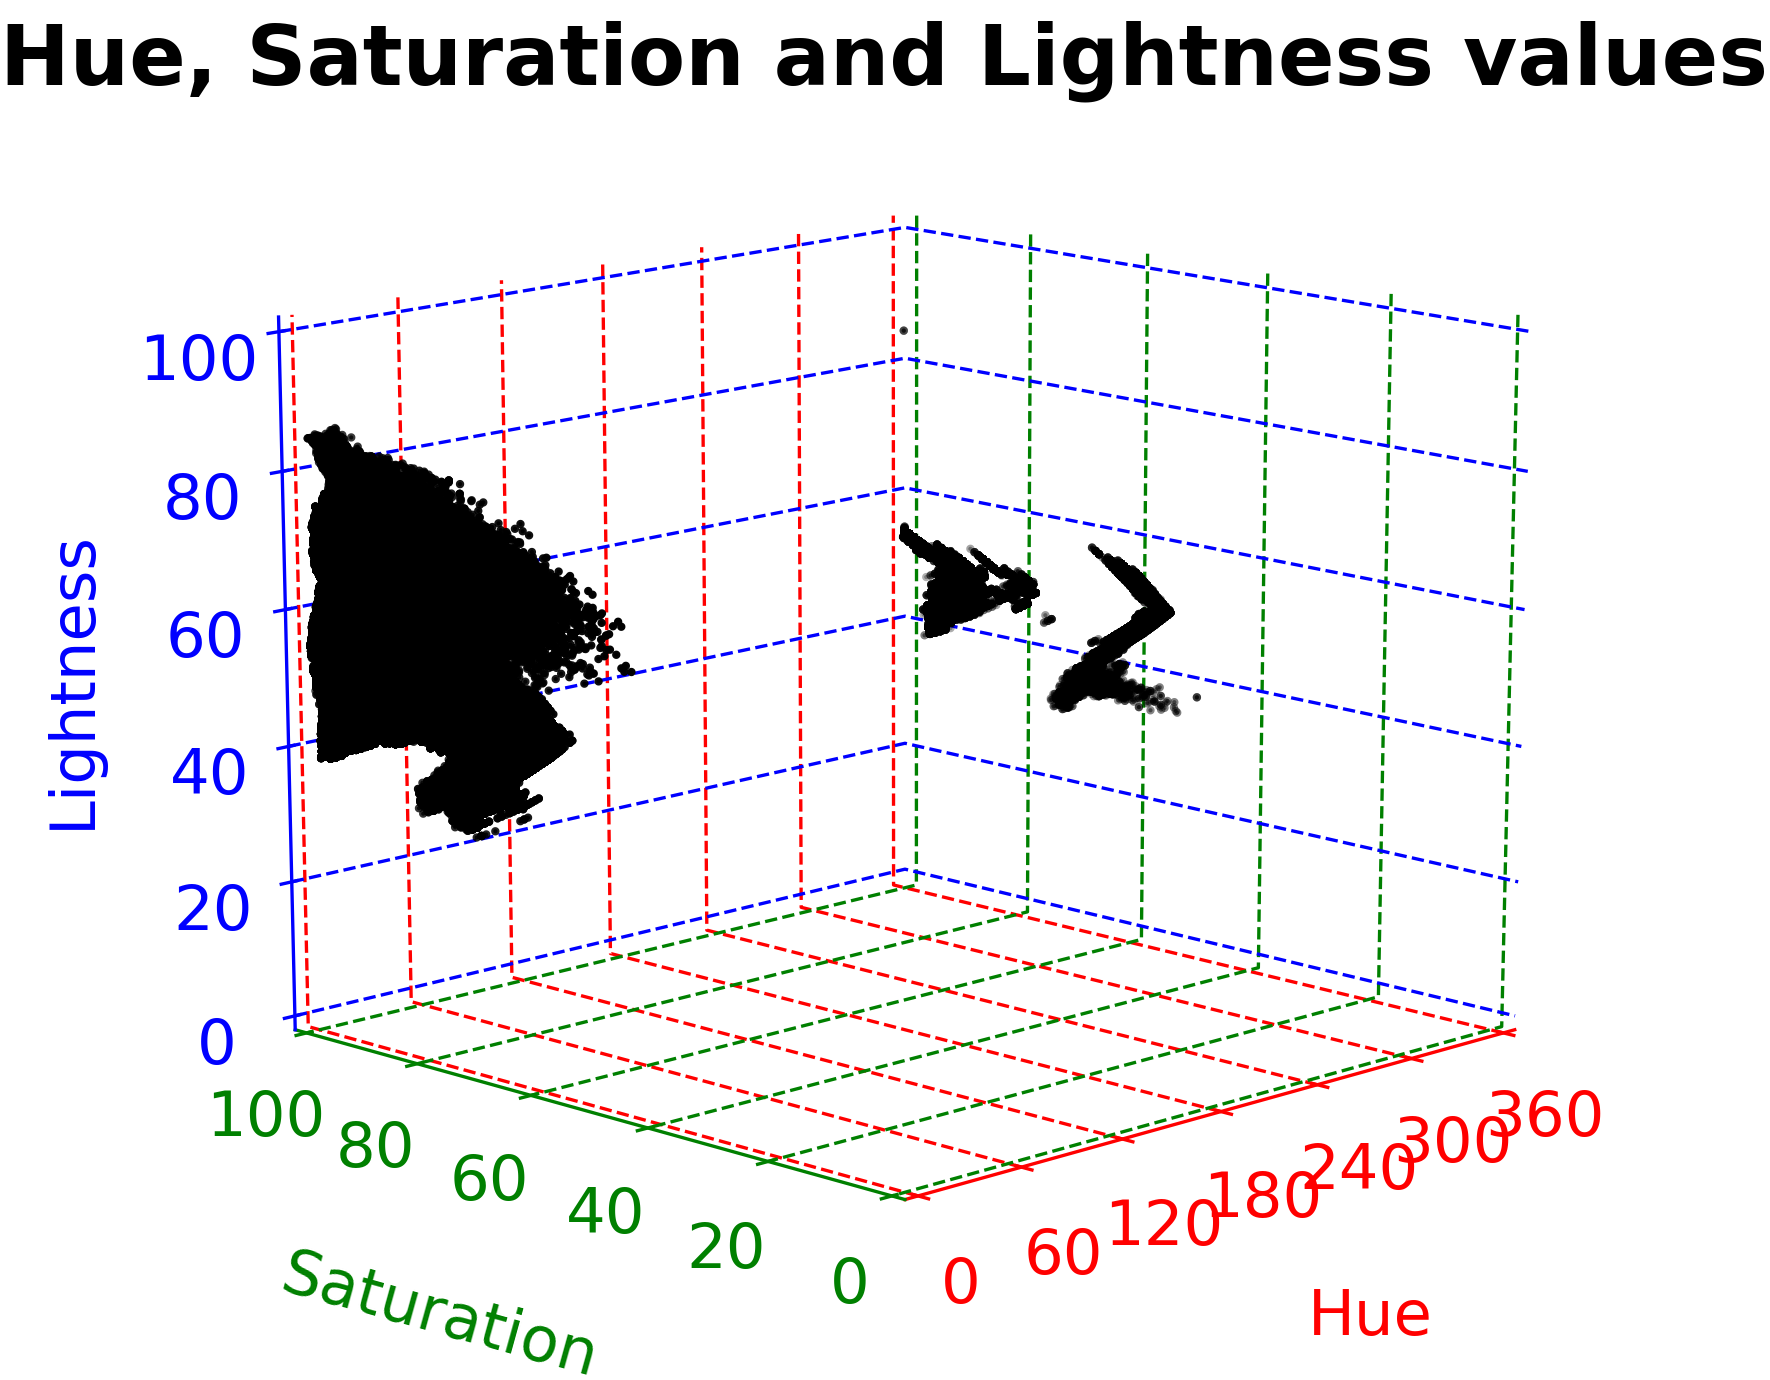
\includegraphics[width=0.9\textwidth]{img/hsl3DRed.png}
		\captionsetup{width=0.9\textwidth}
		\captionof{figure}{HSL plot voor de kleur rood.}
		\label{hsl3DRedPlot}
	\end{minipage}%
	\begin{minipage}{0.5\textwidth}
		\centering
		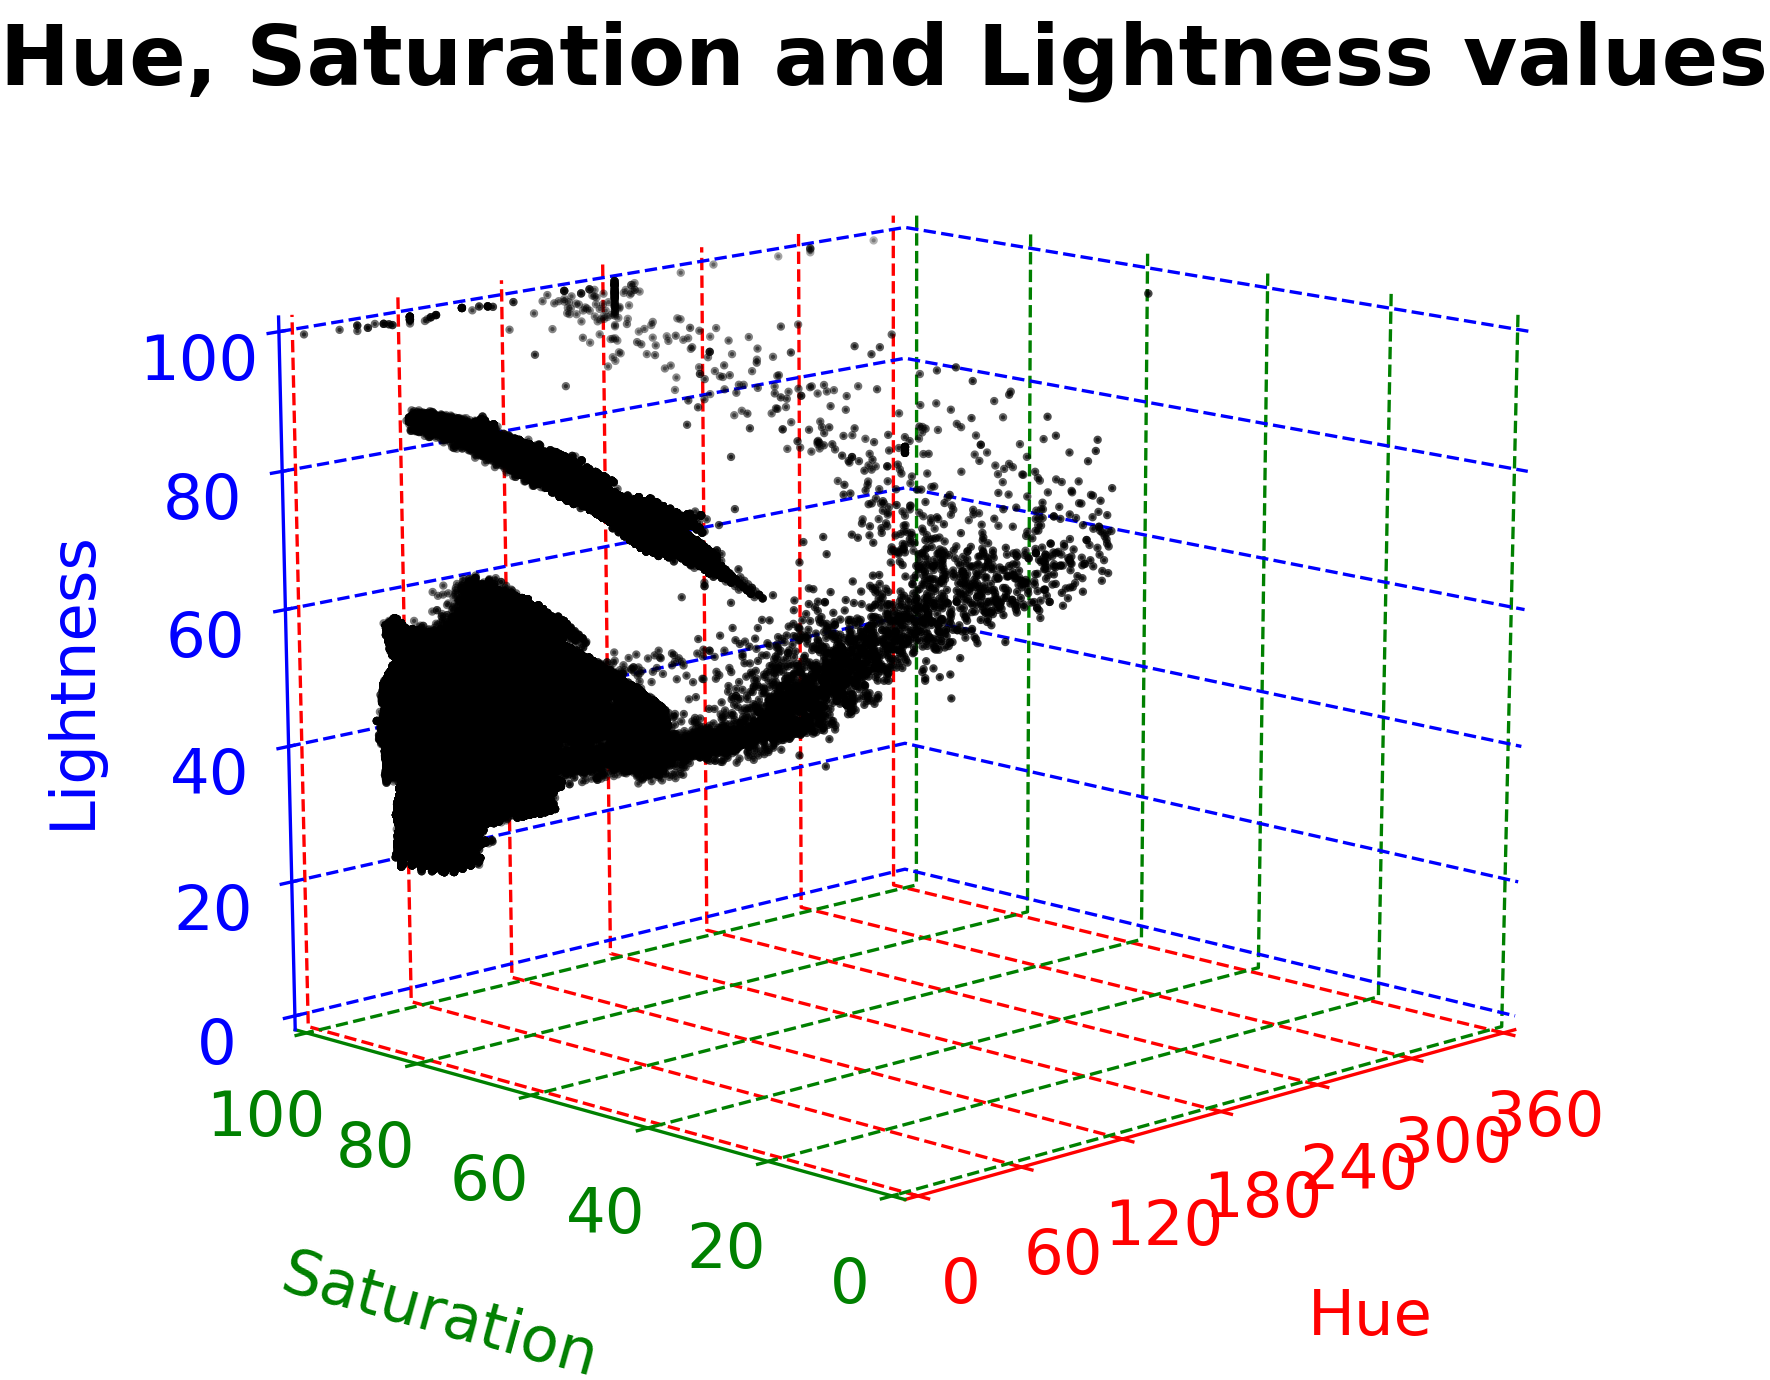
\includegraphics[width=0.9\textwidth]{img/hsl3DYellow.png}
		\captionsetup{width=0.9\textwidth}
		\captionof{figure}{HSL plot voor de kleur geel.}
		\label{hsl3DYellowPlot}
	\end{minipage}
\end{figure}

\vspace{5mm}

\begin{figure}[h!]
	\centering
	\begin{minipage}{0.5\textwidth}
		\centering
		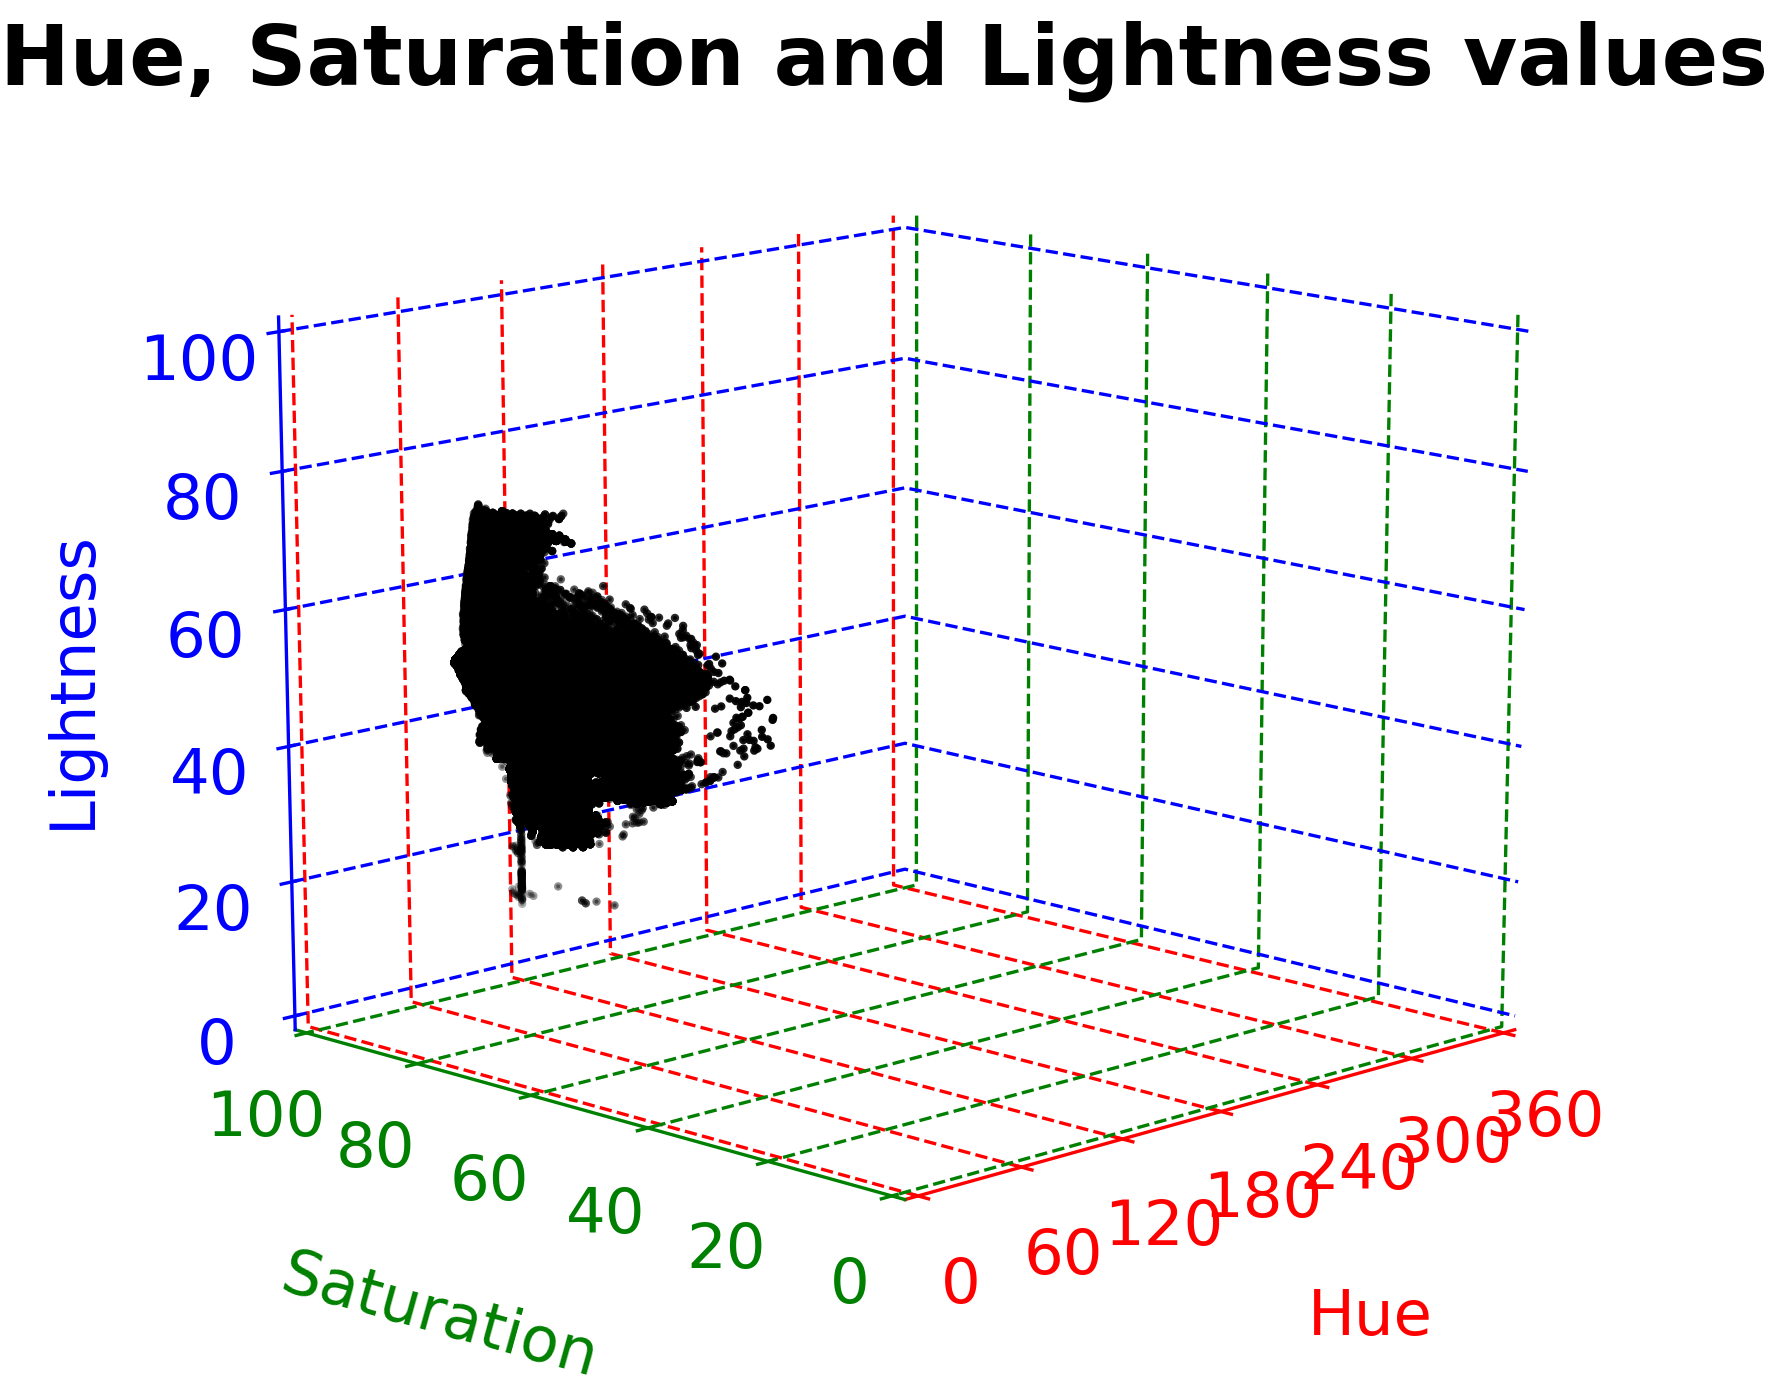
\includegraphics[width=0.9\textwidth]{img/hsl3DGreen.png}
		\captionsetup{width=0.9\textwidth}
		\captionof{figure}{HSL plot voor de kleur groen.}
		\label{hsl3DGreenPlot}
	\end{minipage}%
	\begin{minipage}{0.5\textwidth}
		\centering
		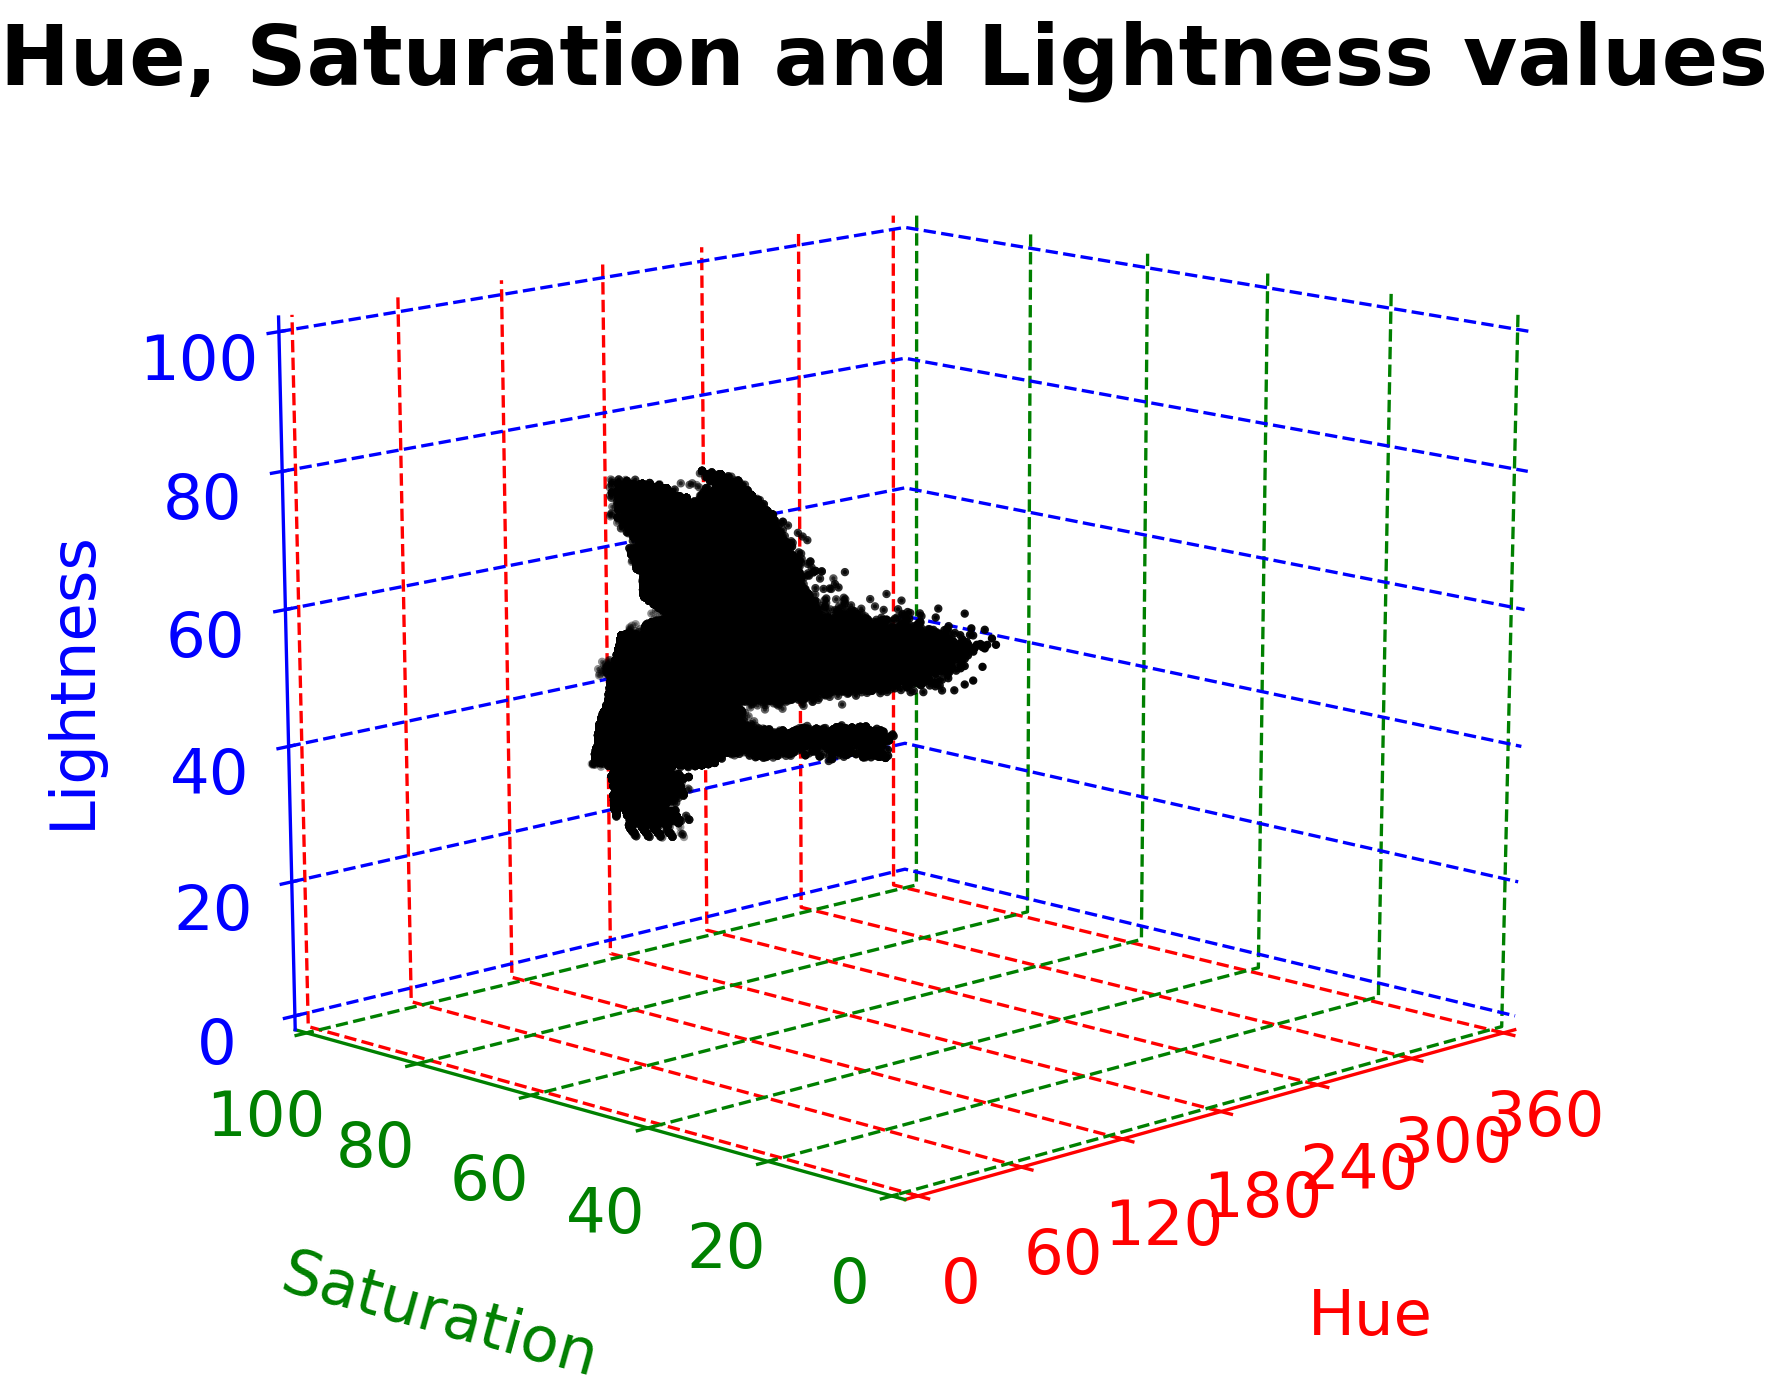
\includegraphics[width=0.9\textwidth]{img/hsl3DBlueGreen.png}
		\captionsetup{width=0.9\textwidth}
		\captionof{figure}{HSL plot voor de kleur cyaan.}
		\label{hsl3DBlueGreenPlot}
	\end{minipage}
\end{figure}

\vspace{5mm}

\begin{figure}[h!]
	\centering
	\begin{minipage}{0.5\textwidth}
		\centering
		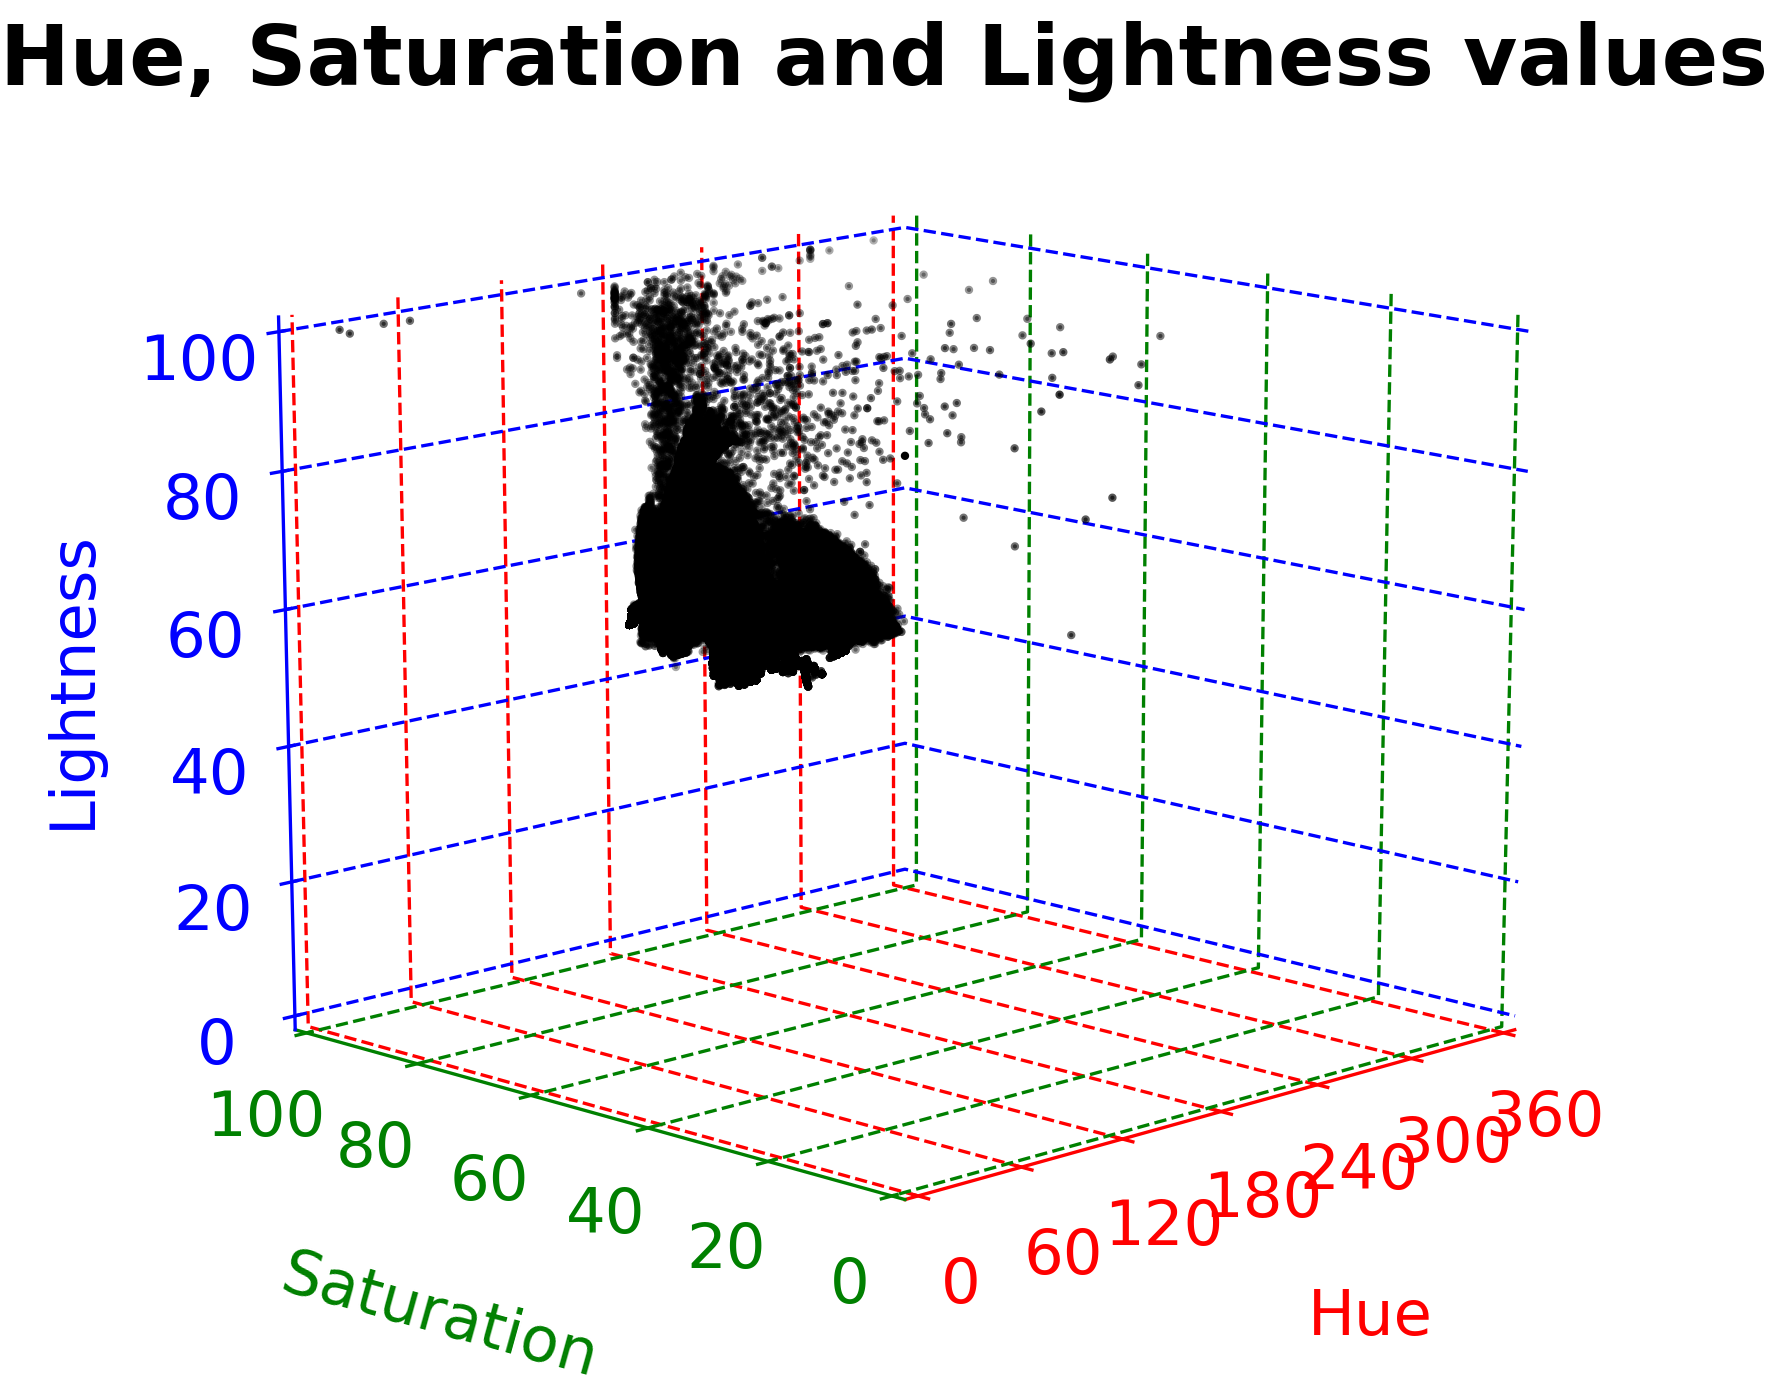
\includegraphics[width=0.9\textwidth]{img/hsl3DBlue.png}
		\captionsetup{width=0.9\textwidth}
		\captionof{figure}{HSL plot voor de kleur blauw.}
		\label{hsl3DBluePlot}
	\end{minipage}%	
	\begin{minipage}{0.5\textwidth}
		\centering
		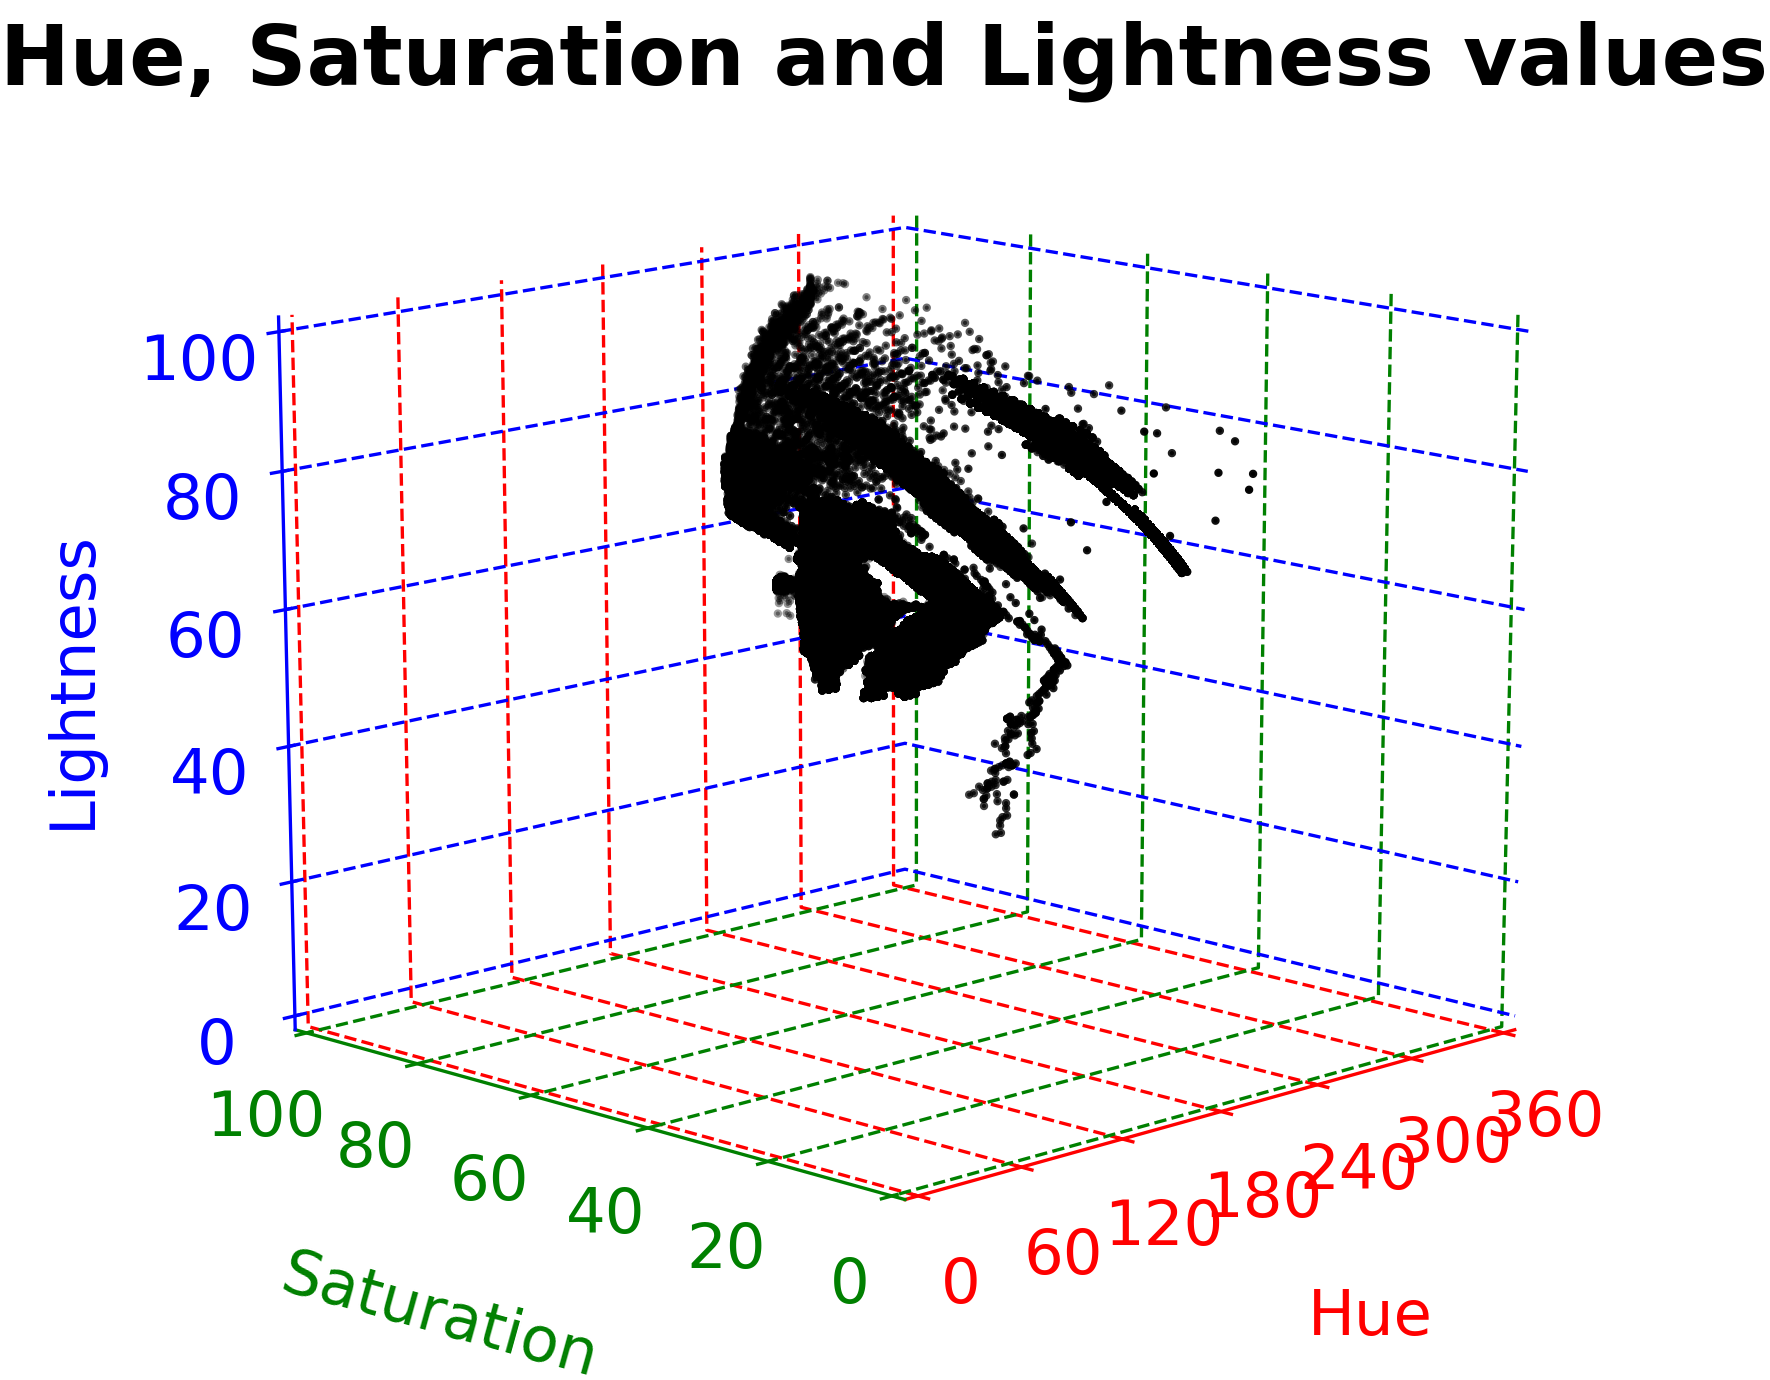
\includegraphics[width=0.9\textwidth]{img/hsl3DPink.png}
		\captionsetup{width=0.9\textwidth}
		\captionof{figure}{HSL plot voor de kleur magenta.}
		\label{hsl3DPinkPlot}
	\end{minipage}
\end{figure}

\subsubsection{2D}

\begin{figure}[h!]
	\center
	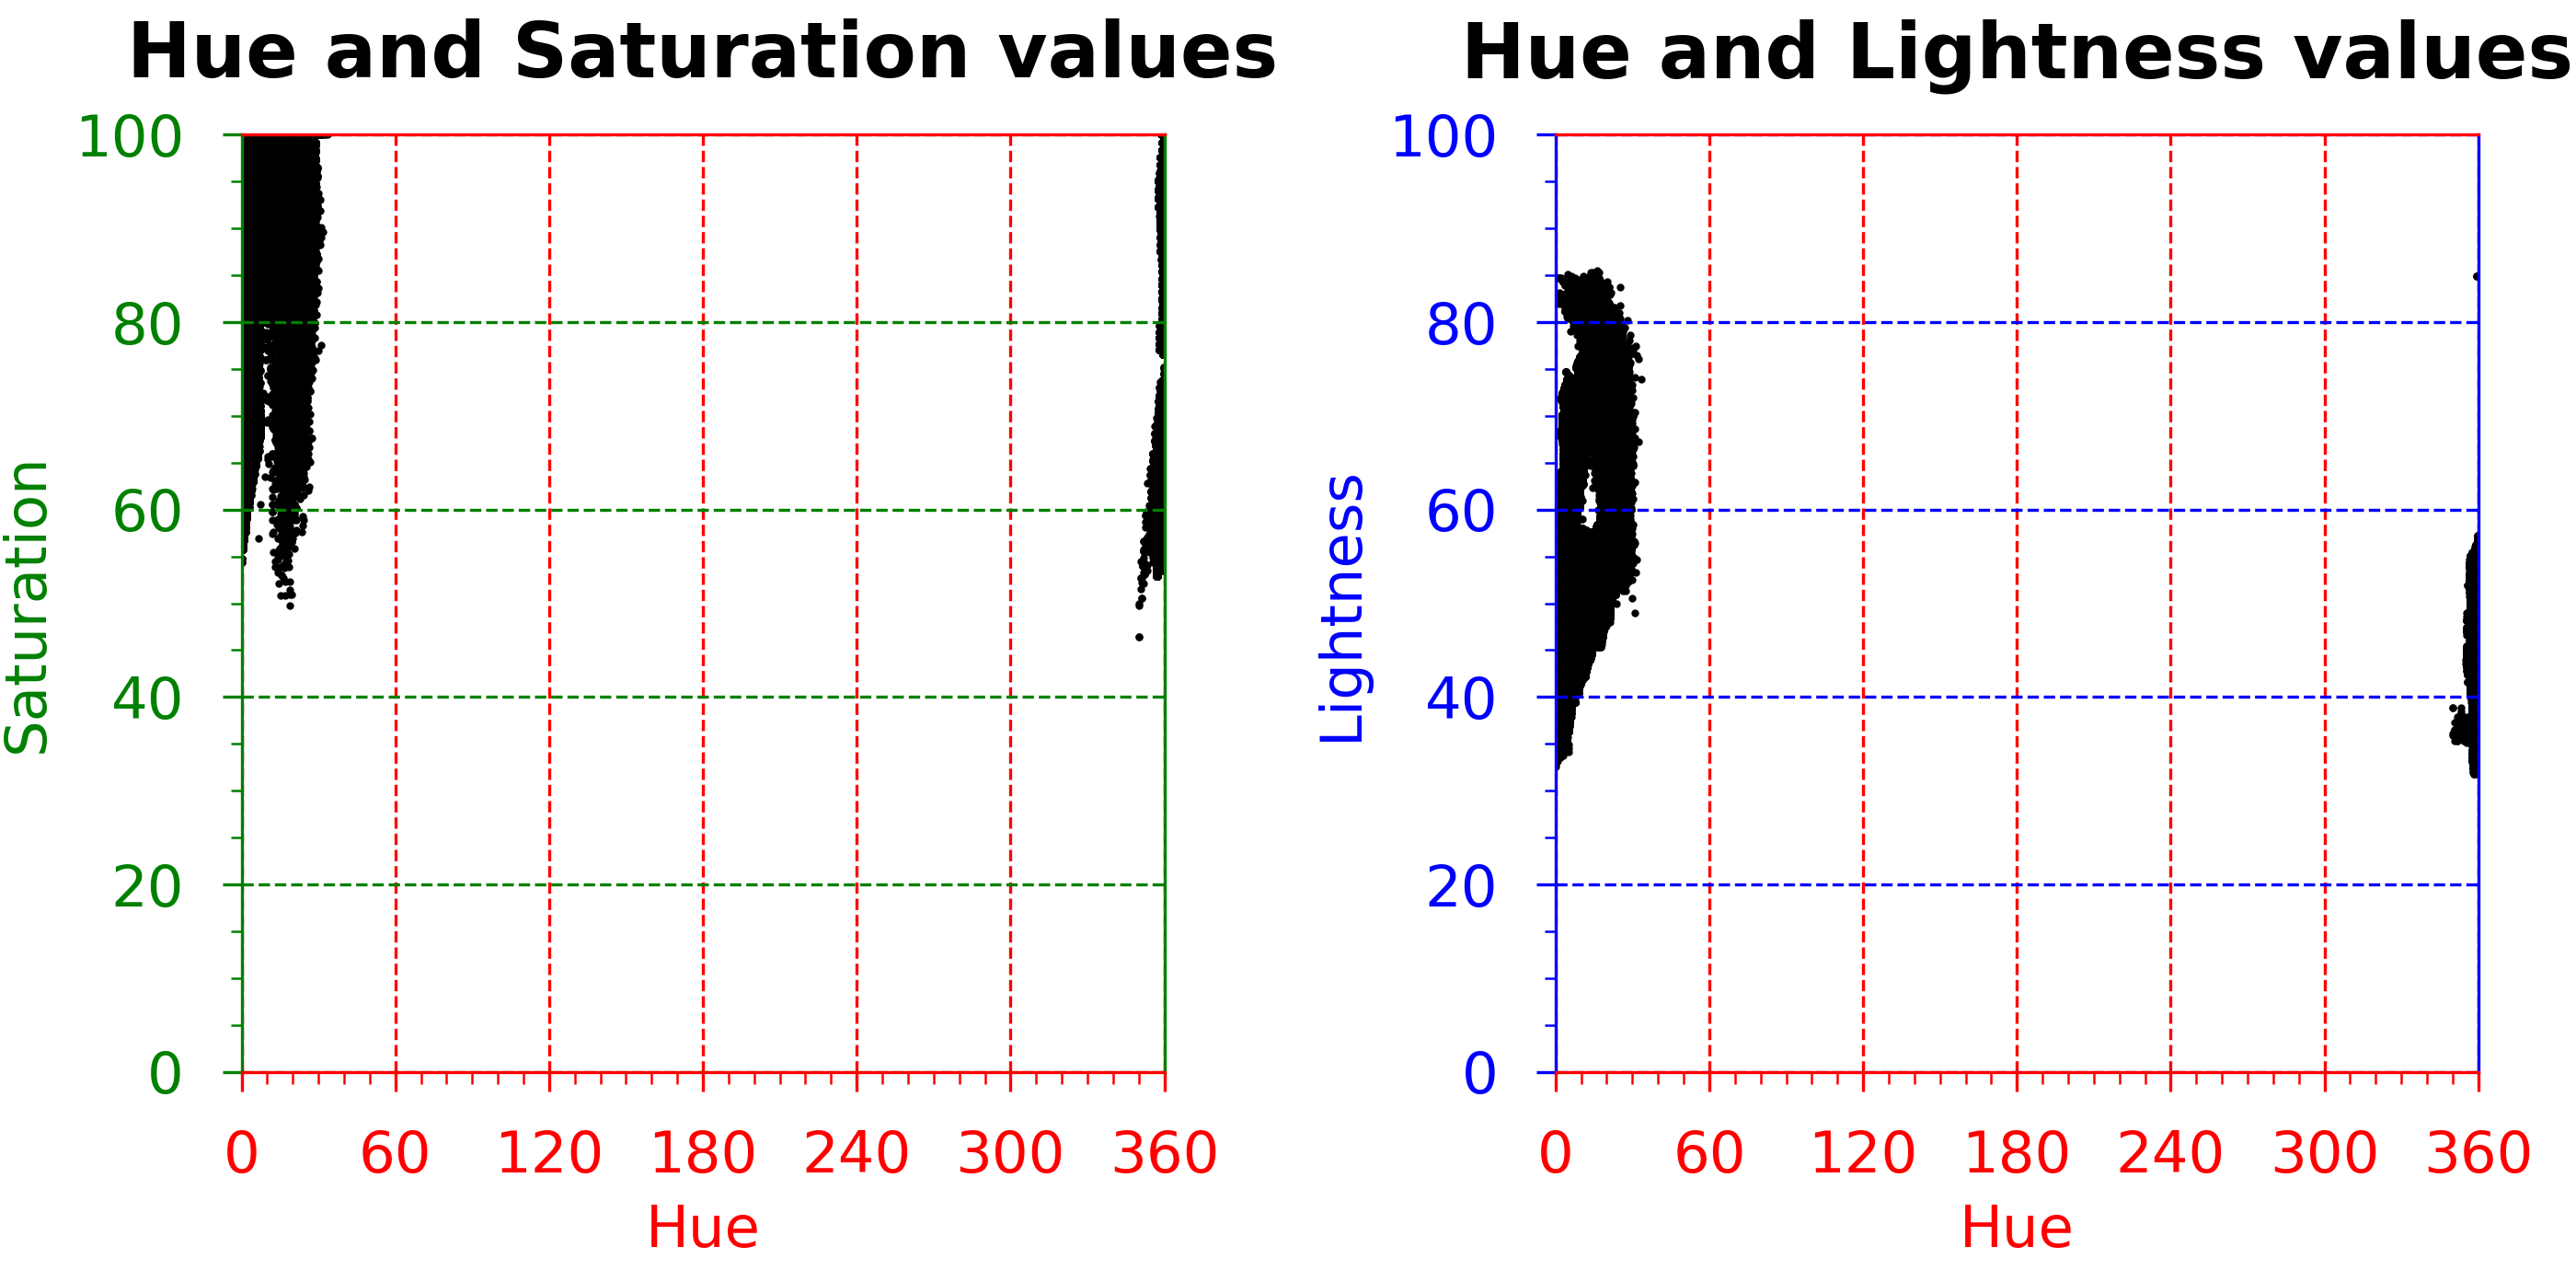
\includegraphics[width=\textwidth]{img/hslRed.png}
	\caption{Scatter plots in functie van tint en saturatie, alsook in functie van tint en lichtheid voor de kleur rood.}
	\label{hslRedPlot}
\end{figure}

\vspace{25mm}

\begin{figure}[h!]
	\center
	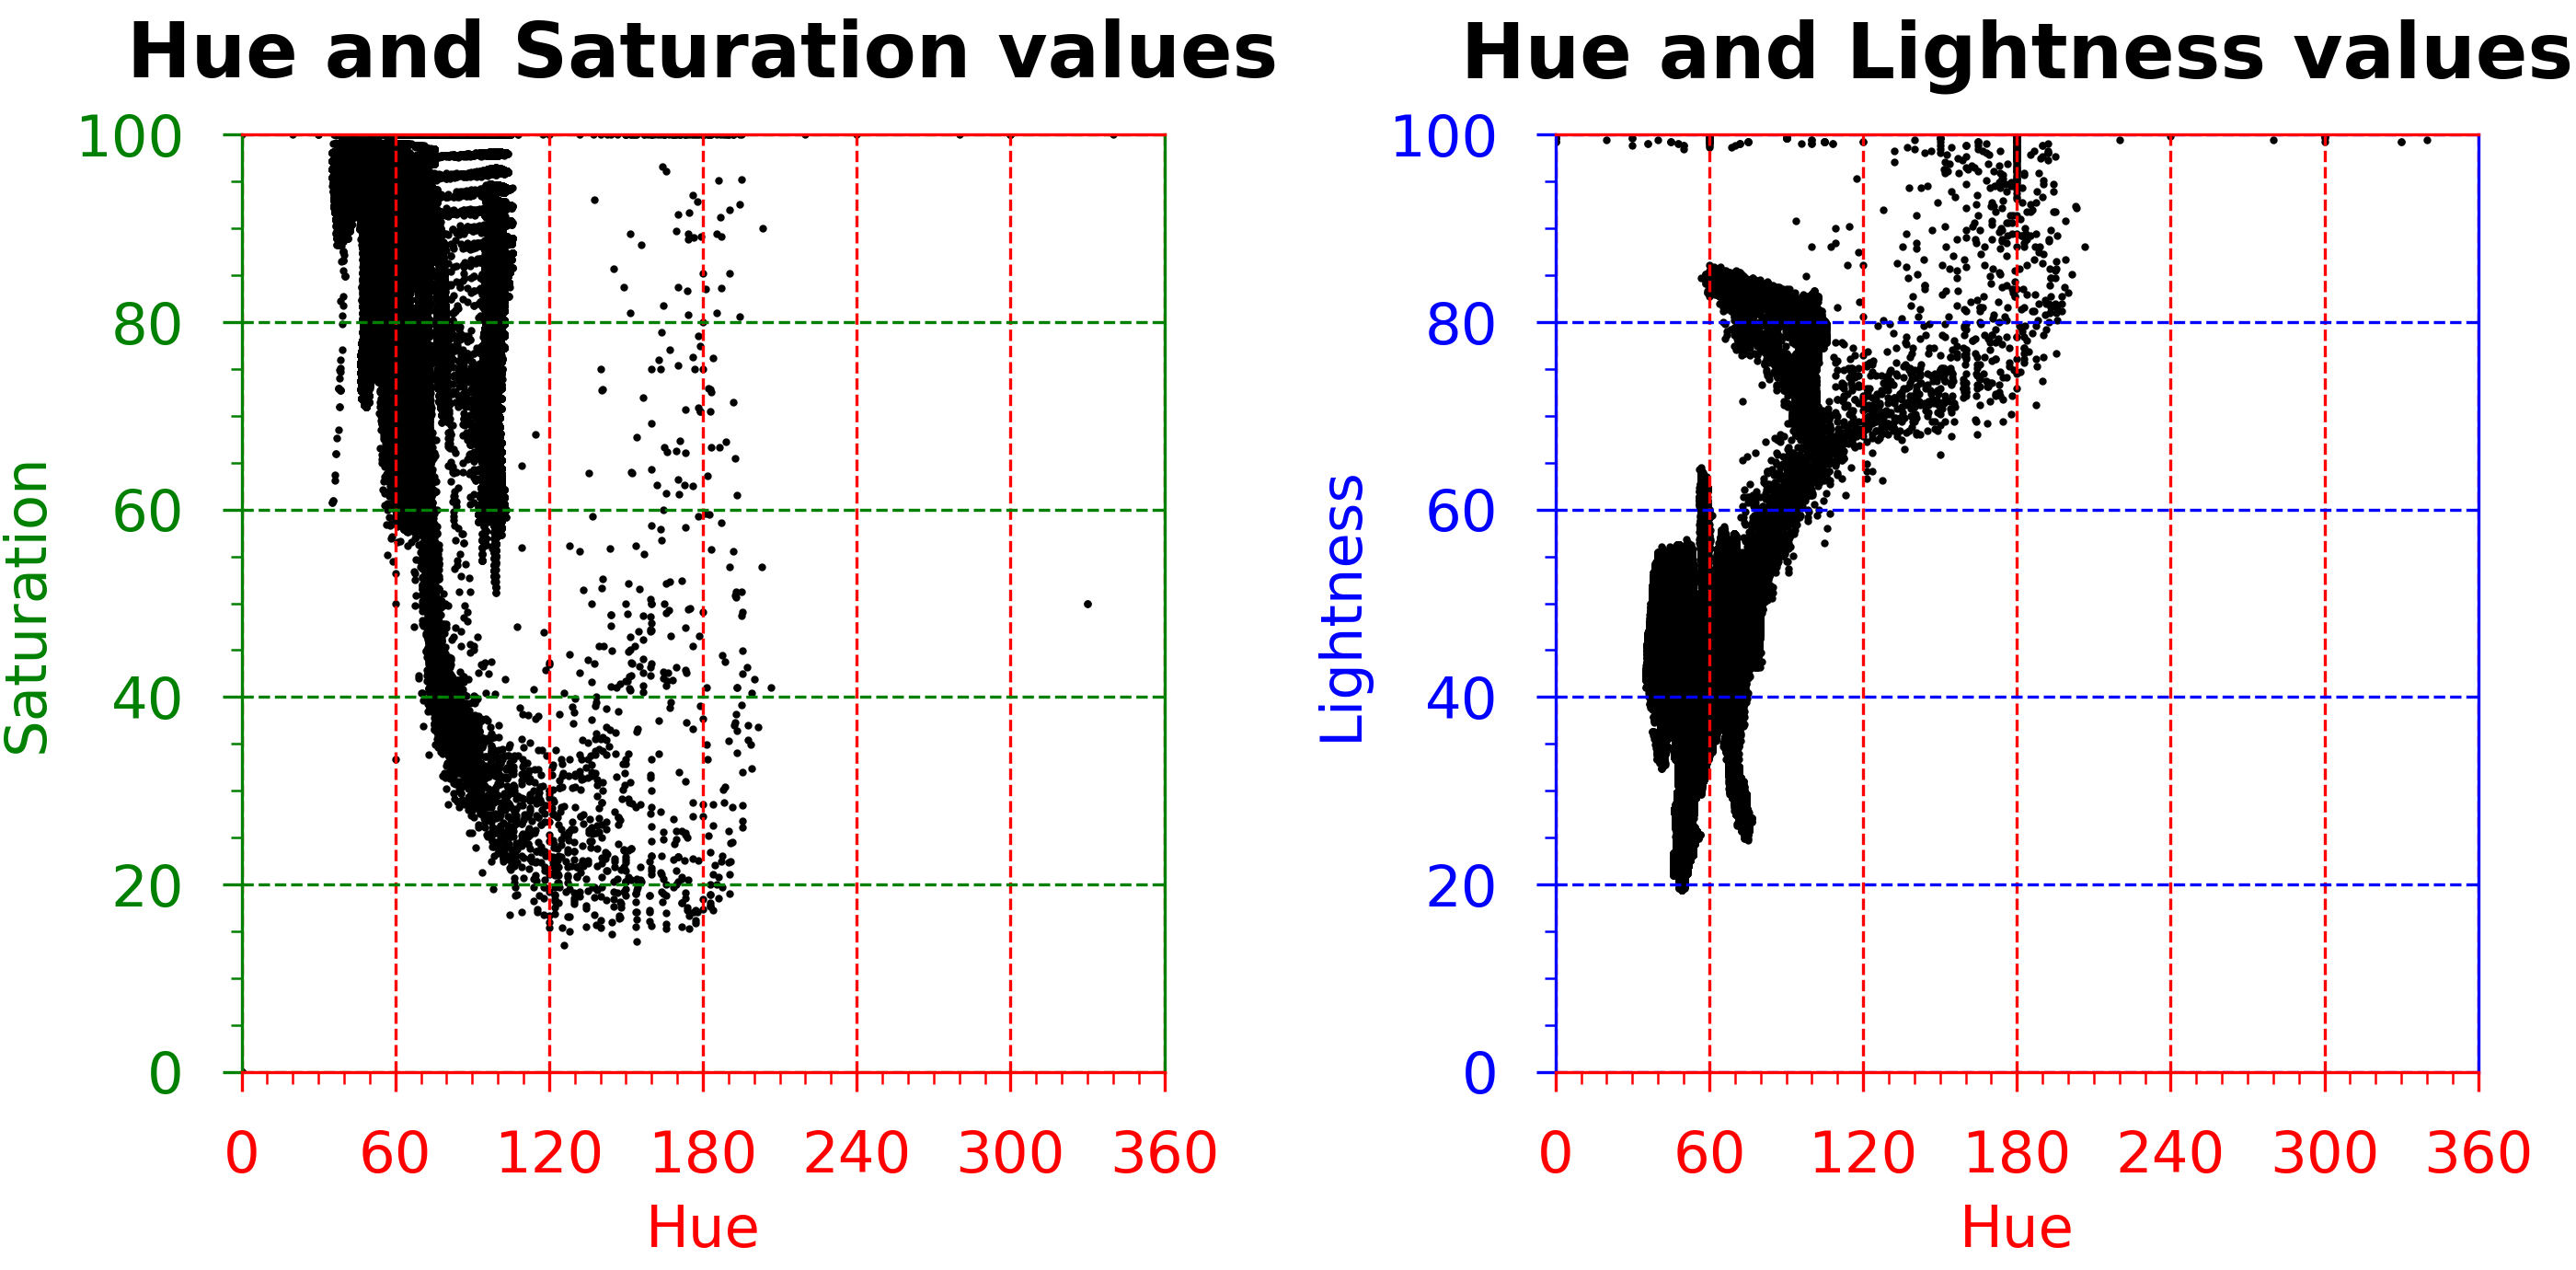
\includegraphics[width=\textwidth]{img/hslYellow.png}
	\caption{Scatter plots in functie van tint en saturatie, alsook in functie van tint en lichtheid voor de kleur geel.}
	\label{hslYellowPlot}
\end{figure}

\begin{figure}[h!]
	\center
	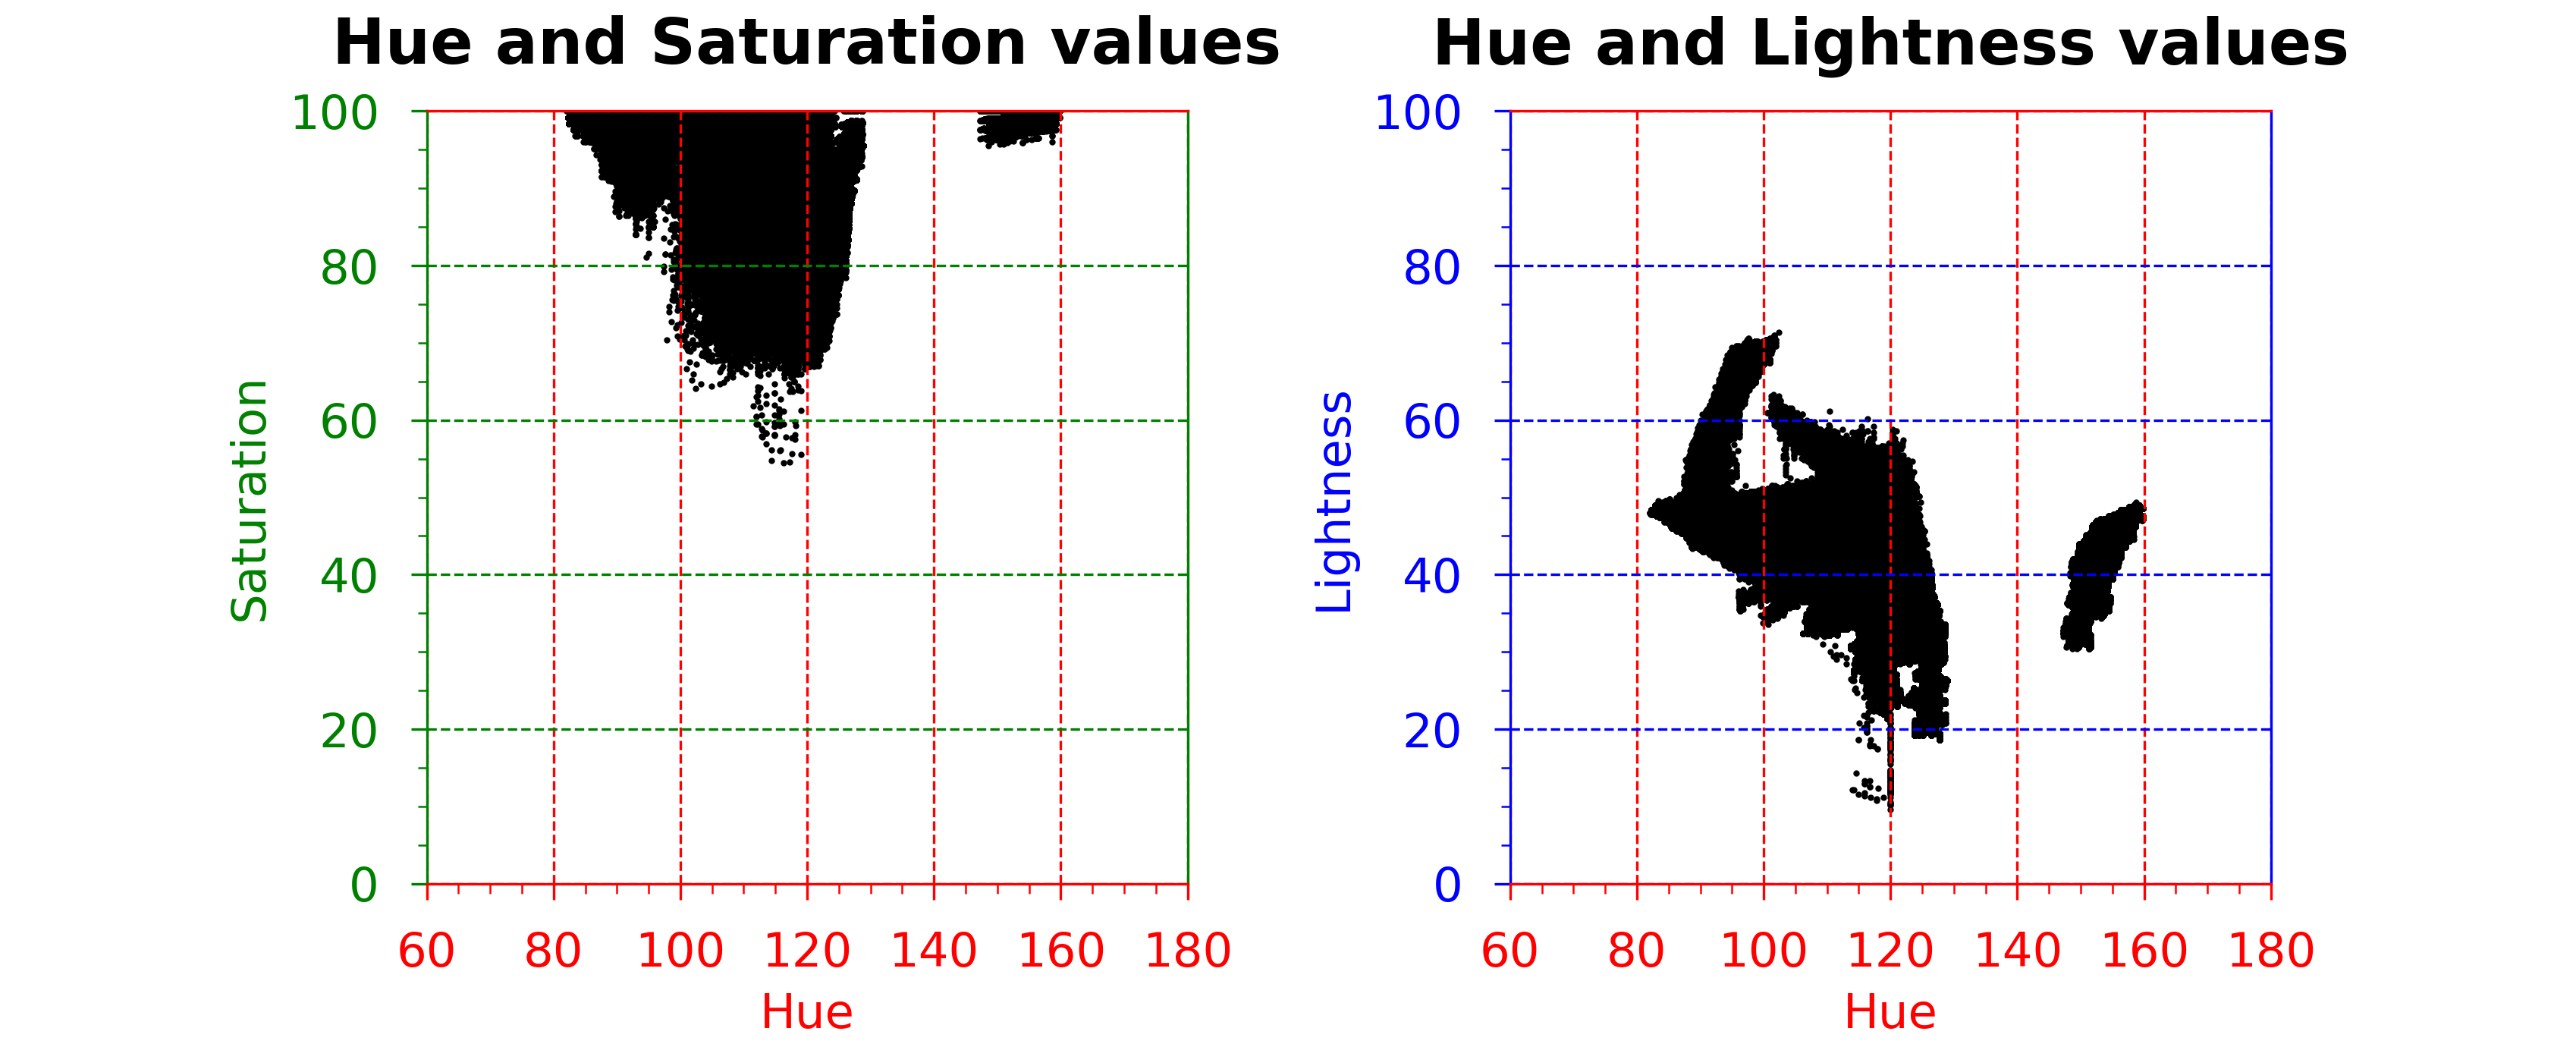
\includegraphics[width=\textwidth]{img/hslGreen.png}
	\caption{Scatter plots in functie van tint en saturatie, alsook in functie van tint en lichtheid voor de kleur groen.}
	\label{hslGreenPlot}
\end{figure}

\begin{figure}[h!]
	\center
	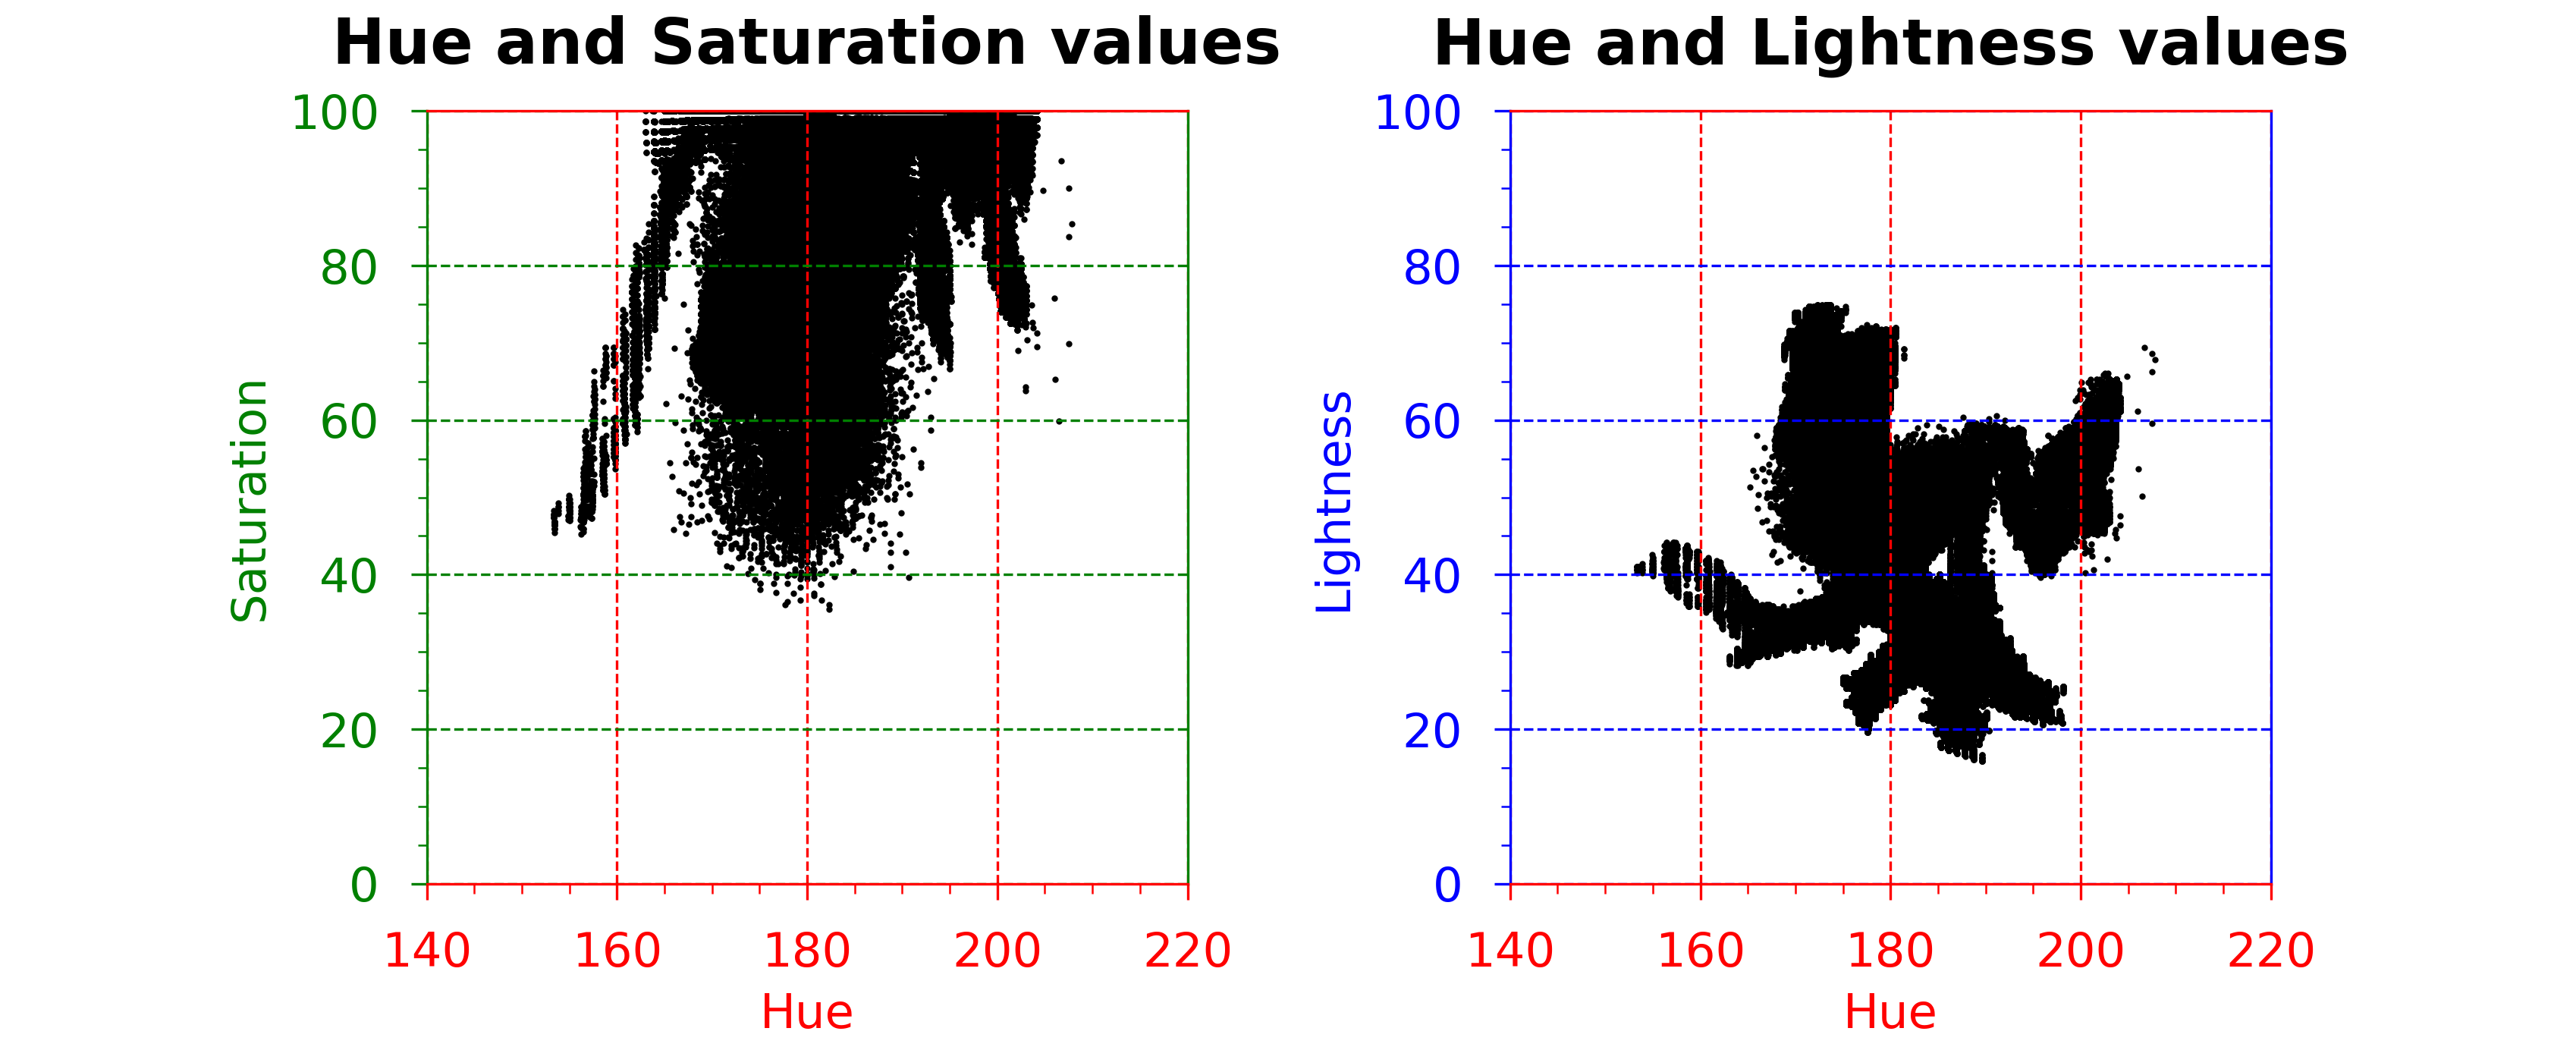
\includegraphics[width=\textwidth]{img/hslBlueGreen.png}
	\caption{Scatter plots in functie van tint en saturatie, alsook in functie van tint en lichtheid voor de kleur cyaan.}
	\label{hslBlueGreenPlot}
\end{figure}

\begin{figure}[h!]
	\center
	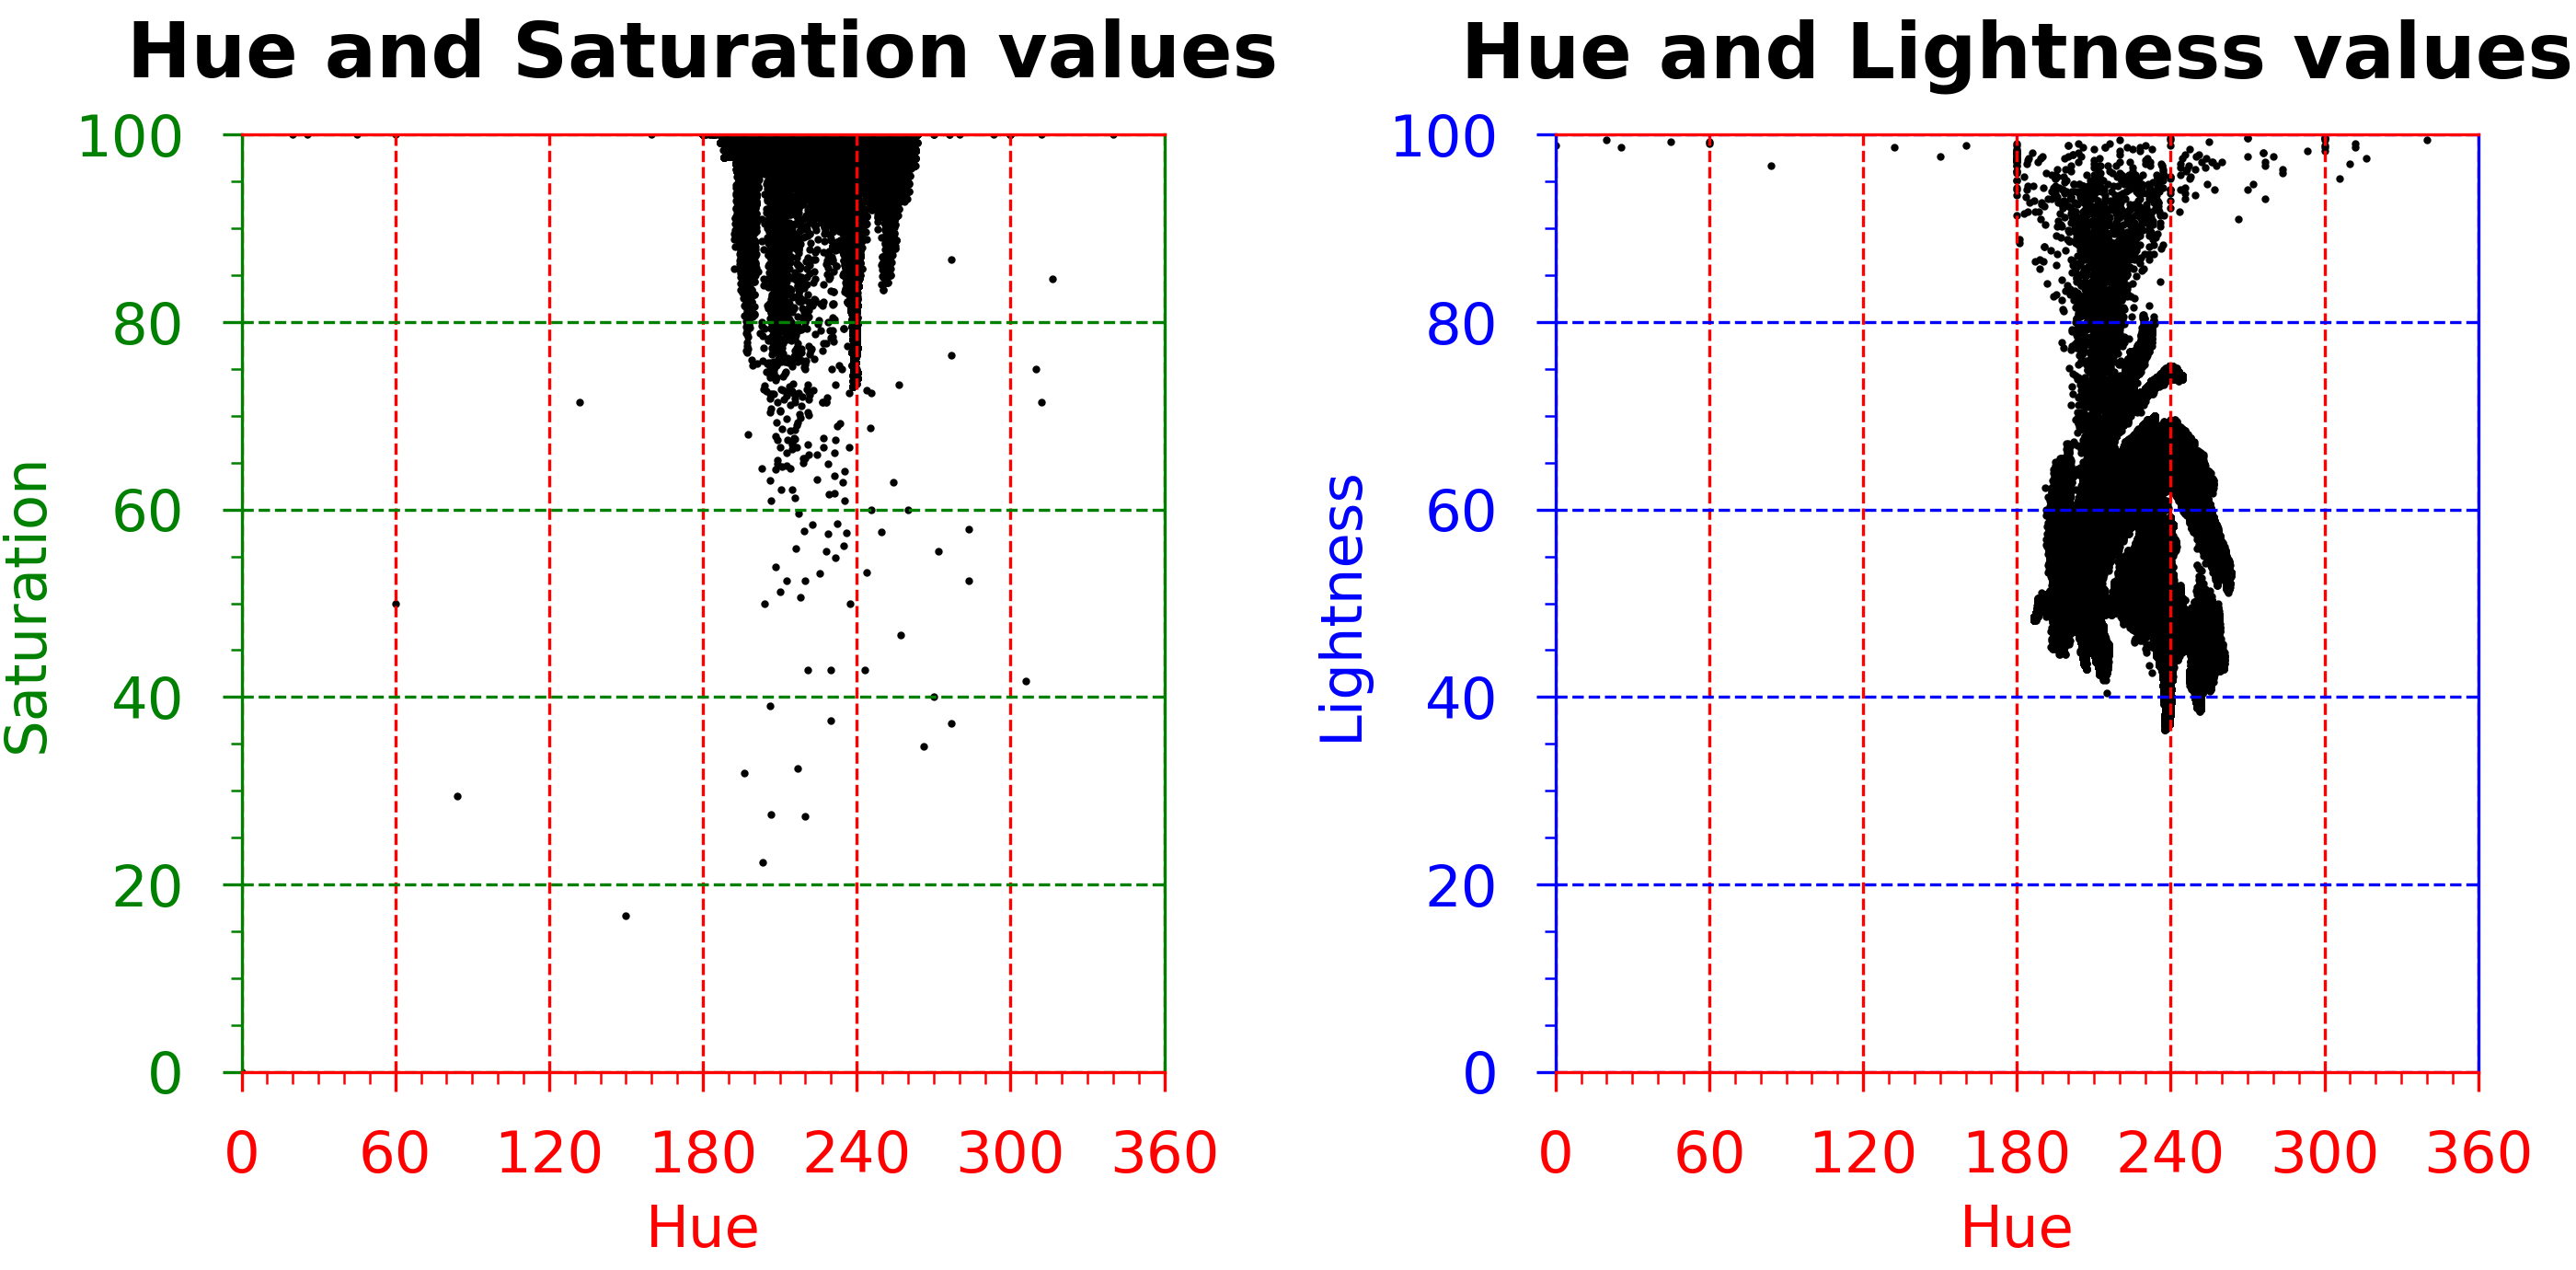
\includegraphics[width=\textwidth]{img/hslBlue.png}
	\caption{Scatter plots in functie van tint en saturatie, alsook in functie van tint en lichtheid voor de kleur blauw.}
	\label{hslBluePlot}
\end{figure}

\begin{figure}[h!]
	\center
	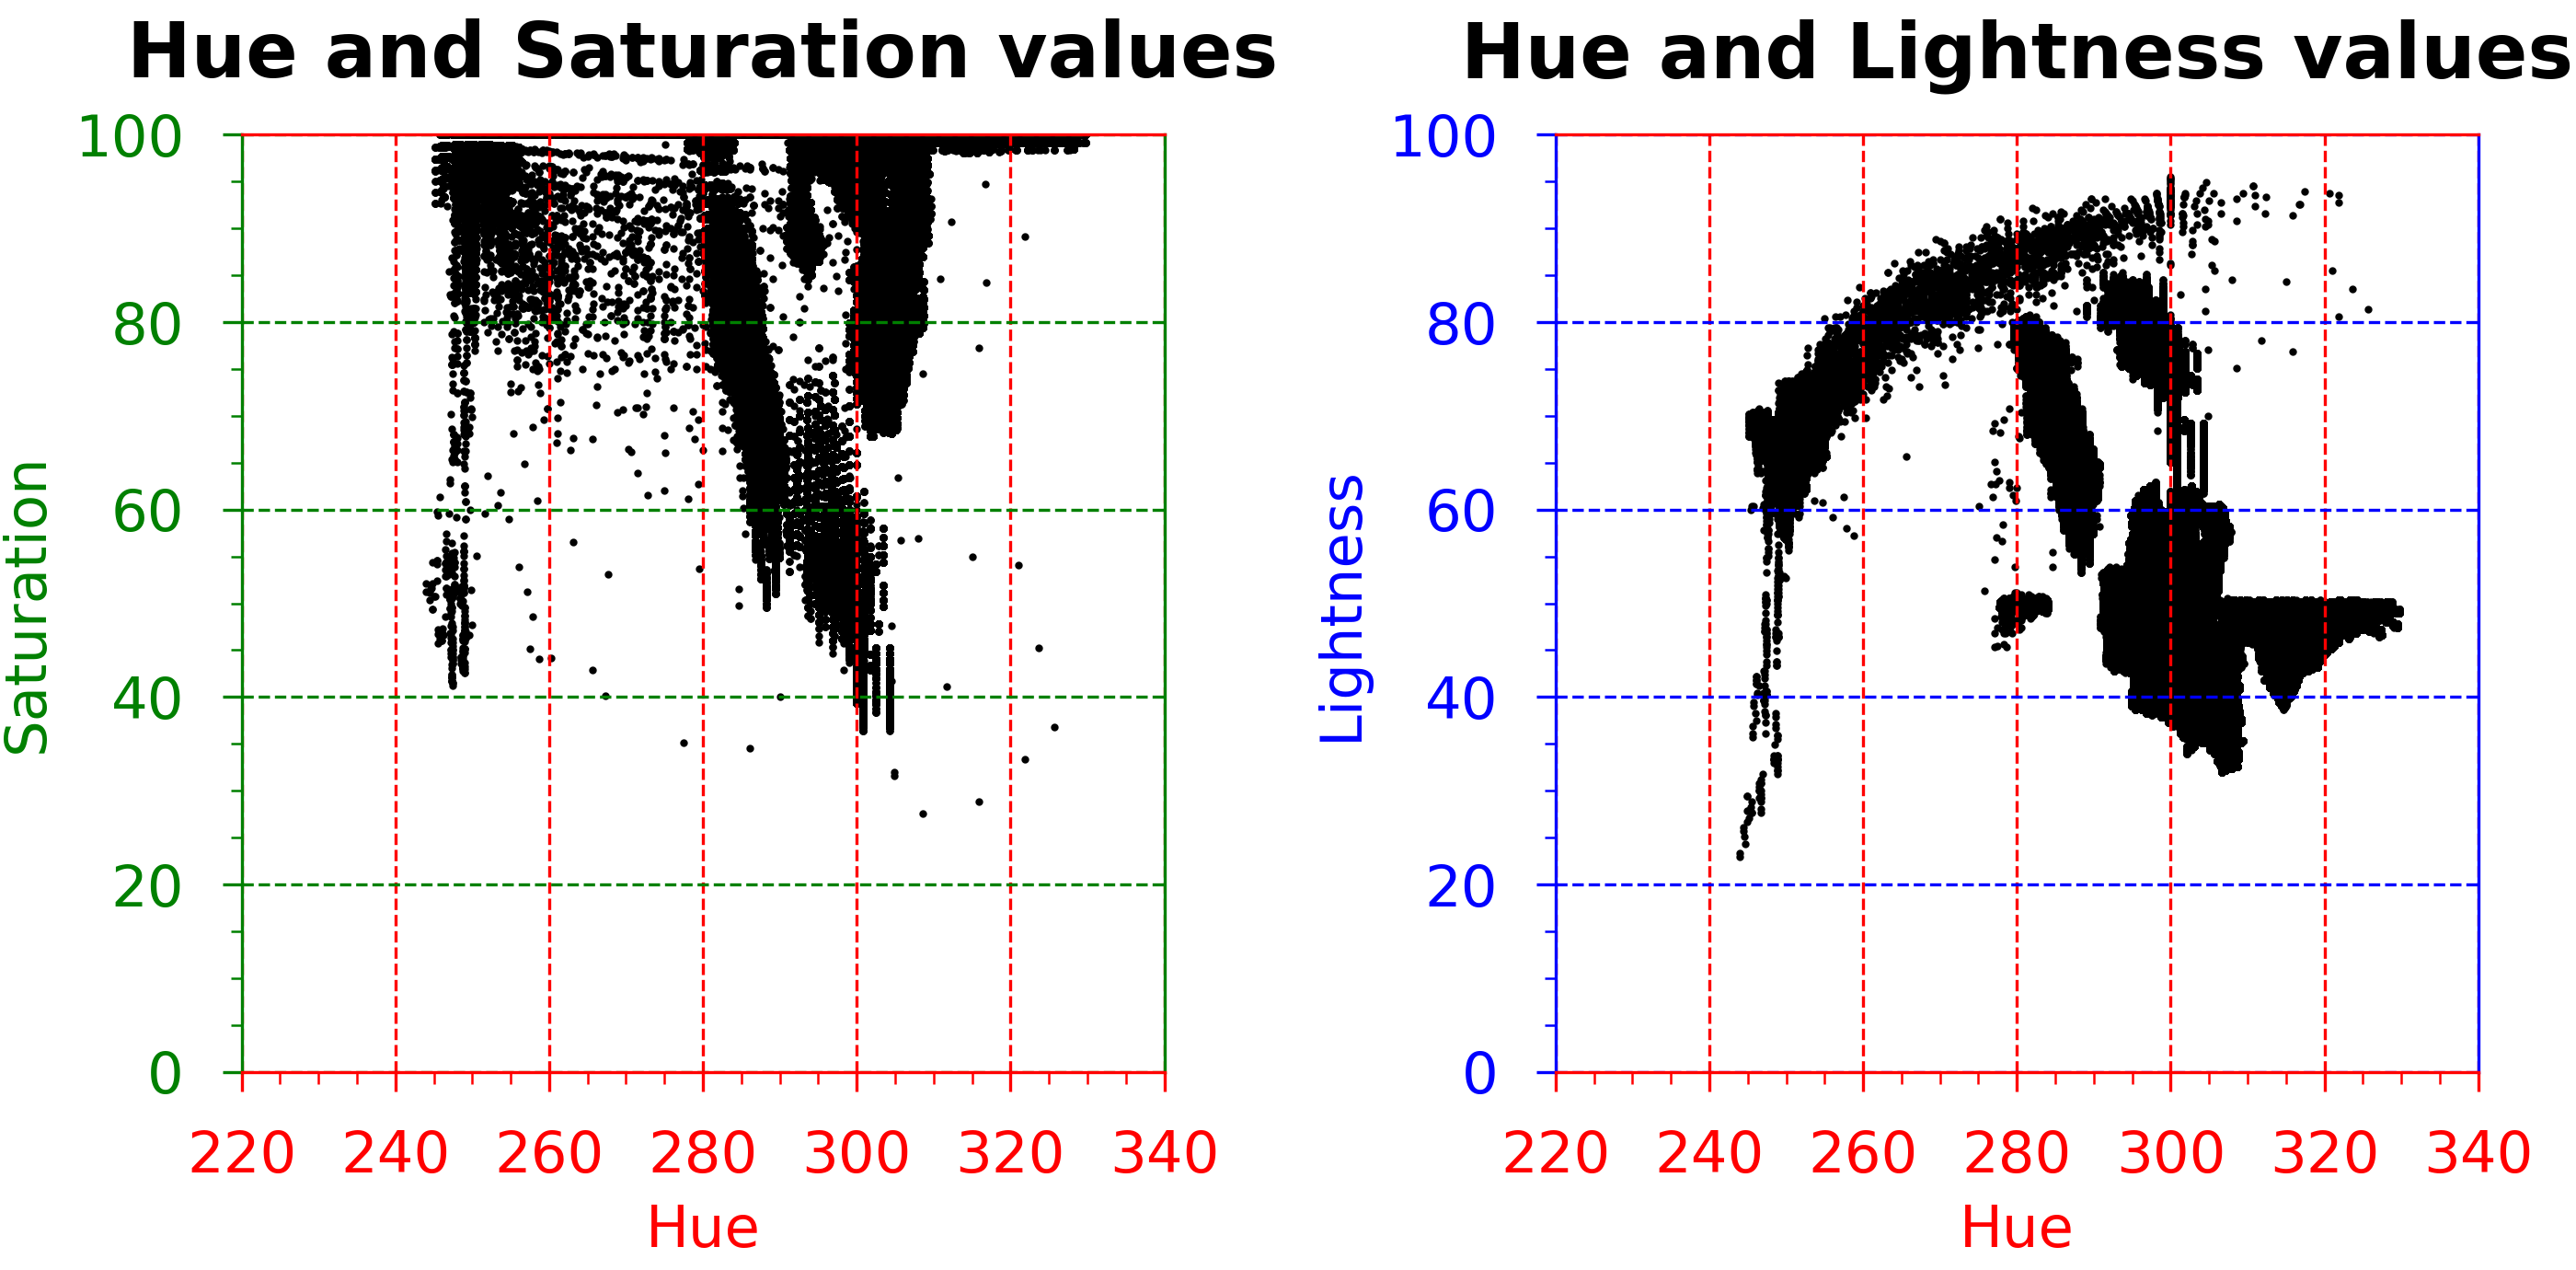
\includegraphics[width=\textwidth]{img/hslPink.png}
	\caption{Scatter plots in functie van tint en saturatie, alsook in functie van tint en lichtheid voor de kleur magenta.}
	\label{hslPinkPlot}
\end{figure}


\end{document}